\documentclass[twoside]{book}

% Packages required by doxygen
\usepackage{fixltx2e}
\usepackage{calc}
\usepackage{doxygen}
\usepackage[export]{adjustbox} % also loads graphicx
\usepackage{graphicx}
\usepackage[utf8]{inputenc}
\usepackage{makeidx}
\usepackage{multicol}
\usepackage{multirow}
\PassOptionsToPackage{warn}{textcomp}
\usepackage{textcomp}
\usepackage[nointegrals]{wasysym}
\usepackage[table]{xcolor}

% NLS support packages
\usepackage[T2A]{fontenc}
\usepackage[russian]{babel}

% Font selection
\usepackage[T1]{fontenc}
\usepackage[scaled=.90]{helvet}
\usepackage{courier}
\usepackage{amssymb}
\usepackage{sectsty}
\renewcommand{\familydefault}{\sfdefault}
\allsectionsfont{%
  \fontseries{bc}\selectfont%
  \color{darkgray}%
}
\renewcommand{\DoxyLabelFont}{%
  \fontseries{bc}\selectfont%
  \color{darkgray}%
}
\newcommand{\+}{\discretionary{\mbox{\scriptsize$\hookleftarrow$}}{}{}}

% Page & text layout
\usepackage{geometry}
\geometry{%
  a4paper,%
  top=2.5cm,%
  bottom=2.5cm,%
  left=2.5cm,%
  right=2.5cm%
}
\tolerance=750
\hfuzz=15pt
\hbadness=750
\setlength{\emergencystretch}{15pt}
\setlength{\parindent}{0cm}
\setlength{\parskip}{3ex plus 2ex minus 2ex}
\makeatletter
\renewcommand{\paragraph}{%
  \@startsection{paragraph}{4}{0ex}{-1.0ex}{1.0ex}{%
    \normalfont\normalsize\bfseries\SS@parafont%
  }%
}
\renewcommand{\subparagraph}{%
  \@startsection{subparagraph}{5}{0ex}{-1.0ex}{1.0ex}{%
    \normalfont\normalsize\bfseries\SS@subparafont%
  }%
}
\makeatother

% Headers & footers
\usepackage{fancyhdr}
\pagestyle{fancyplain}
\fancyhead[LE]{\fancyplain{}{\bfseries\thepage}}
\fancyhead[CE]{\fancyplain{}{}}
\fancyhead[RE]{\fancyplain{}{\bfseries\leftmark}}
\fancyhead[LO]{\fancyplain{}{\bfseries\rightmark}}
\fancyhead[CO]{\fancyplain{}{}}
\fancyhead[RO]{\fancyplain{}{\bfseries\thepage}}
\fancyfoot[LE]{\fancyplain{}{}}
\fancyfoot[CE]{\fancyplain{}{}}
\fancyfoot[RE]{\fancyplain{}{\bfseries\scriptsize Создано системой Doxygen }}
\fancyfoot[LO]{\fancyplain{}{\bfseries\scriptsize Создано системой Doxygen }}
\fancyfoot[CO]{\fancyplain{}{}}
\fancyfoot[RO]{\fancyplain{}{}}
\renewcommand{\footrulewidth}{0.4pt}
\renewcommand{\chaptermark}[1]{%
  \markboth{#1}{}%
}
\renewcommand{\sectionmark}[1]{%
  \markright{\thesection\ #1}%
}

% Indices & bibliography
\usepackage{natbib}
\usepackage[titles]{tocloft}
\setcounter{tocdepth}{3}
\setcounter{secnumdepth}{5}
\makeindex

% Hyperlinks (required, but should be loaded last)
\usepackage{ifpdf}
\ifpdf
  \usepackage[pdftex,pagebackref=true]{hyperref}
\else
  \usepackage[ps2pdf,pagebackref=true]{hyperref}
\fi
\hypersetup{%
  colorlinks=true,%
  linkcolor=blue,%
  citecolor=blue,%
  unicode%
}

% Custom commands
\newcommand{\clearemptydoublepage}{%
  \newpage{\pagestyle{empty}\cleardoublepage}%
}

\usepackage{caption}
\captionsetup{labelsep=space,justification=centering,font={bf},singlelinecheck=off,skip=4pt,position=top}

%===== C O N T E N T S =====

\begin{document}

% Titlepage & ToC
\hypersetup{pageanchor=false,
             bookmarksnumbered=true,
             pdfencoding=unicode
            }
\pagenumbering{alph}
\begin{titlepage}
\vspace*{7cm}
\begin{center}%
{\Large A\+S\+C\+I\+I\+Wars }\\
\vspace*{1cm}
{\large Создано системой Doxygen 1.8.12}\\
\end{center}
\end{titlepage}
\clearemptydoublepage
\pagenumbering{roman}
\tableofcontents
\clearemptydoublepage
\pagenumbering{arabic}
\hypersetup{pageanchor=true}

%--- Begin generated contents ---
\chapter{Алфавитный указатель пространств имен}
\section{Пространства имен}
Полный список пространств имен.\begin{DoxyCompactList}
\item\contentsline{section}{\hyperlink{namespace_a_s_c_i_i_wars}{A\+S\+C\+I\+I\+Wars} }{\pageref{namespace_a_s_c_i_i_wars}}{}
\item\contentsline{section}{\hyperlink{namespace_a_s_c_i_i_wars_1_1_console_graphics}{A\+S\+C\+I\+I\+Wars.\+Console\+Graphics} }{\pageref{namespace_a_s_c_i_i_wars_1_1_console_graphics}}{}
\item\contentsline{section}{\hyperlink{namespace_a_s_c_i_i_wars_1_1_game}{A\+S\+C\+I\+I\+Wars.\+Game} }{\pageref{namespace_a_s_c_i_i_wars_1_1_game}}{}
\item\contentsline{section}{\hyperlink{namespace_a_s_c_i_i_wars_1_1_util}{A\+S\+C\+I\+I\+Wars.\+Util} }{\pageref{namespace_a_s_c_i_i_wars_1_1_util}}{}
\end{DoxyCompactList}

\chapter{Иерархический список классов}
\section{Иерархия классов}
Иерархия классов.\begin{DoxyCompactList}
\item \contentsline{section}{A\+S\+C\+I\+I\+Wars.\+Application}{\pageref{class_a_s_c_i_i_wars_1_1_application}}{}
\item \contentsline{section}{A\+S\+C\+I\+I\+Wars.\+Game.\+Asset}{\pageref{class_a_s_c_i_i_wars_1_1_game_1_1_asset}}{}
\item \contentsline{section}{A\+S\+C\+I\+I\+Wars.\+Game.\+Asset\+Container}{\pageref{class_a_s_c_i_i_wars_1_1_game_1_1_asset_container}}{}
\item \contentsline{section}{A\+S\+C\+I\+I\+Wars.\+Game.\+Asset\+Group}{\pageref{class_a_s_c_i_i_wars_1_1_game_1_1_asset_group}}{}
\item \contentsline{section}{A\+S\+C\+I\+I\+Wars.\+Game.\+Branch}{\pageref{class_a_s_c_i_i_wars_1_1_game_1_1_branch}}{}
\item \contentsline{section}{A\+S\+C\+I\+I\+Wars.\+Util.\+Collections}{\pageref{class_a_s_c_i_i_wars_1_1_util_1_1_collections}}{}
\item \contentsline{section}{A\+S\+C\+I\+I\+Wars.\+Game.\+Craft}{\pageref{class_a_s_c_i_i_wars_1_1_game_1_1_craft}}{}
\item \contentsline{section}{A\+S\+C\+I\+I\+Wars.\+Game.\+Crafting\+Place}{\pageref{class_a_s_c_i_i_wars_1_1_game_1_1_crafting_place}}{}
\item \contentsline{section}{A\+S\+C\+I\+I\+Wars.\+Util.\+Dictionaries}{\pageref{class_a_s_c_i_i_wars_1_1_util_1_1_dictionaries}}{}
\item \contentsline{section}{A\+S\+C\+I\+I\+Wars.\+Game.\+Enemy}{\pageref{class_a_s_c_i_i_wars_1_1_game_1_1_enemy}}{}
\item Exception\begin{DoxyCompactList}
\item \contentsline{section}{A\+S\+C\+I\+I\+Wars.\+Game.\+Full\+Inventory\+Exception}{\pageref{class_a_s_c_i_i_wars_1_1_game_1_1_full_inventory_exception}}{}
\item \contentsline{section}{A\+S\+C\+I\+I\+Wars.\+Game.\+Game\+Over\+Exception}{\pageref{class_a_s_c_i_i_wars_1_1_game_1_1_game_over_exception}}{}
\end{DoxyCompactList}
\item \contentsline{section}{A\+S\+C\+I\+I\+Wars.\+Console\+Graphics.\+Funny\+Tasks\+Loader}{\pageref{class_a_s_c_i_i_wars_1_1_console_graphics_1_1_funny_tasks_loader}}{}
\item \contentsline{section}{A\+S\+C\+I\+I\+Wars.\+Game.\+Game\+Controller}{\pageref{class_a_s_c_i_i_wars_1_1_game_1_1_game_controller}}{}
\item \contentsline{section}{A\+S\+C\+I\+I\+Wars.\+Global\+Random}{\pageref{class_a_s_c_i_i_wars_1_1_global_random}}{}
\item \contentsline{section}{A\+S\+C\+I\+I\+Wars.\+Game.\+Inventory\+Controller}{\pageref{class_a_s_c_i_i_wars_1_1_game_1_1_inventory_controller}}{}
\item \contentsline{section}{A\+S\+C\+I\+I\+Wars.\+Game.\+Item}{\pageref{class_a_s_c_i_i_wars_1_1_game_1_1_item}}{}
\begin{DoxyCompactList}
\item \contentsline{section}{A\+S\+C\+I\+I\+Wars.\+Game.\+Consumable}{\pageref{class_a_s_c_i_i_wars_1_1_game_1_1_consumable}}{}
\begin{DoxyCompactList}
\item \contentsline{section}{A\+S\+C\+I\+I\+Wars.\+Game.\+Health\+Booster}{\pageref{class_a_s_c_i_i_wars_1_1_game_1_1_health_booster}}{}
\item \contentsline{section}{A\+S\+C\+I\+I\+Wars.\+Game.\+Health\+Potion}{\pageref{class_a_s_c_i_i_wars_1_1_game_1_1_health_potion}}{}
\end{DoxyCompactList}
\item \contentsline{section}{A\+S\+C\+I\+I\+Wars.\+Game.\+Material}{\pageref{class_a_s_c_i_i_wars_1_1_game_1_1_material}}{}
\item \contentsline{section}{A\+S\+C\+I\+I\+Wars.\+Game.\+Selectable}{\pageref{class_a_s_c_i_i_wars_1_1_game_1_1_selectable}}{}
\begin{DoxyCompactList}
\item \contentsline{section}{A\+S\+C\+I\+I\+Wars.\+Game.\+Armor}{\pageref{class_a_s_c_i_i_wars_1_1_game_1_1_armor}}{}
\item \contentsline{section}{A\+S\+C\+I\+I\+Wars.\+Game.\+Weapon}{\pageref{class_a_s_c_i_i_wars_1_1_game_1_1_weapon}}{}
\end{DoxyCompactList}
\end{DoxyCompactList}
\item \contentsline{section}{A\+S\+C\+I\+I\+Wars.\+Game.\+Item\+Container}{\pageref{class_a_s_c_i_i_wars_1_1_game_1_1_item_container}}{}
\item \contentsline{section}{A\+S\+C\+I\+I\+Wars.\+Game.\+Item\+Reference}{\pageref{class_a_s_c_i_i_wars_1_1_game_1_1_item_reference}}{}
\item \contentsline{section}{A\+S\+C\+I\+I\+Wars.\+Game.\+J\+S\+O\+N\+Armor}{\pageref{class_a_s_c_i_i_wars_1_1_game_1_1_j_s_o_n_armor}}{}
\item \contentsline{section}{A\+S\+C\+I\+I\+Wars.\+Game.\+J\+S\+O\+N\+Health\+Booster}{\pageref{class_a_s_c_i_i_wars_1_1_game_1_1_j_s_o_n_health_booster}}{}
\item \contentsline{section}{A\+S\+C\+I\+I\+Wars.\+Game.\+J\+S\+O\+N\+Health\+Potion}{\pageref{class_a_s_c_i_i_wars_1_1_game_1_1_j_s_o_n_health_potion}}{}
\item \contentsline{section}{A\+S\+C\+I\+I\+Wars.\+Game.\+J\+S\+O\+N\+Material}{\pageref{class_a_s_c_i_i_wars_1_1_game_1_1_j_s_o_n_material}}{}
\item \contentsline{section}{A\+S\+C\+I\+I\+Wars.\+Game.\+J\+S\+O\+N\+Weapon}{\pageref{class_a_s_c_i_i_wars_1_1_game_1_1_j_s_o_n_weapon}}{}
\item \contentsline{section}{A\+S\+C\+I\+I\+Wars.\+Util.\+Lambdas}{\pageref{class_a_s_c_i_i_wars_1_1_util_1_1_lambdas}}{}
\item \contentsline{section}{A\+S\+C\+I\+I\+Wars.\+Console\+Graphics.\+Loading\+Bar}{\pageref{class_a_s_c_i_i_wars_1_1_console_graphics_1_1_loading_bar}}{}
\item \contentsline{section}{A\+S\+C\+I\+I\+Wars.\+Console\+Graphics.\+Menu\+Drawer}{\pageref{class_a_s_c_i_i_wars_1_1_console_graphics_1_1_menu_drawer}}{}
\item \contentsline{section}{A\+S\+C\+I\+I\+Wars.\+Game.\+Merchant}{\pageref{class_a_s_c_i_i_wars_1_1_game_1_1_merchant}}{}
\item \contentsline{section}{A\+S\+C\+I\+I\+Wars.\+Game.\+Merchant\+Item}{\pageref{class_a_s_c_i_i_wars_1_1_game_1_1_merchant_item}}{}
\item \contentsline{section}{A\+S\+C\+I\+I\+Wars.\+Console\+Graphics.\+My\+Console}{\pageref{class_a_s_c_i_i_wars_1_1_console_graphics_1_1_my_console}}{}
\item \contentsline{section}{A\+S\+C\+I\+I\+Wars.\+Game.\+Next\+Situation}{\pageref{class_a_s_c_i_i_wars_1_1_game_1_1_next_situation}}{}
\item \contentsline{section}{A\+S\+C\+I\+I\+Wars.\+Game.\+Player}{\pageref{class_a_s_c_i_i_wars_1_1_game_1_1_player}}{}
\item \contentsline{section}{A\+S\+C\+I\+I\+Wars.\+Game.\+Quest}{\pageref{class_a_s_c_i_i_wars_1_1_game_1_1_quest}}{}
\item \contentsline{section}{A\+S\+C\+I\+I\+Wars.\+Game.\+Situation}{\pageref{class_a_s_c_i_i_wars_1_1_game_1_1_situation}}{}
\item \contentsline{section}{A\+S\+C\+I\+I\+Wars.\+Game.\+Situation\+Container}{\pageref{class_a_s_c_i_i_wars_1_1_game_1_1_situation_container}}{}
\item \contentsline{section}{A\+S\+C\+I\+I\+Wars.\+Game.\+Situation\+Controller}{\pageref{interface_a_s_c_i_i_wars_1_1_game_1_1_situation_controller}}{}
\begin{DoxyCompactList}
\item \contentsline{section}{A\+S\+C\+I\+I\+Wars.\+Game.\+Branch\+Situation\+Controller}{\pageref{class_a_s_c_i_i_wars_1_1_game_1_1_branch_situation_controller}}{}
\item \contentsline{section}{A\+S\+C\+I\+I\+Wars.\+Game.\+Crafting\+Place\+Situation\+Controller}{\pageref{class_a_s_c_i_i_wars_1_1_game_1_1_crafting_place_situation_controller}}{}
\item \contentsline{section}{A\+S\+C\+I\+I\+Wars.\+Game.\+Enemy\+Situation\+Controller}{\pageref{class_a_s_c_i_i_wars_1_1_game_1_1_enemy_situation_controller}}{}
\item \contentsline{section}{A\+S\+C\+I\+I\+Wars.\+Game.\+Merchant\+Situation\+Controller}{\pageref{class_a_s_c_i_i_wars_1_1_game_1_1_merchant_situation_controller}}{}
\item \contentsline{section}{A\+S\+C\+I\+I\+Wars.\+Game.\+Quest\+Situation\+Controller}{\pageref{class_a_s_c_i_i_wars_1_1_game_1_1_quest_situation_controller}}{}
\end{DoxyCompactList}
\item \contentsline{section}{A\+S\+C\+I\+I\+Wars.\+Game.\+Situation\+Controllers\+Registry}{\pageref{class_a_s_c_i_i_wars_1_1_game_1_1_situation_controllers_registry}}{}
\item \contentsline{section}{A\+S\+C\+I\+I\+Wars.\+Console\+Graphics.\+Task}{\pageref{class_a_s_c_i_i_wars_1_1_console_graphics_1_1_task}}{}
\end{DoxyCompactList}

\chapter{Алфавитный указатель классов}
\section{Классы}
Классы с их кратким описанием.\begin{DoxyCompactList}
\item\contentsline{section}{\hyperlink{class_a_s_c_i_i_wars_1_1_application}{A\+S\+C\+I\+I\+Wars.\+Application} }{\pageref{class_a_s_c_i_i_wars_1_1_application}}{}
\item\contentsline{section}{\hyperlink{class_a_s_c_i_i_wars_1_1_game_1_1_armor}{A\+S\+C\+I\+I\+Wars.\+Game.\+Armor} }{\pageref{class_a_s_c_i_i_wars_1_1_game_1_1_armor}}{}
\item\contentsline{section}{\hyperlink{class_a_s_c_i_i_wars_1_1_game_1_1_asset}{A\+S\+C\+I\+I\+Wars.\+Game.\+Asset} \\*Ассет. Хранит текст ассета }{\pageref{class_a_s_c_i_i_wars_1_1_game_1_1_asset}}{}
\item\contentsline{section}{\hyperlink{class_a_s_c_i_i_wars_1_1_game_1_1_asset_container}{A\+S\+C\+I\+I\+Wars.\+Game.\+Asset\+Container} \\*Контейнер ассетов. Хранит их по групам. В каждой группе находятся файлы ассетов }{\pageref{class_a_s_c_i_i_wars_1_1_game_1_1_asset_container}}{}
\item\contentsline{section}{\hyperlink{class_a_s_c_i_i_wars_1_1_game_1_1_asset_group}{A\+S\+C\+I\+I\+Wars.\+Game.\+Asset\+Group} \\*Хранит файлы с ассетами }{\pageref{class_a_s_c_i_i_wars_1_1_game_1_1_asset_group}}{}
\item\contentsline{section}{\hyperlink{class_a_s_c_i_i_wars_1_1_game_1_1_branch}{A\+S\+C\+I\+I\+Wars.\+Game.\+Branch} }{\pageref{class_a_s_c_i_i_wars_1_1_game_1_1_branch}}{}
\item\contentsline{section}{\hyperlink{class_a_s_c_i_i_wars_1_1_game_1_1_branch_situation_controller}{A\+S\+C\+I\+I\+Wars.\+Game.\+Branch\+Situation\+Controller} }{\pageref{class_a_s_c_i_i_wars_1_1_game_1_1_branch_situation_controller}}{}
\item\contentsline{section}{\hyperlink{class_a_s_c_i_i_wars_1_1_util_1_1_collections}{A\+S\+C\+I\+I\+Wars.\+Util.\+Collections} }{\pageref{class_a_s_c_i_i_wars_1_1_util_1_1_collections}}{}
\item\contentsline{section}{\hyperlink{class_a_s_c_i_i_wars_1_1_game_1_1_consumable}{A\+S\+C\+I\+I\+Wars.\+Game.\+Consumable} }{\pageref{class_a_s_c_i_i_wars_1_1_game_1_1_consumable}}{}
\item\contentsline{section}{\hyperlink{class_a_s_c_i_i_wars_1_1_game_1_1_craft}{A\+S\+C\+I\+I\+Wars.\+Game.\+Craft} }{\pageref{class_a_s_c_i_i_wars_1_1_game_1_1_craft}}{}
\item\contentsline{section}{\hyperlink{class_a_s_c_i_i_wars_1_1_game_1_1_crafting_place}{A\+S\+C\+I\+I\+Wars.\+Game.\+Crafting\+Place} }{\pageref{class_a_s_c_i_i_wars_1_1_game_1_1_crafting_place}}{}
\item\contentsline{section}{\hyperlink{class_a_s_c_i_i_wars_1_1_game_1_1_crafting_place_situation_controller}{A\+S\+C\+I\+I\+Wars.\+Game.\+Crafting\+Place\+Situation\+Controller} }{\pageref{class_a_s_c_i_i_wars_1_1_game_1_1_crafting_place_situation_controller}}{}
\item\contentsline{section}{\hyperlink{class_a_s_c_i_i_wars_1_1_util_1_1_dictionaries}{A\+S\+C\+I\+I\+Wars.\+Util.\+Dictionaries} }{\pageref{class_a_s_c_i_i_wars_1_1_util_1_1_dictionaries}}{}
\item\contentsline{section}{\hyperlink{class_a_s_c_i_i_wars_1_1_game_1_1_enemy}{A\+S\+C\+I\+I\+Wars.\+Game.\+Enemy} }{\pageref{class_a_s_c_i_i_wars_1_1_game_1_1_enemy}}{}
\item\contentsline{section}{\hyperlink{class_a_s_c_i_i_wars_1_1_game_1_1_enemy_situation_controller}{A\+S\+C\+I\+I\+Wars.\+Game.\+Enemy\+Situation\+Controller} }{\pageref{class_a_s_c_i_i_wars_1_1_game_1_1_enemy_situation_controller}}{}
\item\contentsline{section}{\hyperlink{class_a_s_c_i_i_wars_1_1_game_1_1_full_inventory_exception}{A\+S\+C\+I\+I\+Wars.\+Game.\+Full\+Inventory\+Exception} }{\pageref{class_a_s_c_i_i_wars_1_1_game_1_1_full_inventory_exception}}{}
\item\contentsline{section}{\hyperlink{class_a_s_c_i_i_wars_1_1_console_graphics_1_1_funny_tasks_loader}{A\+S\+C\+I\+I\+Wars.\+Console\+Graphics.\+Funny\+Tasks\+Loader} \\*Загружает задачи из файла со смешными названиями для задач. В файле содержатся только имена, а класс преобразует их задачи со случайным временем от \hyperlink{class_a_s_c_i_i_wars_1_1_console_graphics_1_1_funny_tasks_loader_a9008864a7b23b6e86b350b5c2097151c}{M\+I\+N\+\_\+\+T\+A\+S\+K\+\_\+\+D\+E\+L\+AY} до \hyperlink{class_a_s_c_i_i_wars_1_1_console_graphics_1_1_funny_tasks_loader_a0c34f365b46e3cc7e9974d5412b05f6c}{M\+A\+X\+\_\+\+T\+A\+S\+K\+\_\+\+D\+E\+L\+AY} }{\pageref{class_a_s_c_i_i_wars_1_1_console_graphics_1_1_funny_tasks_loader}}{}
\item\contentsline{section}{\hyperlink{class_a_s_c_i_i_wars_1_1_game_1_1_game_controller}{A\+S\+C\+I\+I\+Wars.\+Game.\+Game\+Controller} }{\pageref{class_a_s_c_i_i_wars_1_1_game_1_1_game_controller}}{}
\item\contentsline{section}{\hyperlink{class_a_s_c_i_i_wars_1_1_game_1_1_game_over_exception}{A\+S\+C\+I\+I\+Wars.\+Game.\+Game\+Over\+Exception} \\*Исключение, которое выбрасывается при окончании игры }{\pageref{class_a_s_c_i_i_wars_1_1_game_1_1_game_over_exception}}{}
\item\contentsline{section}{\hyperlink{class_a_s_c_i_i_wars_1_1_global_random}{A\+S\+C\+I\+I\+Wars.\+Global\+Random} \\*Глобальный контейнер для генератора рандамных чисел }{\pageref{class_a_s_c_i_i_wars_1_1_global_random}}{}
\item\contentsline{section}{\hyperlink{class_a_s_c_i_i_wars_1_1_game_1_1_health_booster}{A\+S\+C\+I\+I\+Wars.\+Game.\+Health\+Booster} }{\pageref{class_a_s_c_i_i_wars_1_1_game_1_1_health_booster}}{}
\item\contentsline{section}{\hyperlink{class_a_s_c_i_i_wars_1_1_game_1_1_health_potion}{A\+S\+C\+I\+I\+Wars.\+Game.\+Health\+Potion} }{\pageref{class_a_s_c_i_i_wars_1_1_game_1_1_health_potion}}{}
\item\contentsline{section}{\hyperlink{class_a_s_c_i_i_wars_1_1_game_1_1_inventory_controller}{A\+S\+C\+I\+I\+Wars.\+Game.\+Inventory\+Controller} }{\pageref{class_a_s_c_i_i_wars_1_1_game_1_1_inventory_controller}}{}
\item\contentsline{section}{\hyperlink{class_a_s_c_i_i_wars_1_1_game_1_1_item}{A\+S\+C\+I\+I\+Wars.\+Game.\+Item} }{\pageref{class_a_s_c_i_i_wars_1_1_game_1_1_item}}{}
\item\contentsline{section}{\hyperlink{class_a_s_c_i_i_wars_1_1_game_1_1_item_container}{A\+S\+C\+I\+I\+Wars.\+Game.\+Item\+Container} }{\pageref{class_a_s_c_i_i_wars_1_1_game_1_1_item_container}}{}
\item\contentsline{section}{\hyperlink{class_a_s_c_i_i_wars_1_1_game_1_1_item_reference}{A\+S\+C\+I\+I\+Wars.\+Game.\+Item\+Reference} }{\pageref{class_a_s_c_i_i_wars_1_1_game_1_1_item_reference}}{}
\item\contentsline{section}{\hyperlink{class_a_s_c_i_i_wars_1_1_game_1_1_j_s_o_n_armor}{A\+S\+C\+I\+I\+Wars.\+Game.\+J\+S\+O\+N\+Armor} }{\pageref{class_a_s_c_i_i_wars_1_1_game_1_1_j_s_o_n_armor}}{}
\item\contentsline{section}{\hyperlink{class_a_s_c_i_i_wars_1_1_game_1_1_j_s_o_n_health_booster}{A\+S\+C\+I\+I\+Wars.\+Game.\+J\+S\+O\+N\+Health\+Booster} }{\pageref{class_a_s_c_i_i_wars_1_1_game_1_1_j_s_o_n_health_booster}}{}
\item\contentsline{section}{\hyperlink{class_a_s_c_i_i_wars_1_1_game_1_1_j_s_o_n_health_potion}{A\+S\+C\+I\+I\+Wars.\+Game.\+J\+S\+O\+N\+Health\+Potion} }{\pageref{class_a_s_c_i_i_wars_1_1_game_1_1_j_s_o_n_health_potion}}{}
\item\contentsline{section}{\hyperlink{class_a_s_c_i_i_wars_1_1_game_1_1_j_s_o_n_material}{A\+S\+C\+I\+I\+Wars.\+Game.\+J\+S\+O\+N\+Material} }{\pageref{class_a_s_c_i_i_wars_1_1_game_1_1_j_s_o_n_material}}{}
\item\contentsline{section}{\hyperlink{class_a_s_c_i_i_wars_1_1_game_1_1_j_s_o_n_weapon}{A\+S\+C\+I\+I\+Wars.\+Game.\+J\+S\+O\+N\+Weapon} }{\pageref{class_a_s_c_i_i_wars_1_1_game_1_1_j_s_o_n_weapon}}{}
\item\contentsline{section}{\hyperlink{class_a_s_c_i_i_wars_1_1_util_1_1_lambdas}{A\+S\+C\+I\+I\+Wars.\+Util.\+Lambdas} }{\pageref{class_a_s_c_i_i_wars_1_1_util_1_1_lambdas}}{}
\item\contentsline{section}{\hyperlink{class_a_s_c_i_i_wars_1_1_console_graphics_1_1_loading_bar}{A\+S\+C\+I\+I\+Wars.\+Console\+Graphics.\+Loading\+Bar} \\*Рисует символьную полоску загрузки }{\pageref{class_a_s_c_i_i_wars_1_1_console_graphics_1_1_loading_bar}}{}
\item\contentsline{section}{\hyperlink{class_a_s_c_i_i_wars_1_1_game_1_1_material}{A\+S\+C\+I\+I\+Wars.\+Game.\+Material} }{\pageref{class_a_s_c_i_i_wars_1_1_game_1_1_material}}{}
\item\contentsline{section}{\hyperlink{class_a_s_c_i_i_wars_1_1_console_graphics_1_1_menu_drawer}{A\+S\+C\+I\+I\+Wars.\+Console\+Graphics.\+Menu\+Drawer} \\*Утилита для рисования меню с выбором. Выбор можно сдвигать вверх с помощью стрелки вверх, и вниз с помощью стрелки вниз. Выбор подтверждается с помощью Enter\textquotesingle{}а }{\pageref{class_a_s_c_i_i_wars_1_1_console_graphics_1_1_menu_drawer}}{}
\item\contentsline{section}{\hyperlink{class_a_s_c_i_i_wars_1_1_game_1_1_merchant}{A\+S\+C\+I\+I\+Wars.\+Game.\+Merchant} }{\pageref{class_a_s_c_i_i_wars_1_1_game_1_1_merchant}}{}
\item\contentsline{section}{\hyperlink{class_a_s_c_i_i_wars_1_1_game_1_1_merchant_item}{A\+S\+C\+I\+I\+Wars.\+Game.\+Merchant\+Item} }{\pageref{class_a_s_c_i_i_wars_1_1_game_1_1_merchant_item}}{}
\item\contentsline{section}{\hyperlink{class_a_s_c_i_i_wars_1_1_game_1_1_merchant_situation_controller}{A\+S\+C\+I\+I\+Wars.\+Game.\+Merchant\+Situation\+Controller} }{\pageref{class_a_s_c_i_i_wars_1_1_game_1_1_merchant_situation_controller}}{}
\item\contentsline{section}{\hyperlink{class_a_s_c_i_i_wars_1_1_console_graphics_1_1_my_console}{A\+S\+C\+I\+I\+Wars.\+Console\+Graphics.\+My\+Console} }{\pageref{class_a_s_c_i_i_wars_1_1_console_graphics_1_1_my_console}}{}
\item\contentsline{section}{\hyperlink{class_a_s_c_i_i_wars_1_1_game_1_1_next_situation}{A\+S\+C\+I\+I\+Wars.\+Game.\+Next\+Situation} }{\pageref{class_a_s_c_i_i_wars_1_1_game_1_1_next_situation}}{}
\item\contentsline{section}{\hyperlink{class_a_s_c_i_i_wars_1_1_game_1_1_player}{A\+S\+C\+I\+I\+Wars.\+Game.\+Player} \\*Представляет игрока }{\pageref{class_a_s_c_i_i_wars_1_1_game_1_1_player}}{}
\item\contentsline{section}{\hyperlink{class_a_s_c_i_i_wars_1_1_game_1_1_quest}{A\+S\+C\+I\+I\+Wars.\+Game.\+Quest} }{\pageref{class_a_s_c_i_i_wars_1_1_game_1_1_quest}}{}
\item\contentsline{section}{\hyperlink{class_a_s_c_i_i_wars_1_1_game_1_1_quest_situation_controller}{A\+S\+C\+I\+I\+Wars.\+Game.\+Quest\+Situation\+Controller} }{\pageref{class_a_s_c_i_i_wars_1_1_game_1_1_quest_situation_controller}}{}
\item\contentsline{section}{\hyperlink{class_a_s_c_i_i_wars_1_1_game_1_1_selectable}{A\+S\+C\+I\+I\+Wars.\+Game.\+Selectable} }{\pageref{class_a_s_c_i_i_wars_1_1_game_1_1_selectable}}{}
\item\contentsline{section}{\hyperlink{class_a_s_c_i_i_wars_1_1_game_1_1_situation}{A\+S\+C\+I\+I\+Wars.\+Game.\+Situation} }{\pageref{class_a_s_c_i_i_wars_1_1_game_1_1_situation}}{}
\item\contentsline{section}{\hyperlink{class_a_s_c_i_i_wars_1_1_game_1_1_situation_container}{A\+S\+C\+I\+I\+Wars.\+Game.\+Situation\+Container} }{\pageref{class_a_s_c_i_i_wars_1_1_game_1_1_situation_container}}{}
\item\contentsline{section}{\hyperlink{interface_a_s_c_i_i_wars_1_1_game_1_1_situation_controller}{A\+S\+C\+I\+I\+Wars.\+Game.\+Situation\+Controller} \\*Контроллер для ситуаций. Используется, если тип ситуации совпадает с ID контроллера }{\pageref{interface_a_s_c_i_i_wars_1_1_game_1_1_situation_controller}}{}
\item\contentsline{section}{\hyperlink{class_a_s_c_i_i_wars_1_1_game_1_1_situation_controllers_registry}{A\+S\+C\+I\+I\+Wars.\+Game.\+Situation\+Controllers\+Registry} \\*Содержит контроллеры ситуаций по ID\textquotesingle{}шникам }{\pageref{class_a_s_c_i_i_wars_1_1_game_1_1_situation_controllers_registry}}{}
\item\contentsline{section}{\hyperlink{class_a_s_c_i_i_wars_1_1_console_graphics_1_1_task}{A\+S\+C\+I\+I\+Wars.\+Console\+Graphics.\+Task} }{\pageref{class_a_s_c_i_i_wars_1_1_console_graphics_1_1_task}}{}
\item\contentsline{section}{\hyperlink{class_a_s_c_i_i_wars_1_1_game_1_1_weapon}{A\+S\+C\+I\+I\+Wars.\+Game.\+Weapon} }{\pageref{class_a_s_c_i_i_wars_1_1_game_1_1_weapon}}{}
\end{DoxyCompactList}

\chapter{Пространства имен}
\hypertarget{namespace_a_s_c_i_i_wars}{}\section{Пространство имен A\+S\+C\+I\+I\+Wars}
\label{namespace_a_s_c_i_i_wars}\index{A\+S\+C\+I\+I\+Wars@{A\+S\+C\+I\+I\+Wars}}
\subsection*{Пространства имен}
\begin{DoxyCompactItemize}
\item 
namespace \hyperlink{namespace_a_s_c_i_i_wars_1_1_console_graphics}{Console\+Graphics}
\item 
namespace \hyperlink{namespace_a_s_c_i_i_wars_1_1_game}{Game}
\item 
namespace \hyperlink{namespace_a_s_c_i_i_wars_1_1_util}{Util}
\end{DoxyCompactItemize}
\subsection*{Классы}
\begin{DoxyCompactItemize}
\item 
class \hyperlink{class_a_s_c_i_i_wars_1_1_application}{Application}
\item 
class \hyperlink{class_a_s_c_i_i_wars_1_1_global_random}{Global\+Random}
\begin{DoxyCompactList}\small\item\em Глобальный контейнер для генератора рандамных чисел. \end{DoxyCompactList}\end{DoxyCompactItemize}
\subsection*{Перечисления}
\begin{DoxyCompactItemize}
\item 
enum \hyperlink{namespace_a_s_c_i_i_wars_a9b8588e75dba14ac63aa79a49dd5a4eb}{Menu\+State} \{ \newline
\hyperlink{namespace_a_s_c_i_i_wars_a9b8588e75dba14ac63aa79a49dd5a4ebaad1111b48f98329333237912fc3b371b}{Menu\+State.\+Main\+Menu}, 
\hyperlink{namespace_a_s_c_i_i_wars_a9b8588e75dba14ac63aa79a49dd5a4eba31947c4eece1b08b70e9ba88dae24416}{Menu\+State.\+New\+Game}, 
\hyperlink{namespace_a_s_c_i_i_wars_a9b8588e75dba14ac63aa79a49dd5a4eba1613dbfa6c7c385e7aea951a03f93f58}{Menu\+State.\+Load\+Game}, 
\hyperlink{namespace_a_s_c_i_i_wars_a9b8588e75dba14ac63aa79a49dd5a4ebaf4f70727dc34561dfde1a3c529b6205c}{Menu\+State.\+Settings}, 
\newline
\hyperlink{namespace_a_s_c_i_i_wars_a9b8588e75dba14ac63aa79a49dd5a4eba4166c4566d4ee3c335e2f09f7f0d5d0b}{Menu\+State.\+Exit\+Game}
 \}
\end{DoxyCompactItemize}


\subsection{Перечисления}
\hypertarget{namespace_a_s_c_i_i_wars_a9b8588e75dba14ac63aa79a49dd5a4eb}{}\label{namespace_a_s_c_i_i_wars_a9b8588e75dba14ac63aa79a49dd5a4eb} 
\index{A\+S\+C\+I\+I\+Wars@{A\+S\+C\+I\+I\+Wars}!Menu\+State@{Menu\+State}}
\index{Menu\+State@{Menu\+State}!A\+S\+C\+I\+I\+Wars@{A\+S\+C\+I\+I\+Wars}}
\subsubsection{\texorpdfstring{Menu\+State}{MenuState}}
{\footnotesize\ttfamily enum \hyperlink{namespace_a_s_c_i_i_wars_a9b8588e75dba14ac63aa79a49dd5a4eb}{A\+S\+C\+I\+I\+Wars.\+Menu\+State}\hspace{0.3cm}{\ttfamily [strong]}}

\begin{DoxyEnumFields}{Элементы перечислений}
\raisebox{\heightof{T}}[0pt][0pt]{\index{Main\+Menu@{Main\+Menu}!A\+S\+C\+I\+I\+Wars@{A\+S\+C\+I\+I\+Wars}}\index{A\+S\+C\+I\+I\+Wars@{A\+S\+C\+I\+I\+Wars}!Main\+Menu@{Main\+Menu}}}\hypertarget{namespace_a_s_c_i_i_wars_a9b8588e75dba14ac63aa79a49dd5a4ebaad1111b48f98329333237912fc3b371b}{}\label{namespace_a_s_c_i_i_wars_a9b8588e75dba14ac63aa79a49dd5a4ebaad1111b48f98329333237912fc3b371b} 
Main\+Menu&\\
\hline

\raisebox{\heightof{T}}[0pt][0pt]{\index{New\+Game@{New\+Game}!A\+S\+C\+I\+I\+Wars@{A\+S\+C\+I\+I\+Wars}}\index{A\+S\+C\+I\+I\+Wars@{A\+S\+C\+I\+I\+Wars}!New\+Game@{New\+Game}}}\hypertarget{namespace_a_s_c_i_i_wars_a9b8588e75dba14ac63aa79a49dd5a4eba31947c4eece1b08b70e9ba88dae24416}{}\label{namespace_a_s_c_i_i_wars_a9b8588e75dba14ac63aa79a49dd5a4eba31947c4eece1b08b70e9ba88dae24416} 
New\+Game&\\
\hline

\raisebox{\heightof{T}}[0pt][0pt]{\index{Load\+Game@{Load\+Game}!A\+S\+C\+I\+I\+Wars@{A\+S\+C\+I\+I\+Wars}}\index{A\+S\+C\+I\+I\+Wars@{A\+S\+C\+I\+I\+Wars}!Load\+Game@{Load\+Game}}}\hypertarget{namespace_a_s_c_i_i_wars_a9b8588e75dba14ac63aa79a49dd5a4eba1613dbfa6c7c385e7aea951a03f93f58}{}\label{namespace_a_s_c_i_i_wars_a9b8588e75dba14ac63aa79a49dd5a4eba1613dbfa6c7c385e7aea951a03f93f58} 
Load\+Game&\\
\hline

\raisebox{\heightof{T}}[0pt][0pt]{\index{Settings@{Settings}!A\+S\+C\+I\+I\+Wars@{A\+S\+C\+I\+I\+Wars}}\index{A\+S\+C\+I\+I\+Wars@{A\+S\+C\+I\+I\+Wars}!Settings@{Settings}}}\hypertarget{namespace_a_s_c_i_i_wars_a9b8588e75dba14ac63aa79a49dd5a4ebaf4f70727dc34561dfde1a3c529b6205c}{}\label{namespace_a_s_c_i_i_wars_a9b8588e75dba14ac63aa79a49dd5a4ebaf4f70727dc34561dfde1a3c529b6205c} 
Settings&\\
\hline

\raisebox{\heightof{T}}[0pt][0pt]{\index{Exit\+Game@{Exit\+Game}!A\+S\+C\+I\+I\+Wars@{A\+S\+C\+I\+I\+Wars}}\index{A\+S\+C\+I\+I\+Wars@{A\+S\+C\+I\+I\+Wars}!Exit\+Game@{Exit\+Game}}}\hypertarget{namespace_a_s_c_i_i_wars_a9b8588e75dba14ac63aa79a49dd5a4eba4166c4566d4ee3c335e2f09f7f0d5d0b}{}\label{namespace_a_s_c_i_i_wars_a9b8588e75dba14ac63aa79a49dd5a4eba4166c4566d4ee3c335e2f09f7f0d5d0b} 
Exit\+Game&\\
\hline

\end{DoxyEnumFields}

\hypertarget{namespace_a_s_c_i_i_wars_1_1_console_graphics}{}\section{Пространство имен A\+S\+C\+I\+I\+Wars.\+Console\+Graphics}
\label{namespace_a_s_c_i_i_wars_1_1_console_graphics}\index{A\+S\+C\+I\+I\+Wars.\+Console\+Graphics@{A\+S\+C\+I\+I\+Wars.\+Console\+Graphics}}
\subsection*{Классы}
\begin{DoxyCompactItemize}
\item 
class \hyperlink{class_a_s_c_i_i_wars_1_1_console_graphics_1_1_funny_tasks_loader}{Funny\+Tasks\+Loader}
\begin{DoxyCompactList}\small\item\em Загружает задачи из файла со смешными названиями для задач. В файле содержатся только имена, а класс преобразует их задачи со случайным временем от \hyperlink{class_a_s_c_i_i_wars_1_1_console_graphics_1_1_funny_tasks_loader_a9008864a7b23b6e86b350b5c2097151c}{M\+I\+N\+\_\+\+T\+A\+S\+K\+\_\+\+D\+E\+L\+AY} до \hyperlink{class_a_s_c_i_i_wars_1_1_console_graphics_1_1_funny_tasks_loader_a0c34f365b46e3cc7e9974d5412b05f6c}{M\+A\+X\+\_\+\+T\+A\+S\+K\+\_\+\+D\+E\+L\+AY}. \end{DoxyCompactList}\item 
class \hyperlink{class_a_s_c_i_i_wars_1_1_console_graphics_1_1_loading_bar}{Loading\+Bar}
\begin{DoxyCompactList}\small\item\em Рисует символьную полоску загрузки. \end{DoxyCompactList}\item 
class \hyperlink{class_a_s_c_i_i_wars_1_1_console_graphics_1_1_menu_drawer}{Menu\+Drawer}
\begin{DoxyCompactList}\small\item\em Утилита для рисования меню с выбором. Выбор можно сдвигать вверх с помощью стрелки вверх, и вниз с помощью стрелки вниз. Выбор подтверждается с помощью Enter\textquotesingle{}а. \end{DoxyCompactList}\item 
class \hyperlink{class_a_s_c_i_i_wars_1_1_console_graphics_1_1_my_console}{My\+Console}
\item 
class \hyperlink{class_a_s_c_i_i_wars_1_1_console_graphics_1_1_task}{Task}
\end{DoxyCompactItemize}
\subsection*{Перечисления}
\begin{DoxyCompactItemize}
\item 
enum \hyperlink{namespace_a_s_c_i_i_wars_1_1_console_graphics_a9b323f4b2bf48062c9245b24e74b2882}{Console\+Style} \{ \hyperlink{namespace_a_s_c_i_i_wars_1_1_console_graphics_a9b323f4b2bf48062c9245b24e74b2882aaf0ab25243139e9c44bdbfbde2ce6f1d}{Console\+Style.\+No\+Style}, 
\hyperlink{namespace_a_s_c_i_i_wars_1_1_console_graphics_a9b323f4b2bf48062c9245b24e74b2882a114c3050111d8b8ddd830b99ccebd246}{Console\+Style.\+Bold}, 
\hyperlink{namespace_a_s_c_i_i_wars_1_1_console_graphics_a9b323f4b2bf48062c9245b24e74b2882a1d874710ccdcd46b95397049d2e7500c}{Console\+Style.\+Italic}, 
\hyperlink{namespace_a_s_c_i_i_wars_1_1_console_graphics_a9b323f4b2bf48062c9245b24e74b2882a852721aa5fc738dfedff2945d71da439}{Console\+Style.\+Underline}
 \}
\end{DoxyCompactItemize}


\subsection{Перечисления}
\hypertarget{namespace_a_s_c_i_i_wars_1_1_console_graphics_a9b323f4b2bf48062c9245b24e74b2882}{}\label{namespace_a_s_c_i_i_wars_1_1_console_graphics_a9b323f4b2bf48062c9245b24e74b2882} 
\index{A\+S\+C\+I\+I\+Wars\+::\+Console\+Graphics@{A\+S\+C\+I\+I\+Wars\+::\+Console\+Graphics}!Console\+Style@{Console\+Style}}
\index{Console\+Style@{Console\+Style}!A\+S\+C\+I\+I\+Wars\+::\+Console\+Graphics@{A\+S\+C\+I\+I\+Wars\+::\+Console\+Graphics}}
\subsubsection{\texorpdfstring{Console\+Style}{ConsoleStyle}}
{\footnotesize\ttfamily enum \hyperlink{namespace_a_s_c_i_i_wars_1_1_console_graphics_a9b323f4b2bf48062c9245b24e74b2882}{A\+S\+C\+I\+I\+Wars.\+Console\+Graphics.\+Console\+Style}\hspace{0.3cm}{\ttfamily [strong]}}

\begin{DoxyEnumFields}{Элементы перечислений}
\raisebox{\heightof{T}}[0pt][0pt]{\index{No\+Style@{No\+Style}!A\+S\+C\+I\+I\+Wars\+::\+Console\+Graphics@{A\+S\+C\+I\+I\+Wars\+::\+Console\+Graphics}}\index{A\+S\+C\+I\+I\+Wars\+::\+Console\+Graphics@{A\+S\+C\+I\+I\+Wars\+::\+Console\+Graphics}!No\+Style@{No\+Style}}}\hypertarget{namespace_a_s_c_i_i_wars_1_1_console_graphics_a9b323f4b2bf48062c9245b24e74b2882aaf0ab25243139e9c44bdbfbde2ce6f1d}{}\label{namespace_a_s_c_i_i_wars_1_1_console_graphics_a9b323f4b2bf48062c9245b24e74b2882aaf0ab25243139e9c44bdbfbde2ce6f1d} 
No\+Style&\\
\hline

\raisebox{\heightof{T}}[0pt][0pt]{\index{Bold@{Bold}!A\+S\+C\+I\+I\+Wars\+::\+Console\+Graphics@{A\+S\+C\+I\+I\+Wars\+::\+Console\+Graphics}}\index{A\+S\+C\+I\+I\+Wars\+::\+Console\+Graphics@{A\+S\+C\+I\+I\+Wars\+::\+Console\+Graphics}!Bold@{Bold}}}\hypertarget{namespace_a_s_c_i_i_wars_1_1_console_graphics_a9b323f4b2bf48062c9245b24e74b2882a114c3050111d8b8ddd830b99ccebd246}{}\label{namespace_a_s_c_i_i_wars_1_1_console_graphics_a9b323f4b2bf48062c9245b24e74b2882a114c3050111d8b8ddd830b99ccebd246} 
Bold&\\
\hline

\raisebox{\heightof{T}}[0pt][0pt]{\index{Italic@{Italic}!A\+S\+C\+I\+I\+Wars\+::\+Console\+Graphics@{A\+S\+C\+I\+I\+Wars\+::\+Console\+Graphics}}\index{A\+S\+C\+I\+I\+Wars\+::\+Console\+Graphics@{A\+S\+C\+I\+I\+Wars\+::\+Console\+Graphics}!Italic@{Italic}}}\hypertarget{namespace_a_s_c_i_i_wars_1_1_console_graphics_a9b323f4b2bf48062c9245b24e74b2882a1d874710ccdcd46b95397049d2e7500c}{}\label{namespace_a_s_c_i_i_wars_1_1_console_graphics_a9b323f4b2bf48062c9245b24e74b2882a1d874710ccdcd46b95397049d2e7500c} 
Italic&\\
\hline

\raisebox{\heightof{T}}[0pt][0pt]{\index{Underline@{Underline}!A\+S\+C\+I\+I\+Wars\+::\+Console\+Graphics@{A\+S\+C\+I\+I\+Wars\+::\+Console\+Graphics}}\index{A\+S\+C\+I\+I\+Wars\+::\+Console\+Graphics@{A\+S\+C\+I\+I\+Wars\+::\+Console\+Graphics}!Underline@{Underline}}}\hypertarget{namespace_a_s_c_i_i_wars_1_1_console_graphics_a9b323f4b2bf48062c9245b24e74b2882a852721aa5fc738dfedff2945d71da439}{}\label{namespace_a_s_c_i_i_wars_1_1_console_graphics_a9b323f4b2bf48062c9245b24e74b2882a852721aa5fc738dfedff2945d71da439} 
Underline&\\
\hline

\end{DoxyEnumFields}

\hypertarget{namespace_a_s_c_i_i_wars_1_1_game}{}\section{Пространство имен A\+S\+C\+I\+I\+Wars.\+Game}
\label{namespace_a_s_c_i_i_wars_1_1_game}\index{A\+S\+C\+I\+I\+Wars.\+Game@{A\+S\+C\+I\+I\+Wars.\+Game}}
\subsection*{Классы}
\begin{DoxyCompactItemize}
\item 
class \hyperlink{class_a_s_c_i_i_wars_1_1_game_1_1_armor}{Armor}
\item 
class \hyperlink{class_a_s_c_i_i_wars_1_1_game_1_1_asset}{Asset}
\begin{DoxyCompactList}\small\item\em Ассет. Хранит текст ассета. \end{DoxyCompactList}\item 
class \hyperlink{class_a_s_c_i_i_wars_1_1_game_1_1_asset_container}{Asset\+Container}
\begin{DoxyCompactList}\small\item\em Контейнер ассетов. Хранит их по групам. В каждой группе находятся файлы ассетов. \end{DoxyCompactList}\item 
class \hyperlink{class_a_s_c_i_i_wars_1_1_game_1_1_asset_group}{Asset\+Group}
\begin{DoxyCompactList}\small\item\em Хранит файлы с ассетами. \end{DoxyCompactList}\item 
class \hyperlink{class_a_s_c_i_i_wars_1_1_game_1_1_branch}{Branch}
\item 
class \hyperlink{class_a_s_c_i_i_wars_1_1_game_1_1_consumable}{Consumable}
\item 
class \hyperlink{class_a_s_c_i_i_wars_1_1_game_1_1_craft}{Craft}
\item 
class \hyperlink{class_a_s_c_i_i_wars_1_1_game_1_1_crafting_item}{Crafting\+Item}
\item 
class \hyperlink{class_a_s_c_i_i_wars_1_1_game_1_1_crafting_place}{Crafting\+Place}
\item 
class \hyperlink{class_a_s_c_i_i_wars_1_1_game_1_1_enemy}{Enemy}
\item 
class {\bfseries Fight\+Controller}
\item 
class \hyperlink{class_a_s_c_i_i_wars_1_1_game_1_1_full_inventory_exception}{Full\+Inventory\+Exception}
\item 
class \hyperlink{class_a_s_c_i_i_wars_1_1_game_1_1_game_controller}{Game\+Controller}
\item 
class \hyperlink{class_a_s_c_i_i_wars_1_1_game_1_1_health_booster}{Health\+Booster}
\item 
class \hyperlink{class_a_s_c_i_i_wars_1_1_game_1_1_health_potion}{Health\+Potion}
\item 
class {\bfseries Inventory\+Controller}
\item 
class \hyperlink{class_a_s_c_i_i_wars_1_1_game_1_1_item}{Item}
\item 
class \hyperlink{class_a_s_c_i_i_wars_1_1_game_1_1_item_container}{Item\+Container}
\item 
class \hyperlink{class_a_s_c_i_i_wars_1_1_game_1_1_j_s_o_n_armor}{J\+S\+O\+N\+Armor}
\item 
class \hyperlink{class_a_s_c_i_i_wars_1_1_game_1_1_j_s_o_n_health_booster}{J\+S\+O\+N\+Health\+Booster}
\item 
class \hyperlink{class_a_s_c_i_i_wars_1_1_game_1_1_j_s_o_n_health_potion}{J\+S\+O\+N\+Health\+Potion}
\item 
class \hyperlink{class_a_s_c_i_i_wars_1_1_game_1_1_j_s_o_n_material}{J\+S\+O\+N\+Material}
\item 
class \hyperlink{class_a_s_c_i_i_wars_1_1_game_1_1_j_s_o_n_weapon}{J\+S\+O\+N\+Weapon}
\item 
class \hyperlink{class_a_s_c_i_i_wars_1_1_game_1_1_material}{Material}
\item 
class \hyperlink{class_a_s_c_i_i_wars_1_1_game_1_1_merchant}{Merchant}
\item 
class \hyperlink{class_a_s_c_i_i_wars_1_1_game_1_1_merchant_item}{Merchant\+Item}
\item 
class \hyperlink{class_a_s_c_i_i_wars_1_1_game_1_1_next_situation}{Next\+Situation}
\item 
class \hyperlink{class_a_s_c_i_i_wars_1_1_game_1_1_player}{Player}
\begin{DoxyCompactList}\small\item\em Представляет игрока. \end{DoxyCompactList}\item 
class \hyperlink{class_a_s_c_i_i_wars_1_1_game_1_1_selectable}{Selectable}
\item 
class \hyperlink{class_a_s_c_i_i_wars_1_1_game_1_1_situation}{Situation}
\item 
class \hyperlink{class_a_s_c_i_i_wars_1_1_game_1_1_situation_container}{Situation\+Container}
\item 
class \hyperlink{class_a_s_c_i_i_wars_1_1_game_1_1_weapon}{Weapon}
\end{DoxyCompactItemize}
\subsection*{Перечисления}
\begin{DoxyCompactItemize}
\item 
\hypertarget{namespace_a_s_c_i_i_wars_1_1_game_a26bea755310826ad76e09cc1ce0c5ecd}{}\label{namespace_a_s_c_i_i_wars_1_1_game_a26bea755310826ad76e09cc1ce0c5ecd} 
enum {\bfseries Fight\+Result} \{ {\bfseries Enemy\+Died}, 
{\bfseries Player\+Died}, 
{\bfseries Player\+Ran\+Away}
 \}
\item 
\hypertarget{namespace_a_s_c_i_i_wars_1_1_game_a38949febfe4ff7d83568273830f42e5a}{}\label{namespace_a_s_c_i_i_wars_1_1_game_a38949febfe4ff7d83568273830f42e5a} 
enum {\bfseries Inventory\+State} \{ \newline
{\bfseries Show\+Inventory}, 
{\bfseries Show\+Item}, 
{\bfseries Show\+Selectable}, 
{\bfseries Show\+Consumable}, 
\newline
{\bfseries Exit}
 \}
\end{DoxyCompactItemize}

\chapter{Классы}
\hypertarget{class_a_s_c_i_i_wars_1_1_application}{}\section{Класс A\+S\+C\+I\+I\+Wars.\+Application}
\label{class_a_s_c_i_i_wars_1_1_application}\index{A\+S\+C\+I\+I\+Wars.\+Application@{A\+S\+C\+I\+I\+Wars.\+Application}}
\subsection*{Открытые статические члены}
\begin{DoxyCompactItemize}
\item 
static void \hyperlink{class_a_s_c_i_i_wars_1_1_application_a12dbc4ab81c994876ce7bd2664eee54f}{Main} ()
\end{DoxyCompactItemize}
\subsection*{Статические открытые данные}
\begin{DoxyCompactItemize}
\item 
static \hyperlink{class_a_s_c_i_i_wars_1_1_game_1_1_asset_container}{Asset\+Container} \hyperlink{class_a_s_c_i_i_wars_1_1_application_a85f064f508e8f2448220b04da2ed903c}{Assets}
\item 
static \hyperlink{class_a_s_c_i_i_wars_1_1_game_1_1_situation_container}{Situation\+Container} \hyperlink{class_a_s_c_i_i_wars_1_1_application_ac5e91ee1a174bcb2d25ca9d40bf981b7}{Situations}
\item 
static \hyperlink{class_a_s_c_i_i_wars_1_1_game_1_1_item_container}{Item\+Container} \hyperlink{class_a_s_c_i_i_wars_1_1_application_a8ab343a894ec7b250b5e688d844894de}{Items}
\end{DoxyCompactItemize}
\subsection*{Закрытые статические члены}
\begin{DoxyCompactItemize}
\item 
static void \hyperlink{class_a_s_c_i_i_wars_1_1_application_a17ad0a44229caa1044d99f975ed97be3}{Prepare\+Loading} ()
\item 
static void \hyperlink{class_a_s_c_i_i_wars_1_1_application_a264d79af3a0048eef7ff8f864fdec698}{Do\+Loading} ()
\item 
static void \hyperlink{class_a_s_c_i_i_wars_1_1_application_a56252f7621e7b373696a7a79d09a052f}{Finish\+Loading} ()
\end{DoxyCompactItemize}


\subsection{Методы}
\hypertarget{class_a_s_c_i_i_wars_1_1_application_a264d79af3a0048eef7ff8f864fdec698}{}\label{class_a_s_c_i_i_wars_1_1_application_a264d79af3a0048eef7ff8f864fdec698} 
\index{A\+S\+C\+I\+I\+Wars\+::\+Application@{A\+S\+C\+I\+I\+Wars\+::\+Application}!Do\+Loading@{Do\+Loading}}
\index{Do\+Loading@{Do\+Loading}!A\+S\+C\+I\+I\+Wars\+::\+Application@{A\+S\+C\+I\+I\+Wars\+::\+Application}}
\subsubsection{\texorpdfstring{Do\+Loading()}{DoLoading()}}
{\footnotesize\ttfamily static void A\+S\+C\+I\+I\+Wars.\+Application.\+Do\+Loading (\begin{DoxyParamCaption}{ }\end{DoxyParamCaption})\hspace{0.3cm}{\ttfamily [inline]}, {\ttfamily [static]}, {\ttfamily [private]}}

\hypertarget{class_a_s_c_i_i_wars_1_1_application_a56252f7621e7b373696a7a79d09a052f}{}\label{class_a_s_c_i_i_wars_1_1_application_a56252f7621e7b373696a7a79d09a052f} 
\index{A\+S\+C\+I\+I\+Wars\+::\+Application@{A\+S\+C\+I\+I\+Wars\+::\+Application}!Finish\+Loading@{Finish\+Loading}}
\index{Finish\+Loading@{Finish\+Loading}!A\+S\+C\+I\+I\+Wars\+::\+Application@{A\+S\+C\+I\+I\+Wars\+::\+Application}}
\subsubsection{\texorpdfstring{Finish\+Loading()}{FinishLoading()}}
{\footnotesize\ttfamily static void A\+S\+C\+I\+I\+Wars.\+Application.\+Finish\+Loading (\begin{DoxyParamCaption}{ }\end{DoxyParamCaption})\hspace{0.3cm}{\ttfamily [inline]}, {\ttfamily [static]}, {\ttfamily [private]}}

\hypertarget{class_a_s_c_i_i_wars_1_1_application_a12dbc4ab81c994876ce7bd2664eee54f}{}\label{class_a_s_c_i_i_wars_1_1_application_a12dbc4ab81c994876ce7bd2664eee54f} 
\index{A\+S\+C\+I\+I\+Wars\+::\+Application@{A\+S\+C\+I\+I\+Wars\+::\+Application}!Main@{Main}}
\index{Main@{Main}!A\+S\+C\+I\+I\+Wars\+::\+Application@{A\+S\+C\+I\+I\+Wars\+::\+Application}}
\subsubsection{\texorpdfstring{Main()}{Main()}}
{\footnotesize\ttfamily static void A\+S\+C\+I\+I\+Wars.\+Application.\+Main (\begin{DoxyParamCaption}{ }\end{DoxyParamCaption})\hspace{0.3cm}{\ttfamily [inline]}, {\ttfamily [static]}}

\hypertarget{class_a_s_c_i_i_wars_1_1_application_a17ad0a44229caa1044d99f975ed97be3}{}\label{class_a_s_c_i_i_wars_1_1_application_a17ad0a44229caa1044d99f975ed97be3} 
\index{A\+S\+C\+I\+I\+Wars\+::\+Application@{A\+S\+C\+I\+I\+Wars\+::\+Application}!Prepare\+Loading@{Prepare\+Loading}}
\index{Prepare\+Loading@{Prepare\+Loading}!A\+S\+C\+I\+I\+Wars\+::\+Application@{A\+S\+C\+I\+I\+Wars\+::\+Application}}
\subsubsection{\texorpdfstring{Prepare\+Loading()}{PrepareLoading()}}
{\footnotesize\ttfamily static void A\+S\+C\+I\+I\+Wars.\+Application.\+Prepare\+Loading (\begin{DoxyParamCaption}{ }\end{DoxyParamCaption})\hspace{0.3cm}{\ttfamily [inline]}, {\ttfamily [static]}, {\ttfamily [private]}}



\subsection{Данные класса}
\hypertarget{class_a_s_c_i_i_wars_1_1_application_a85f064f508e8f2448220b04da2ed903c}{}\label{class_a_s_c_i_i_wars_1_1_application_a85f064f508e8f2448220b04da2ed903c} 
\index{A\+S\+C\+I\+I\+Wars\+::\+Application@{A\+S\+C\+I\+I\+Wars\+::\+Application}!Assets@{Assets}}
\index{Assets@{Assets}!A\+S\+C\+I\+I\+Wars\+::\+Application@{A\+S\+C\+I\+I\+Wars\+::\+Application}}
\subsubsection{\texorpdfstring{Assets}{Assets}}
{\footnotesize\ttfamily \hyperlink{class_a_s_c_i_i_wars_1_1_game_1_1_asset_container}{Asset\+Container} A\+S\+C\+I\+I\+Wars.\+Application.\+Assets\hspace{0.3cm}{\ttfamily [static]}}

\hypertarget{class_a_s_c_i_i_wars_1_1_application_a8ab343a894ec7b250b5e688d844894de}{}\label{class_a_s_c_i_i_wars_1_1_application_a8ab343a894ec7b250b5e688d844894de} 
\index{A\+S\+C\+I\+I\+Wars\+::\+Application@{A\+S\+C\+I\+I\+Wars\+::\+Application}!Items@{Items}}
\index{Items@{Items}!A\+S\+C\+I\+I\+Wars\+::\+Application@{A\+S\+C\+I\+I\+Wars\+::\+Application}}
\subsubsection{\texorpdfstring{Items}{Items}}
{\footnotesize\ttfamily \hyperlink{class_a_s_c_i_i_wars_1_1_game_1_1_item_container}{Item\+Container} A\+S\+C\+I\+I\+Wars.\+Application.\+Items\hspace{0.3cm}{\ttfamily [static]}}

\hypertarget{class_a_s_c_i_i_wars_1_1_application_ac5e91ee1a174bcb2d25ca9d40bf981b7}{}\label{class_a_s_c_i_i_wars_1_1_application_ac5e91ee1a174bcb2d25ca9d40bf981b7} 
\index{A\+S\+C\+I\+I\+Wars\+::\+Application@{A\+S\+C\+I\+I\+Wars\+::\+Application}!Situations@{Situations}}
\index{Situations@{Situations}!A\+S\+C\+I\+I\+Wars\+::\+Application@{A\+S\+C\+I\+I\+Wars\+::\+Application}}
\subsubsection{\texorpdfstring{Situations}{Situations}}
{\footnotesize\ttfamily \hyperlink{class_a_s_c_i_i_wars_1_1_game_1_1_situation_container}{Situation\+Container} A\+S\+C\+I\+I\+Wars.\+Application.\+Situations\hspace{0.3cm}{\ttfamily [static]}}



Объявления и описания членов класса находятся в файле\+:\begin{DoxyCompactItemize}
\item 
A\+S\+C\+I\+I\+Wars/\hyperlink{_main_8cs}{Main.\+cs}\end{DoxyCompactItemize}

\hypertarget{class_a_s_c_i_i_wars_1_1_game_1_1_armor}{}\section{Класс A\+S\+C\+I\+I\+Wars.\+Game.\+Armor}
\label{class_a_s_c_i_i_wars_1_1_game_1_1_armor}\index{A\+S\+C\+I\+I\+Wars.\+Game.\+Armor@{A\+S\+C\+I\+I\+Wars.\+Game.\+Armor}}
Граф наследования\+:A\+S\+C\+I\+I\+Wars.\+Game.\+Armor\+:\begin{figure}[H]
\begin{center}
\leavevmode
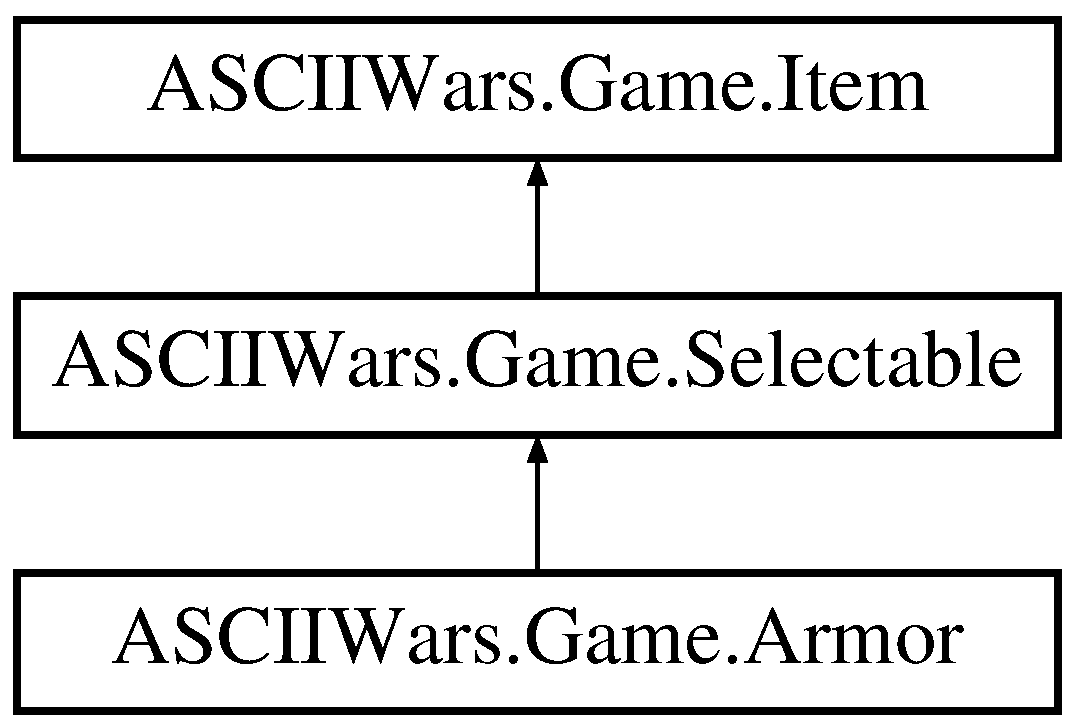
\includegraphics[height=3.000000cm]{class_a_s_c_i_i_wars_1_1_game_1_1_armor}
\end{center}
\end{figure}
\subsection*{Открытые члены}
\begin{DoxyCompactItemize}
\item 
\hyperlink{class_a_s_c_i_i_wars_1_1_game_1_1_armor_a3286b25da22682e4773667888ee99cf9}{Armor} (string \hyperlink{class_a_s_c_i_i_wars_1_1_game_1_1_item_a744d51f7684a4e46a1f834f8666db58e}{id}, string \hyperlink{class_a_s_c_i_i_wars_1_1_game_1_1_item_a994b9ec5f10c123e4345da159c090091}{name}, string \hyperlink{class_a_s_c_i_i_wars_1_1_game_1_1_item_a6ff41e953ccebc64a8df8f8c434535a0}{description}, int \hyperlink{class_a_s_c_i_i_wars_1_1_game_1_1_armor_ac056d4feeb6864656f00144af7a4ed8b}{defense})
\item 
override void \hyperlink{class_a_s_c_i_i_wars_1_1_game_1_1_armor_ab8e1364e91ddd19f7c214f051b054cd8}{On\+Add\+To\+Player\+Inventory} (\hyperlink{class_a_s_c_i_i_wars_1_1_game_1_1_player}{Player} player)
\item 
override void \hyperlink{class_a_s_c_i_i_wars_1_1_game_1_1_armor_ab4f8a39af009eef4bbdeb6db67fb9cd5}{On\+Select\+By\+Player} (\hyperlink{class_a_s_c_i_i_wars_1_1_game_1_1_player}{Player} player)
\item 
override void \hyperlink{class_a_s_c_i_i_wars_1_1_game_1_1_armor_af502379d334f2fc7901638f8a8eba130}{On\+Deselect\+By\+Player} (\hyperlink{class_a_s_c_i_i_wars_1_1_game_1_1_player}{Player} player)
\item 
override void \hyperlink{class_a_s_c_i_i_wars_1_1_game_1_1_armor_ab113733825094b12aba14b8b48372f9c}{On\+Remove\+From\+Player\+Inventory} (\hyperlink{class_a_s_c_i_i_wars_1_1_game_1_1_player}{Player} player)
\item 
override int \hyperlink{class_a_s_c_i_i_wars_1_1_game_1_1_armor_a7abccb710e5f53baf59b4184140d907e}{Get\+Hash\+Code} ()
\item 
override bool \hyperlink{class_a_s_c_i_i_wars_1_1_game_1_1_armor_a2cb86fcb3169af675628bd2ab7e00036}{Equals} (object obj)
\end{DoxyCompactItemize}
\subsection*{Открытые атрибуты}
\begin{DoxyCompactItemize}
\item 
readonly int \hyperlink{class_a_s_c_i_i_wars_1_1_game_1_1_armor_ac056d4feeb6864656f00144af7a4ed8b}{defense}
\end{DoxyCompactItemize}


\subsection{Конструктор(ы)}
\hypertarget{class_a_s_c_i_i_wars_1_1_game_1_1_armor_a3286b25da22682e4773667888ee99cf9}{}\label{class_a_s_c_i_i_wars_1_1_game_1_1_armor_a3286b25da22682e4773667888ee99cf9} 
\index{A\+S\+C\+I\+I\+Wars\+::\+Game\+::\+Armor@{A\+S\+C\+I\+I\+Wars\+::\+Game\+::\+Armor}!Armor@{Armor}}
\index{Armor@{Armor}!A\+S\+C\+I\+I\+Wars\+::\+Game\+::\+Armor@{A\+S\+C\+I\+I\+Wars\+::\+Game\+::\+Armor}}
\subsubsection{\texorpdfstring{Armor()}{Armor()}}
{\footnotesize\ttfamily A\+S\+C\+I\+I\+Wars.\+Game.\+Armor.\+Armor (\begin{DoxyParamCaption}\item[{string}]{id,  }\item[{string}]{name,  }\item[{string}]{description,  }\item[{int}]{defense }\end{DoxyParamCaption})\hspace{0.3cm}{\ttfamily [inline]}}



\subsection{Методы}
\hypertarget{class_a_s_c_i_i_wars_1_1_game_1_1_armor_a2cb86fcb3169af675628bd2ab7e00036}{}\label{class_a_s_c_i_i_wars_1_1_game_1_1_armor_a2cb86fcb3169af675628bd2ab7e00036} 
\index{A\+S\+C\+I\+I\+Wars\+::\+Game\+::\+Armor@{A\+S\+C\+I\+I\+Wars\+::\+Game\+::\+Armor}!Equals@{Equals}}
\index{Equals@{Equals}!A\+S\+C\+I\+I\+Wars\+::\+Game\+::\+Armor@{A\+S\+C\+I\+I\+Wars\+::\+Game\+::\+Armor}}
\subsubsection{\texorpdfstring{Equals()}{Equals()}}
{\footnotesize\ttfamily override bool A\+S\+C\+I\+I\+Wars.\+Game.\+Armor.\+Equals (\begin{DoxyParamCaption}\item[{object}]{obj }\end{DoxyParamCaption})\hspace{0.3cm}{\ttfamily [inline]}}

\hypertarget{class_a_s_c_i_i_wars_1_1_game_1_1_armor_a7abccb710e5f53baf59b4184140d907e}{}\label{class_a_s_c_i_i_wars_1_1_game_1_1_armor_a7abccb710e5f53baf59b4184140d907e} 
\index{A\+S\+C\+I\+I\+Wars\+::\+Game\+::\+Armor@{A\+S\+C\+I\+I\+Wars\+::\+Game\+::\+Armor}!Get\+Hash\+Code@{Get\+Hash\+Code}}
\index{Get\+Hash\+Code@{Get\+Hash\+Code}!A\+S\+C\+I\+I\+Wars\+::\+Game\+::\+Armor@{A\+S\+C\+I\+I\+Wars\+::\+Game\+::\+Armor}}
\subsubsection{\texorpdfstring{Get\+Hash\+Code()}{GetHashCode()}}
{\footnotesize\ttfamily override int A\+S\+C\+I\+I\+Wars.\+Game.\+Armor.\+Get\+Hash\+Code (\begin{DoxyParamCaption}{ }\end{DoxyParamCaption})\hspace{0.3cm}{\ttfamily [inline]}}

\hypertarget{class_a_s_c_i_i_wars_1_1_game_1_1_armor_ab8e1364e91ddd19f7c214f051b054cd8}{}\label{class_a_s_c_i_i_wars_1_1_game_1_1_armor_ab8e1364e91ddd19f7c214f051b054cd8} 
\index{A\+S\+C\+I\+I\+Wars\+::\+Game\+::\+Armor@{A\+S\+C\+I\+I\+Wars\+::\+Game\+::\+Armor}!On\+Add\+To\+Player\+Inventory@{On\+Add\+To\+Player\+Inventory}}
\index{On\+Add\+To\+Player\+Inventory@{On\+Add\+To\+Player\+Inventory}!A\+S\+C\+I\+I\+Wars\+::\+Game\+::\+Armor@{A\+S\+C\+I\+I\+Wars\+::\+Game\+::\+Armor}}
\subsubsection{\texorpdfstring{On\+Add\+To\+Player\+Inventory()}{OnAddToPlayerInventory()}}
{\footnotesize\ttfamily override void A\+S\+C\+I\+I\+Wars.\+Game.\+Armor.\+On\+Add\+To\+Player\+Inventory (\begin{DoxyParamCaption}\item[{\hyperlink{class_a_s_c_i_i_wars_1_1_game_1_1_player}{Player}}]{player }\end{DoxyParamCaption})\hspace{0.3cm}{\ttfamily [inline]}, {\ttfamily [virtual]}}



Замещает \hyperlink{class_a_s_c_i_i_wars_1_1_game_1_1_item_aec0355b7a9f647ef24897b95563f70d1}{A\+S\+C\+I\+I\+Wars.\+Game.\+Item}.

\hypertarget{class_a_s_c_i_i_wars_1_1_game_1_1_armor_af502379d334f2fc7901638f8a8eba130}{}\label{class_a_s_c_i_i_wars_1_1_game_1_1_armor_af502379d334f2fc7901638f8a8eba130} 
\index{A\+S\+C\+I\+I\+Wars\+::\+Game\+::\+Armor@{A\+S\+C\+I\+I\+Wars\+::\+Game\+::\+Armor}!On\+Deselect\+By\+Player@{On\+Deselect\+By\+Player}}
\index{On\+Deselect\+By\+Player@{On\+Deselect\+By\+Player}!A\+S\+C\+I\+I\+Wars\+::\+Game\+::\+Armor@{A\+S\+C\+I\+I\+Wars\+::\+Game\+::\+Armor}}
\subsubsection{\texorpdfstring{On\+Deselect\+By\+Player()}{OnDeselectByPlayer()}}
{\footnotesize\ttfamily override void A\+S\+C\+I\+I\+Wars.\+Game.\+Armor.\+On\+Deselect\+By\+Player (\begin{DoxyParamCaption}\item[{\hyperlink{class_a_s_c_i_i_wars_1_1_game_1_1_player}{Player}}]{player }\end{DoxyParamCaption})\hspace{0.3cm}{\ttfamily [inline]}, {\ttfamily [virtual]}}



Замещает \hyperlink{class_a_s_c_i_i_wars_1_1_game_1_1_selectable_a08a30c8786367bf45355e989b109c44b}{A\+S\+C\+I\+I\+Wars.\+Game.\+Selectable}.

\hypertarget{class_a_s_c_i_i_wars_1_1_game_1_1_armor_ab113733825094b12aba14b8b48372f9c}{}\label{class_a_s_c_i_i_wars_1_1_game_1_1_armor_ab113733825094b12aba14b8b48372f9c} 
\index{A\+S\+C\+I\+I\+Wars\+::\+Game\+::\+Armor@{A\+S\+C\+I\+I\+Wars\+::\+Game\+::\+Armor}!On\+Remove\+From\+Player\+Inventory@{On\+Remove\+From\+Player\+Inventory}}
\index{On\+Remove\+From\+Player\+Inventory@{On\+Remove\+From\+Player\+Inventory}!A\+S\+C\+I\+I\+Wars\+::\+Game\+::\+Armor@{A\+S\+C\+I\+I\+Wars\+::\+Game\+::\+Armor}}
\subsubsection{\texorpdfstring{On\+Remove\+From\+Player\+Inventory()}{OnRemoveFromPlayerInventory()}}
{\footnotesize\ttfamily override void A\+S\+C\+I\+I\+Wars.\+Game.\+Armor.\+On\+Remove\+From\+Player\+Inventory (\begin{DoxyParamCaption}\item[{\hyperlink{class_a_s_c_i_i_wars_1_1_game_1_1_player}{Player}}]{player }\end{DoxyParamCaption})\hspace{0.3cm}{\ttfamily [inline]}, {\ttfamily [virtual]}}



Замещает \hyperlink{class_a_s_c_i_i_wars_1_1_game_1_1_item_a52412546f837bfc65a3aa9d728fa142f}{A\+S\+C\+I\+I\+Wars.\+Game.\+Item}.

\hypertarget{class_a_s_c_i_i_wars_1_1_game_1_1_armor_ab4f8a39af009eef4bbdeb6db67fb9cd5}{}\label{class_a_s_c_i_i_wars_1_1_game_1_1_armor_ab4f8a39af009eef4bbdeb6db67fb9cd5} 
\index{A\+S\+C\+I\+I\+Wars\+::\+Game\+::\+Armor@{A\+S\+C\+I\+I\+Wars\+::\+Game\+::\+Armor}!On\+Select\+By\+Player@{On\+Select\+By\+Player}}
\index{On\+Select\+By\+Player@{On\+Select\+By\+Player}!A\+S\+C\+I\+I\+Wars\+::\+Game\+::\+Armor@{A\+S\+C\+I\+I\+Wars\+::\+Game\+::\+Armor}}
\subsubsection{\texorpdfstring{On\+Select\+By\+Player()}{OnSelectByPlayer()}}
{\footnotesize\ttfamily override void A\+S\+C\+I\+I\+Wars.\+Game.\+Armor.\+On\+Select\+By\+Player (\begin{DoxyParamCaption}\item[{\hyperlink{class_a_s_c_i_i_wars_1_1_game_1_1_player}{Player}}]{player }\end{DoxyParamCaption})\hspace{0.3cm}{\ttfamily [inline]}, {\ttfamily [virtual]}}



Замещает \hyperlink{class_a_s_c_i_i_wars_1_1_game_1_1_selectable_a95bdcf05ef9ea5f39c81ddd96294968a}{A\+S\+C\+I\+I\+Wars.\+Game.\+Selectable}.



\subsection{Данные класса}
\hypertarget{class_a_s_c_i_i_wars_1_1_game_1_1_armor_ac056d4feeb6864656f00144af7a4ed8b}{}\label{class_a_s_c_i_i_wars_1_1_game_1_1_armor_ac056d4feeb6864656f00144af7a4ed8b} 
\index{A\+S\+C\+I\+I\+Wars\+::\+Game\+::\+Armor@{A\+S\+C\+I\+I\+Wars\+::\+Game\+::\+Armor}!defense@{defense}}
\index{defense@{defense}!A\+S\+C\+I\+I\+Wars\+::\+Game\+::\+Armor@{A\+S\+C\+I\+I\+Wars\+::\+Game\+::\+Armor}}
\subsubsection{\texorpdfstring{defense}{defense}}
{\footnotesize\ttfamily readonly int A\+S\+C\+I\+I\+Wars.\+Game.\+Armor.\+defense}



Объявления и описания членов класса находятся в файле\+:\begin{DoxyCompactItemize}
\item 
Game/\hyperlink{_player_8cs}{Player.\+cs}\end{DoxyCompactItemize}

\hypertarget{class_a_s_c_i_i_wars_1_1_game_1_1_asset}{}\section{Класс A\+S\+C\+I\+I\+Wars.\+Game.\+Asset}
\label{class_a_s_c_i_i_wars_1_1_game_1_1_asset}\index{A\+S\+C\+I\+I\+Wars.\+Game.\+Asset@{A\+S\+C\+I\+I\+Wars.\+Game.\+Asset}}


Ассет. Хранит текст ассета.  


\subsection*{Открытые члены}
\begin{DoxyCompactItemize}
\item 
\hypertarget{class_a_s_c_i_i_wars_1_1_game_1_1_asset_ab587d66e5e4257ab6baa804b00f2b112}{}\label{class_a_s_c_i_i_wars_1_1_game_1_1_asset_ab587d66e5e4257ab6baa804b00f2b112} 
{\bfseries Asset} (string assets\+Directory, string group\+Name, string name)
\item 
\hypertarget{class_a_s_c_i_i_wars_1_1_game_1_1_asset_aaf8fcd0eea1ca1b6a5cd26be7ee8c24c}{}\label{class_a_s_c_i_i_wars_1_1_game_1_1_asset_aaf8fcd0eea1ca1b6a5cd26be7ee8c24c} 
override string {\bfseries To\+String} ()
\end{DoxyCompactItemize}
\subsection*{Открытые атрибуты}
\begin{DoxyCompactItemize}
\item 
\hypertarget{class_a_s_c_i_i_wars_1_1_game_1_1_asset_ac77e5c7b34bf76f64cc56e2519e4ef10}{}\label{class_a_s_c_i_i_wars_1_1_game_1_1_asset_ac77e5c7b34bf76f64cc56e2519e4ef10} 
readonly string {\bfseries assets\+Directory}
\item 
\hypertarget{class_a_s_c_i_i_wars_1_1_game_1_1_asset_abdde541a3e0a35d1f80de3ceaea7db50}{}\label{class_a_s_c_i_i_wars_1_1_game_1_1_asset_abdde541a3e0a35d1f80de3ceaea7db50} 
readonly string {\bfseries group\+Name}
\item 
\hypertarget{class_a_s_c_i_i_wars_1_1_game_1_1_asset_a5bd9f716708c7943bdd313357da7d7f3}{}\label{class_a_s_c_i_i_wars_1_1_game_1_1_asset_a5bd9f716708c7943bdd313357da7d7f3} 
readonly string {\bfseries name}
\item 
\hypertarget{class_a_s_c_i_i_wars_1_1_game_1_1_asset_a2d1d00016592f2930725bf14a2a05fb8}{}\label{class_a_s_c_i_i_wars_1_1_game_1_1_asset_a2d1d00016592f2930725bf14a2a05fb8} 
readonly string {\bfseries path}
\item 
\hypertarget{class_a_s_c_i_i_wars_1_1_game_1_1_asset_a6be81140383341818eaea6ffd8c6c29b}{}\label{class_a_s_c_i_i_wars_1_1_game_1_1_asset_a6be81140383341818eaea6ffd8c6c29b} 
readonly string {\bfseries content}
\item 
\hypertarget{class_a_s_c_i_i_wars_1_1_game_1_1_asset_ab69cdc626d285fd7e8415f0b7cb25f54}{}\label{class_a_s_c_i_i_wars_1_1_game_1_1_asset_ab69cdc626d285fd7e8415f0b7cb25f54} 
readonly string \mbox{[}$\,$\mbox{]} {\bfseries lines}
\end{DoxyCompactItemize}


\subsection{Подробное описание}
Ассет. Хранит текст ассета. 

\begin{DoxySeeAlso}{См. также}
\hyperlink{class_a_s_c_i_i_wars_1_1_game_1_1_asset_container}{Asset\+Container} 

\hyperlink{class_a_s_c_i_i_wars_1_1_game_1_1_asset_group}{Asset\+Group} 
\end{DoxySeeAlso}


Объявления и описания членов класса находятся в файле\+:\begin{DoxyCompactItemize}
\item 
A\+S\+C\+I\+I\+Wars/\+Game/Assets.\+cs\end{DoxyCompactItemize}

\hypertarget{class_a_s_c_i_i_wars_1_1_game_1_1_asset_container}{}\section{Класс A\+S\+C\+I\+I\+Wars.\+Game.\+Asset\+Container}
\label{class_a_s_c_i_i_wars_1_1_game_1_1_asset_container}\index{A\+S\+C\+I\+I\+Wars.\+Game.\+Asset\+Container@{A\+S\+C\+I\+I\+Wars.\+Game.\+Asset\+Container}}


Контейнер ассетов. Хранит их по групам. В каждой группе находятся файлы ассетов.  


\subsection*{Открытые члены}
\begin{DoxyCompactItemize}
\item 
\hyperlink{class_a_s_c_i_i_wars_1_1_game_1_1_asset_container_afb55a3f711d67504b677fc2bc38718cc}{Asset\+Container} (string assets\+Directory)
\item 
\hypertarget{class_a_s_c_i_i_wars_1_1_game_1_1_asset_container_a73cb91685f397df31d2a18d8b59b3093}{}\label{class_a_s_c_i_i_wars_1_1_game_1_1_asset_container_a73cb91685f397df31d2a18d8b59b3093} 
override string {\bfseries To\+String} ()
\end{DoxyCompactItemize}
\subsection*{Открытые атрибуты}
\begin{DoxyCompactItemize}
\item 
\hypertarget{class_a_s_c_i_i_wars_1_1_game_1_1_asset_container_afc2c4d42edc386fa6bdbf561546b2083}{}\label{class_a_s_c_i_i_wars_1_1_game_1_1_asset_container_afc2c4d42edc386fa6bdbf561546b2083} 
readonly Dictionary$<$ string, \hyperlink{class_a_s_c_i_i_wars_1_1_game_1_1_asset_group}{Asset\+Group} $>$ {\bfseries asset\+Groups} = new Dictionary$<$string, \hyperlink{class_a_s_c_i_i_wars_1_1_game_1_1_asset_group}{Asset\+Group}$>$()
\end{DoxyCompactItemize}
\subsection*{Свойства}
\begin{DoxyCompactItemize}
\item 
\hypertarget{class_a_s_c_i_i_wars_1_1_game_1_1_asset_container_ae7149eab74d76098eca27b20d49d0bf9}{}\label{class_a_s_c_i_i_wars_1_1_game_1_1_asset_container_ae7149eab74d76098eca27b20d49d0bf9} 
\hyperlink{class_a_s_c_i_i_wars_1_1_game_1_1_asset_group}{Asset\+Group} {\bfseries this\mbox{[}string group\+Name\mbox{]}}\hspace{0.3cm}{\ttfamily  \mbox{[}get, set\mbox{]}}
\end{DoxyCompactItemize}


\subsection{Подробное описание}
Контейнер ассетов. Хранит их по групам. В каждой группе находятся файлы ассетов. 

В представлении файловой системы выглядит так\+: 
\begin{DoxyCode}
> assetsDirectory/
>     assetGroup1/
>         asset1.txt
>         asset2.json
>     assetGroup2/
>         asset1.png
>         asset2.mp3
\end{DoxyCode}


\begin{DoxySeeAlso}{См. также}
\hyperlink{class_a_s_c_i_i_wars_1_1_game_1_1_asset_group}{Asset\+Group} 

\hyperlink{class_a_s_c_i_i_wars_1_1_game_1_1_asset}{Asset} 
\end{DoxySeeAlso}


\subsection{Конструктор(ы)}
\hypertarget{class_a_s_c_i_i_wars_1_1_game_1_1_asset_container_afb55a3f711d67504b677fc2bc38718cc}{}\label{class_a_s_c_i_i_wars_1_1_game_1_1_asset_container_afb55a3f711d67504b677fc2bc38718cc} 
\index{A\+S\+C\+I\+I\+Wars\+::\+Game\+::\+Asset\+Container@{A\+S\+C\+I\+I\+Wars\+::\+Game\+::\+Asset\+Container}!Asset\+Container@{Asset\+Container}}
\index{Asset\+Container@{Asset\+Container}!A\+S\+C\+I\+I\+Wars\+::\+Game\+::\+Asset\+Container@{A\+S\+C\+I\+I\+Wars\+::\+Game\+::\+Asset\+Container}}
\subsubsection{\texorpdfstring{Asset\+Container()}{AssetContainer()}}
{\footnotesize\ttfamily A\+S\+C\+I\+I\+Wars.\+Game.\+Asset\+Container.\+Asset\+Container (\begin{DoxyParamCaption}\item[{string}]{assets\+Directory }\end{DoxyParamCaption})\hspace{0.3cm}{\ttfamily [inline]}}

Инициализирует контейнер с указанем деректории, откуда грузить группы ассетов. 

Объявления и описания членов класса находятся в файле\+:\begin{DoxyCompactItemize}
\item 
A\+S\+C\+I\+I\+Wars/\+Game/Assets.\+cs\end{DoxyCompactItemize}

\hypertarget{class_a_s_c_i_i_wars_1_1_game_1_1_asset_group}{}\section{Класс A\+S\+C\+I\+I\+Wars.\+Game.\+Asset\+Group}
\label{class_a_s_c_i_i_wars_1_1_game_1_1_asset_group}\index{A\+S\+C\+I\+I\+Wars.\+Game.\+Asset\+Group@{A\+S\+C\+I\+I\+Wars.\+Game.\+Asset\+Group}}


Хранит файлы с ассетами.  


\subsection*{Открытые члены}
\begin{DoxyCompactItemize}
\item 
\hyperlink{class_a_s_c_i_i_wars_1_1_game_1_1_asset_group_a0477f5fe9d3a2828e2ef4c2ddb7aa565}{Asset\+Group} (string \hyperlink{class_a_s_c_i_i_wars_1_1_game_1_1_asset_group_a6c7083ec7602a32f4e99601ef5d54397}{assets\+Directory}, string \hyperlink{class_a_s_c_i_i_wars_1_1_game_1_1_asset_group_aeb6e4bd616bf065ce4a04f5c34e9c3d9}{name}, Dictionary$<$ string, \hyperlink{class_a_s_c_i_i_wars_1_1_game_1_1_asset}{Asset} $>$ \hyperlink{class_a_s_c_i_i_wars_1_1_game_1_1_asset_group_ae2481944ac1b6ebe0f4e383ef7de141c}{assets})
\item 
override string \hyperlink{class_a_s_c_i_i_wars_1_1_game_1_1_asset_group_a16cbe328487eba763e92bb4551a67311}{To\+String} ()
\end{DoxyCompactItemize}
\subsection*{Открытые атрибуты}
\begin{DoxyCompactItemize}
\item 
readonly string \hyperlink{class_a_s_c_i_i_wars_1_1_game_1_1_asset_group_a6c7083ec7602a32f4e99601ef5d54397}{assets\+Directory}
\item 
readonly string \hyperlink{class_a_s_c_i_i_wars_1_1_game_1_1_asset_group_aeb6e4bd616bf065ce4a04f5c34e9c3d9}{name}
\item 
readonly Dictionary$<$ string, \hyperlink{class_a_s_c_i_i_wars_1_1_game_1_1_asset}{Asset} $>$ \hyperlink{class_a_s_c_i_i_wars_1_1_game_1_1_asset_group_ae2481944ac1b6ebe0f4e383ef7de141c}{assets}
\end{DoxyCompactItemize}
\subsection*{Свойства}
\begin{DoxyCompactItemize}
\item 
\hyperlink{class_a_s_c_i_i_wars_1_1_game_1_1_asset}{Asset} \hyperlink{class_a_s_c_i_i_wars_1_1_game_1_1_asset_group_ada6ec78bb13c41b4f8309f91b4adeecc}{this\mbox{[}string asset\+Name\mbox{]}}\hspace{0.3cm}{\ttfamily  \mbox{[}get, set\mbox{]}}
\end{DoxyCompactItemize}


\subsection{Подробное описание}
Хранит файлы с ассетами. 

В представлении файловой системы выглядит так\+: 
\begin{DoxyCode}
\hyperlink{class_a_s_c_i_i_wars_1_1_game_1_1_asset_group_a6c7083ec7602a32f4e99601ef5d54397}{assetsDirectory}/
>     assetGroup1/
>         asset1.txt
>         asset2.json
    assetGroup2/
        asset1.png
        asset2.mp3
\end{DoxyCode}


\begin{DoxySeeAlso}{См. также}
\hyperlink{class_a_s_c_i_i_wars_1_1_game_1_1_asset_container}{Asset\+Container} 

\hyperlink{class_a_s_c_i_i_wars_1_1_game_1_1_asset}{Asset} 
\end{DoxySeeAlso}


\subsection{Конструктор(ы)}
\hypertarget{class_a_s_c_i_i_wars_1_1_game_1_1_asset_group_a0477f5fe9d3a2828e2ef4c2ddb7aa565}{}\label{class_a_s_c_i_i_wars_1_1_game_1_1_asset_group_a0477f5fe9d3a2828e2ef4c2ddb7aa565} 
\index{A\+S\+C\+I\+I\+Wars\+::\+Game\+::\+Asset\+Group@{A\+S\+C\+I\+I\+Wars\+::\+Game\+::\+Asset\+Group}!Asset\+Group@{Asset\+Group}}
\index{Asset\+Group@{Asset\+Group}!A\+S\+C\+I\+I\+Wars\+::\+Game\+::\+Asset\+Group@{A\+S\+C\+I\+I\+Wars\+::\+Game\+::\+Asset\+Group}}
\subsubsection{\texorpdfstring{Asset\+Group()}{AssetGroup()}}
{\footnotesize\ttfamily A\+S\+C\+I\+I\+Wars.\+Game.\+Asset\+Group.\+Asset\+Group (\begin{DoxyParamCaption}\item[{string}]{assets\+Directory,  }\item[{string}]{name,  }\item[{Dictionary$<$ string, \hyperlink{class_a_s_c_i_i_wars_1_1_game_1_1_asset}{Asset} $>$}]{assets }\end{DoxyParamCaption})\hspace{0.3cm}{\ttfamily [inline]}}



\subsection{Методы}
\hypertarget{class_a_s_c_i_i_wars_1_1_game_1_1_asset_group_a16cbe328487eba763e92bb4551a67311}{}\label{class_a_s_c_i_i_wars_1_1_game_1_1_asset_group_a16cbe328487eba763e92bb4551a67311} 
\index{A\+S\+C\+I\+I\+Wars\+::\+Game\+::\+Asset\+Group@{A\+S\+C\+I\+I\+Wars\+::\+Game\+::\+Asset\+Group}!To\+String@{To\+String}}
\index{To\+String@{To\+String}!A\+S\+C\+I\+I\+Wars\+::\+Game\+::\+Asset\+Group@{A\+S\+C\+I\+I\+Wars\+::\+Game\+::\+Asset\+Group}}
\subsubsection{\texorpdfstring{To\+String()}{ToString()}}
{\footnotesize\ttfamily override string A\+S\+C\+I\+I\+Wars.\+Game.\+Asset\+Group.\+To\+String (\begin{DoxyParamCaption}{ }\end{DoxyParamCaption})\hspace{0.3cm}{\ttfamily [inline]}}



\subsection{Данные класса}
\hypertarget{class_a_s_c_i_i_wars_1_1_game_1_1_asset_group_ae2481944ac1b6ebe0f4e383ef7de141c}{}\label{class_a_s_c_i_i_wars_1_1_game_1_1_asset_group_ae2481944ac1b6ebe0f4e383ef7de141c} 
\index{A\+S\+C\+I\+I\+Wars\+::\+Game\+::\+Asset\+Group@{A\+S\+C\+I\+I\+Wars\+::\+Game\+::\+Asset\+Group}!assets@{assets}}
\index{assets@{assets}!A\+S\+C\+I\+I\+Wars\+::\+Game\+::\+Asset\+Group@{A\+S\+C\+I\+I\+Wars\+::\+Game\+::\+Asset\+Group}}
\subsubsection{\texorpdfstring{assets}{assets}}
{\footnotesize\ttfamily readonly Dictionary$<$string, \hyperlink{class_a_s_c_i_i_wars_1_1_game_1_1_asset}{Asset}$>$ A\+S\+C\+I\+I\+Wars.\+Game.\+Asset\+Group.\+assets}

\hypertarget{class_a_s_c_i_i_wars_1_1_game_1_1_asset_group_a6c7083ec7602a32f4e99601ef5d54397}{}\label{class_a_s_c_i_i_wars_1_1_game_1_1_asset_group_a6c7083ec7602a32f4e99601ef5d54397} 
\index{A\+S\+C\+I\+I\+Wars\+::\+Game\+::\+Asset\+Group@{A\+S\+C\+I\+I\+Wars\+::\+Game\+::\+Asset\+Group}!assets\+Directory@{assets\+Directory}}
\index{assets\+Directory@{assets\+Directory}!A\+S\+C\+I\+I\+Wars\+::\+Game\+::\+Asset\+Group@{A\+S\+C\+I\+I\+Wars\+::\+Game\+::\+Asset\+Group}}
\subsubsection{\texorpdfstring{assets\+Directory}{assetsDirectory}}
{\footnotesize\ttfamily readonly string A\+S\+C\+I\+I\+Wars.\+Game.\+Asset\+Group.\+assets\+Directory}

\hypertarget{class_a_s_c_i_i_wars_1_1_game_1_1_asset_group_aeb6e4bd616bf065ce4a04f5c34e9c3d9}{}\label{class_a_s_c_i_i_wars_1_1_game_1_1_asset_group_aeb6e4bd616bf065ce4a04f5c34e9c3d9} 
\index{A\+S\+C\+I\+I\+Wars\+::\+Game\+::\+Asset\+Group@{A\+S\+C\+I\+I\+Wars\+::\+Game\+::\+Asset\+Group}!name@{name}}
\index{name@{name}!A\+S\+C\+I\+I\+Wars\+::\+Game\+::\+Asset\+Group@{A\+S\+C\+I\+I\+Wars\+::\+Game\+::\+Asset\+Group}}
\subsubsection{\texorpdfstring{name}{name}}
{\footnotesize\ttfamily readonly string A\+S\+C\+I\+I\+Wars.\+Game.\+Asset\+Group.\+name}



\subsection{Полный список свойств}
\hypertarget{class_a_s_c_i_i_wars_1_1_game_1_1_asset_group_ada6ec78bb13c41b4f8309f91b4adeecc}{}\label{class_a_s_c_i_i_wars_1_1_game_1_1_asset_group_ada6ec78bb13c41b4f8309f91b4adeecc} 
\index{A\+S\+C\+I\+I\+Wars\+::\+Game\+::\+Asset\+Group@{A\+S\+C\+I\+I\+Wars\+::\+Game\+::\+Asset\+Group}!this\mbox{[}string asset\+Name\mbox{]}@{this[string asset\+Name]}}
\index{this\mbox{[}string asset\+Name\mbox{]}@{this[string asset\+Name]}!A\+S\+C\+I\+I\+Wars\+::\+Game\+::\+Asset\+Group@{A\+S\+C\+I\+I\+Wars\+::\+Game\+::\+Asset\+Group}}
\subsubsection{\texorpdfstring{this[string asset\+Name]}{this[string assetName]}}
{\footnotesize\ttfamily \hyperlink{class_a_s_c_i_i_wars_1_1_game_1_1_asset}{Asset} A\+S\+C\+I\+I\+Wars.\+Game.\+Asset\+Group.\+this\mbox{[}string asset\+Name\mbox{]}\hspace{0.3cm}{\ttfamily [get]}, {\ttfamily [set]}}



Объявления и описания членов класса находятся в файле\+:\begin{DoxyCompactItemize}
\item 
A\+S\+C\+I\+I\+Wars/\+Game/\hyperlink{_assets_8cs}{Assets.\+cs}\end{DoxyCompactItemize}

\hypertarget{class_a_s_c_i_i_wars_1_1_game_1_1_branch}{}\section{Класс A\+S\+C\+I\+I\+Wars.\+Game.\+Branch}
\label{class_a_s_c_i_i_wars_1_1_game_1_1_branch}\index{A\+S\+C\+I\+I\+Wars.\+Game.\+Branch@{A\+S\+C\+I\+I\+Wars.\+Game.\+Branch}}
\subsection*{Открытые атрибуты}
\begin{DoxyCompactItemize}
\item 
string \hyperlink{class_a_s_c_i_i_wars_1_1_game_1_1_branch_a1282f409f0d3f4920253079ed5f2ba3c}{id}
\item 
string \hyperlink{class_a_s_c_i_i_wars_1_1_game_1_1_branch_aa1a7fc6d8ff84881ecea850ef481616d}{title}
\item 
List$<$ \hyperlink{class_a_s_c_i_i_wars_1_1_game_1_1_next_situation}{Next\+Situation} $>$ \hyperlink{class_a_s_c_i_i_wars_1_1_game_1_1_branch_a1f68675102e4e66e210874145273522c}{next\+Situations}
\end{DoxyCompactItemize}


\subsection{Данные класса}
\hypertarget{class_a_s_c_i_i_wars_1_1_game_1_1_branch_a1282f409f0d3f4920253079ed5f2ba3c}{}\label{class_a_s_c_i_i_wars_1_1_game_1_1_branch_a1282f409f0d3f4920253079ed5f2ba3c} 
\index{A\+S\+C\+I\+I\+Wars\+::\+Game\+::\+Branch@{A\+S\+C\+I\+I\+Wars\+::\+Game\+::\+Branch}!id@{id}}
\index{id@{id}!A\+S\+C\+I\+I\+Wars\+::\+Game\+::\+Branch@{A\+S\+C\+I\+I\+Wars\+::\+Game\+::\+Branch}}
\subsubsection{\texorpdfstring{id}{id}}
{\footnotesize\ttfamily string A\+S\+C\+I\+I\+Wars.\+Game.\+Branch.\+id}

\hypertarget{class_a_s_c_i_i_wars_1_1_game_1_1_branch_a1f68675102e4e66e210874145273522c}{}\label{class_a_s_c_i_i_wars_1_1_game_1_1_branch_a1f68675102e4e66e210874145273522c} 
\index{A\+S\+C\+I\+I\+Wars\+::\+Game\+::\+Branch@{A\+S\+C\+I\+I\+Wars\+::\+Game\+::\+Branch}!next\+Situations@{next\+Situations}}
\index{next\+Situations@{next\+Situations}!A\+S\+C\+I\+I\+Wars\+::\+Game\+::\+Branch@{A\+S\+C\+I\+I\+Wars\+::\+Game\+::\+Branch}}
\subsubsection{\texorpdfstring{next\+Situations}{nextSituations}}
{\footnotesize\ttfamily List$<$\hyperlink{class_a_s_c_i_i_wars_1_1_game_1_1_next_situation}{Next\+Situation}$>$ A\+S\+C\+I\+I\+Wars.\+Game.\+Branch.\+next\+Situations}

\hypertarget{class_a_s_c_i_i_wars_1_1_game_1_1_branch_aa1a7fc6d8ff84881ecea850ef481616d}{}\label{class_a_s_c_i_i_wars_1_1_game_1_1_branch_aa1a7fc6d8ff84881ecea850ef481616d} 
\index{A\+S\+C\+I\+I\+Wars\+::\+Game\+::\+Branch@{A\+S\+C\+I\+I\+Wars\+::\+Game\+::\+Branch}!title@{title}}
\index{title@{title}!A\+S\+C\+I\+I\+Wars\+::\+Game\+::\+Branch@{A\+S\+C\+I\+I\+Wars\+::\+Game\+::\+Branch}}
\subsubsection{\texorpdfstring{title}{title}}
{\footnotesize\ttfamily string A\+S\+C\+I\+I\+Wars.\+Game.\+Branch.\+title}



Объявления и описания членов класса находятся в файле\+:\begin{DoxyCompactItemize}
\item 
A\+S\+C\+I\+I\+Wars/\+Game/\hyperlink{_situations_8cs}{Situations.\+cs}\end{DoxyCompactItemize}

\hypertarget{class_a_s_c_i_i_wars_1_1_game_1_1_consumable}{}\section{Класс A\+S\+C\+I\+I\+Wars.\+Game.\+Consumable}
\label{class_a_s_c_i_i_wars_1_1_game_1_1_consumable}\index{A\+S\+C\+I\+I\+Wars.\+Game.\+Consumable@{A\+S\+C\+I\+I\+Wars.\+Game.\+Consumable}}
Граф наследования\+:A\+S\+C\+I\+I\+Wars.\+Game.\+Consumable\+:\begin{figure}[H]
\begin{center}
\leavevmode
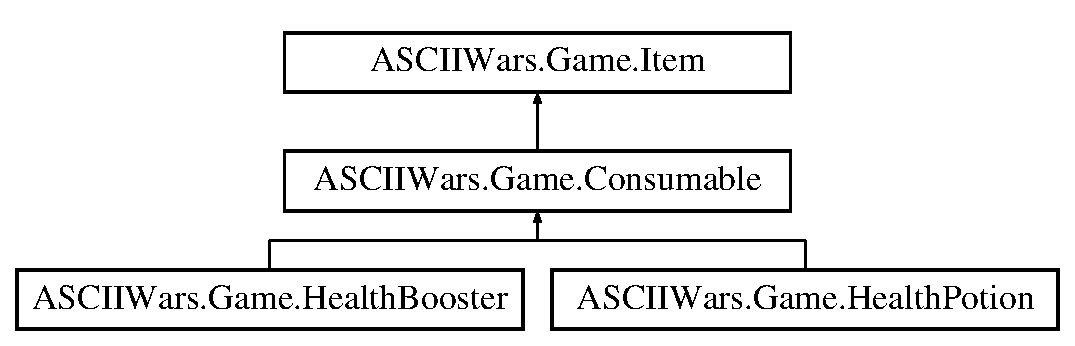
\includegraphics[height=3.000000cm]{class_a_s_c_i_i_wars_1_1_game_1_1_consumable}
\end{center}
\end{figure}
\subsection*{Открытые члены}
\begin{DoxyCompactItemize}
\item 
\hyperlink{class_a_s_c_i_i_wars_1_1_game_1_1_consumable_aa445dfd287fc22cfb76b133614fec0c2}{Consumable} (string \hyperlink{class_a_s_c_i_i_wars_1_1_game_1_1_item_a744d51f7684a4e46a1f834f8666db58e}{id}, string \hyperlink{class_a_s_c_i_i_wars_1_1_game_1_1_item_a994b9ec5f10c123e4345da159c090091}{name}, string \hyperlink{class_a_s_c_i_i_wars_1_1_game_1_1_item_a6ff41e953ccebc64a8df8f8c434535a0}{description})
\item 
abstract void \hyperlink{class_a_s_c_i_i_wars_1_1_game_1_1_consumable_a6aac67fe076ca39cb850e3720461fff8}{On\+Consume\+By\+Player} (\hyperlink{class_a_s_c_i_i_wars_1_1_game_1_1_player}{Player} player)
\end{DoxyCompactItemize}
\subsection*{Дополнительные унаследованные члены}


\subsection{Конструктор(ы)}
\hypertarget{class_a_s_c_i_i_wars_1_1_game_1_1_consumable_aa445dfd287fc22cfb76b133614fec0c2}{}\label{class_a_s_c_i_i_wars_1_1_game_1_1_consumable_aa445dfd287fc22cfb76b133614fec0c2} 
\index{A\+S\+C\+I\+I\+Wars\+::\+Game\+::\+Consumable@{A\+S\+C\+I\+I\+Wars\+::\+Game\+::\+Consumable}!Consumable@{Consumable}}
\index{Consumable@{Consumable}!A\+S\+C\+I\+I\+Wars\+::\+Game\+::\+Consumable@{A\+S\+C\+I\+I\+Wars\+::\+Game\+::\+Consumable}}
\subsubsection{\texorpdfstring{Consumable()}{Consumable()}}
{\footnotesize\ttfamily A\+S\+C\+I\+I\+Wars.\+Game.\+Consumable.\+Consumable (\begin{DoxyParamCaption}\item[{string}]{id,  }\item[{string}]{name,  }\item[{string}]{description }\end{DoxyParamCaption})\hspace{0.3cm}{\ttfamily [inline]}}



\subsection{Методы}
\hypertarget{class_a_s_c_i_i_wars_1_1_game_1_1_consumable_a6aac67fe076ca39cb850e3720461fff8}{}\label{class_a_s_c_i_i_wars_1_1_game_1_1_consumable_a6aac67fe076ca39cb850e3720461fff8} 
\index{A\+S\+C\+I\+I\+Wars\+::\+Game\+::\+Consumable@{A\+S\+C\+I\+I\+Wars\+::\+Game\+::\+Consumable}!On\+Consume\+By\+Player@{On\+Consume\+By\+Player}}
\index{On\+Consume\+By\+Player@{On\+Consume\+By\+Player}!A\+S\+C\+I\+I\+Wars\+::\+Game\+::\+Consumable@{A\+S\+C\+I\+I\+Wars\+::\+Game\+::\+Consumable}}
\subsubsection{\texorpdfstring{On\+Consume\+By\+Player()}{OnConsumeByPlayer()}}
{\footnotesize\ttfamily abstract void A\+S\+C\+I\+I\+Wars.\+Game.\+Consumable.\+On\+Consume\+By\+Player (\begin{DoxyParamCaption}\item[{\hyperlink{class_a_s_c_i_i_wars_1_1_game_1_1_player}{Player}}]{player }\end{DoxyParamCaption})\hspace{0.3cm}{\ttfamily [pure virtual]}}



Замещается в \hyperlink{class_a_s_c_i_i_wars_1_1_game_1_1_health_booster_a0dd6134e102b2b4ea9d143b7cea15568}{A\+S\+C\+I\+I\+Wars.\+Game.\+Health\+Booster} и \hyperlink{class_a_s_c_i_i_wars_1_1_game_1_1_health_potion_a3004d1c2396e9c068ed4e03884afd56c}{A\+S\+C\+I\+I\+Wars.\+Game.\+Health\+Potion}.



Объявления и описания членов класса находятся в файле\+:\begin{DoxyCompactItemize}
\item 
Game/\hyperlink{_player_8cs}{Player.\+cs}\end{DoxyCompactItemize}

\hypertarget{class_a_s_c_i_i_wars_1_1_game_1_1_craft}{}\section{Класс A\+S\+C\+I\+I\+Wars.\+Game.\+Craft}
\label{class_a_s_c_i_i_wars_1_1_game_1_1_craft}\index{A\+S\+C\+I\+I\+Wars.\+Game.\+Craft@{A\+S\+C\+I\+I\+Wars.\+Game.\+Craft}}
\subsection*{Открытые атрибуты}
\begin{DoxyCompactItemize}
\item 
\hypertarget{class_a_s_c_i_i_wars_1_1_game_1_1_craft_aece38d819ddd8edebf172db5bdd1f13b}{}\label{class_a_s_c_i_i_wars_1_1_game_1_1_craft_aece38d819ddd8edebf172db5bdd1f13b} 
List$<$ \hyperlink{class_a_s_c_i_i_wars_1_1_game_1_1_crafting_item}{Crafting\+Item} $>$ {\bfseries ingredients}
\item 
\hypertarget{class_a_s_c_i_i_wars_1_1_game_1_1_craft_ae7a24959d740187fde0bf8df00691522}{}\label{class_a_s_c_i_i_wars_1_1_game_1_1_craft_ae7a24959d740187fde0bf8df00691522} 
\hyperlink{class_a_s_c_i_i_wars_1_1_game_1_1_crafting_item}{Crafting\+Item} {\bfseries result}
\end{DoxyCompactItemize}


Объявления и описания членов класса находятся в файле\+:\begin{DoxyCompactItemize}
\item 
A\+S\+C\+I\+I\+Wars/\+Game/Situations.\+cs\end{DoxyCompactItemize}

\hypertarget{class_a_s_c_i_i_wars_1_1_game_1_1_crafting_item}{}\section{Класс A\+S\+C\+I\+I\+Wars.\+Game.\+Crafting\+Item}
\label{class_a_s_c_i_i_wars_1_1_game_1_1_crafting_item}\index{A\+S\+C\+I\+I\+Wars.\+Game.\+Crafting\+Item@{A\+S\+C\+I\+I\+Wars.\+Game.\+Crafting\+Item}}
\subsection*{Открытые атрибуты}
\begin{DoxyCompactItemize}
\item 
string \hyperlink{class_a_s_c_i_i_wars_1_1_game_1_1_crafting_item_a053928c27417f2ff248fae79f1e5adc3}{id}
\item 
string \hyperlink{class_a_s_c_i_i_wars_1_1_game_1_1_crafting_item_a18242bdb01042b4a85c92fdb3bff0d05}{type}
\item 
int \hyperlink{class_a_s_c_i_i_wars_1_1_game_1_1_crafting_item_af27ae0339fb398e1e2a8d554c7909630}{count}
\end{DoxyCompactItemize}


\subsection{Данные класса}
\hypertarget{class_a_s_c_i_i_wars_1_1_game_1_1_crafting_item_af27ae0339fb398e1e2a8d554c7909630}{}\label{class_a_s_c_i_i_wars_1_1_game_1_1_crafting_item_af27ae0339fb398e1e2a8d554c7909630} 
\index{A\+S\+C\+I\+I\+Wars\+::\+Game\+::\+Crafting\+Item@{A\+S\+C\+I\+I\+Wars\+::\+Game\+::\+Crafting\+Item}!count@{count}}
\index{count@{count}!A\+S\+C\+I\+I\+Wars\+::\+Game\+::\+Crafting\+Item@{A\+S\+C\+I\+I\+Wars\+::\+Game\+::\+Crafting\+Item}}
\subsubsection{\texorpdfstring{count}{count}}
{\footnotesize\ttfamily int A\+S\+C\+I\+I\+Wars.\+Game.\+Crafting\+Item.\+count}

\hypertarget{class_a_s_c_i_i_wars_1_1_game_1_1_crafting_item_a053928c27417f2ff248fae79f1e5adc3}{}\label{class_a_s_c_i_i_wars_1_1_game_1_1_crafting_item_a053928c27417f2ff248fae79f1e5adc3} 
\index{A\+S\+C\+I\+I\+Wars\+::\+Game\+::\+Crafting\+Item@{A\+S\+C\+I\+I\+Wars\+::\+Game\+::\+Crafting\+Item}!id@{id}}
\index{id@{id}!A\+S\+C\+I\+I\+Wars\+::\+Game\+::\+Crafting\+Item@{A\+S\+C\+I\+I\+Wars\+::\+Game\+::\+Crafting\+Item}}
\subsubsection{\texorpdfstring{id}{id}}
{\footnotesize\ttfamily string A\+S\+C\+I\+I\+Wars.\+Game.\+Crafting\+Item.\+id}

\hypertarget{class_a_s_c_i_i_wars_1_1_game_1_1_crafting_item_a18242bdb01042b4a85c92fdb3bff0d05}{}\label{class_a_s_c_i_i_wars_1_1_game_1_1_crafting_item_a18242bdb01042b4a85c92fdb3bff0d05} 
\index{A\+S\+C\+I\+I\+Wars\+::\+Game\+::\+Crafting\+Item@{A\+S\+C\+I\+I\+Wars\+::\+Game\+::\+Crafting\+Item}!type@{type}}
\index{type@{type}!A\+S\+C\+I\+I\+Wars\+::\+Game\+::\+Crafting\+Item@{A\+S\+C\+I\+I\+Wars\+::\+Game\+::\+Crafting\+Item}}
\subsubsection{\texorpdfstring{type}{type}}
{\footnotesize\ttfamily string A\+S\+C\+I\+I\+Wars.\+Game.\+Crafting\+Item.\+type}



Объявления и описания членов класса находятся в файле\+:\begin{DoxyCompactItemize}
\item 
A\+S\+C\+I\+I\+Wars/\+Game/\hyperlink{_situations_8cs}{Situations.\+cs}\end{DoxyCompactItemize}

\hypertarget{class_a_s_c_i_i_wars_1_1_game_1_1_crafting_place}{}\section{Класс A\+S\+C\+I\+I\+Wars.\+Game.\+Crafting\+Place}
\label{class_a_s_c_i_i_wars_1_1_game_1_1_crafting_place}\index{A\+S\+C\+I\+I\+Wars.\+Game.\+Crafting\+Place@{A\+S\+C\+I\+I\+Wars.\+Game.\+Crafting\+Place}}
\subsection*{Открытые атрибуты}
\begin{DoxyCompactItemize}
\item 
string \hyperlink{class_a_s_c_i_i_wars_1_1_game_1_1_crafting_place_a654552576280ed86d81e1c90fadb6ae6}{name}
\item 
List$<$ \hyperlink{class_a_s_c_i_i_wars_1_1_game_1_1_craft}{Craft} $>$ \hyperlink{class_a_s_c_i_i_wars_1_1_game_1_1_crafting_place_a0eaea08a4003a6fcc22898b3245c92d4}{crafts}
\item 
List$<$ string $>$ \hyperlink{class_a_s_c_i_i_wars_1_1_game_1_1_crafting_place_a29294bd0619212b716e258dce38c89dc}{next\+Situations}
\end{DoxyCompactItemize}


\subsection{Данные класса}
\hypertarget{class_a_s_c_i_i_wars_1_1_game_1_1_crafting_place_a0eaea08a4003a6fcc22898b3245c92d4}{}\label{class_a_s_c_i_i_wars_1_1_game_1_1_crafting_place_a0eaea08a4003a6fcc22898b3245c92d4} 
\index{A\+S\+C\+I\+I\+Wars\+::\+Game\+::\+Crafting\+Place@{A\+S\+C\+I\+I\+Wars\+::\+Game\+::\+Crafting\+Place}!crafts@{crafts}}
\index{crafts@{crafts}!A\+S\+C\+I\+I\+Wars\+::\+Game\+::\+Crafting\+Place@{A\+S\+C\+I\+I\+Wars\+::\+Game\+::\+Crafting\+Place}}
\subsubsection{\texorpdfstring{crafts}{crafts}}
{\footnotesize\ttfamily List$<$\hyperlink{class_a_s_c_i_i_wars_1_1_game_1_1_craft}{Craft}$>$ A\+S\+C\+I\+I\+Wars.\+Game.\+Crafting\+Place.\+crafts}

\hypertarget{class_a_s_c_i_i_wars_1_1_game_1_1_crafting_place_a654552576280ed86d81e1c90fadb6ae6}{}\label{class_a_s_c_i_i_wars_1_1_game_1_1_crafting_place_a654552576280ed86d81e1c90fadb6ae6} 
\index{A\+S\+C\+I\+I\+Wars\+::\+Game\+::\+Crafting\+Place@{A\+S\+C\+I\+I\+Wars\+::\+Game\+::\+Crafting\+Place}!name@{name}}
\index{name@{name}!A\+S\+C\+I\+I\+Wars\+::\+Game\+::\+Crafting\+Place@{A\+S\+C\+I\+I\+Wars\+::\+Game\+::\+Crafting\+Place}}
\subsubsection{\texorpdfstring{name}{name}}
{\footnotesize\ttfamily string A\+S\+C\+I\+I\+Wars.\+Game.\+Crafting\+Place.\+name}

\hypertarget{class_a_s_c_i_i_wars_1_1_game_1_1_crafting_place_a29294bd0619212b716e258dce38c89dc}{}\label{class_a_s_c_i_i_wars_1_1_game_1_1_crafting_place_a29294bd0619212b716e258dce38c89dc} 
\index{A\+S\+C\+I\+I\+Wars\+::\+Game\+::\+Crafting\+Place@{A\+S\+C\+I\+I\+Wars\+::\+Game\+::\+Crafting\+Place}!next\+Situations@{next\+Situations}}
\index{next\+Situations@{next\+Situations}!A\+S\+C\+I\+I\+Wars\+::\+Game\+::\+Crafting\+Place@{A\+S\+C\+I\+I\+Wars\+::\+Game\+::\+Crafting\+Place}}
\subsubsection{\texorpdfstring{next\+Situations}{nextSituations}}
{\footnotesize\ttfamily List$<$string$>$ A\+S\+C\+I\+I\+Wars.\+Game.\+Crafting\+Place.\+next\+Situations}



Объявления и описания членов класса находятся в файле\+:\begin{DoxyCompactItemize}
\item 
A\+S\+C\+I\+I\+Wars/\+Game/\hyperlink{_situations_8cs}{Situations.\+cs}\end{DoxyCompactItemize}

\hypertarget{class_a_s_c_i_i_wars_1_1_game_1_1_enemy}{}\section{Класс A\+S\+C\+I\+I\+Wars.\+Game.\+Enemy}
\label{class_a_s_c_i_i_wars_1_1_game_1_1_enemy}\index{A\+S\+C\+I\+I\+Wars.\+Game.\+Enemy@{A\+S\+C\+I\+I\+Wars.\+Game.\+Enemy}}
\subsection*{Открытые атрибуты}
\begin{DoxyCompactItemize}
\item 
string \hyperlink{class_a_s_c_i_i_wars_1_1_game_1_1_enemy_a4899e9443d2f01a8f95b187784ba08c9}{id}
\item 
string \hyperlink{class_a_s_c_i_i_wars_1_1_game_1_1_enemy_a50cedf172e072311d4fafa5bbe5991e5}{name}
\item 
int \hyperlink{class_a_s_c_i_i_wars_1_1_game_1_1_enemy_a5a07bdd5189ac07e2c46fab4c2ee2d32}{defense}
\item 
int \hyperlink{class_a_s_c_i_i_wars_1_1_game_1_1_enemy_a491cc3f4cf2ffe2a412411248cd9736a}{max\+Health}
\item 
int \hyperlink{class_a_s_c_i_i_wars_1_1_game_1_1_enemy_a9240cccb69253549bf7d72620a3c9171}{health}
\item 
int \hyperlink{class_a_s_c_i_i_wars_1_1_game_1_1_enemy_aa1bec7d23246d8a7ebbe547e5b0b914f}{attack}
\item 
int \hyperlink{class_a_s_c_i_i_wars_1_1_game_1_1_enemy_abc760eceff65559b850946aed3c9ee73}{coins\+Reward}
\item 
List$<$ \hyperlink{class_a_s_c_i_i_wars_1_1_game_1_1_item_reference}{Item\+Reference} $>$ \hyperlink{class_a_s_c_i_i_wars_1_1_game_1_1_enemy_ad88da17a5d3175ec7424b43a7047f621}{drop}
\item 
List$<$ string $>$ \hyperlink{class_a_s_c_i_i_wars_1_1_game_1_1_enemy_a6250d32cd64b9c25fccad4ff503856f2}{situations\+On\+Defeat}
\item 
List$<$ string $>$ \hyperlink{class_a_s_c_i_i_wars_1_1_game_1_1_enemy_aaf3d6f61b5b3bc7aad9188a0eb9795aa}{situations\+On\+Run\+Away}
\end{DoxyCompactItemize}


\subsection{Данные класса}
\hypertarget{class_a_s_c_i_i_wars_1_1_game_1_1_enemy_aa1bec7d23246d8a7ebbe547e5b0b914f}{}\label{class_a_s_c_i_i_wars_1_1_game_1_1_enemy_aa1bec7d23246d8a7ebbe547e5b0b914f} 
\index{A\+S\+C\+I\+I\+Wars\+::\+Game\+::\+Enemy@{A\+S\+C\+I\+I\+Wars\+::\+Game\+::\+Enemy}!attack@{attack}}
\index{attack@{attack}!A\+S\+C\+I\+I\+Wars\+::\+Game\+::\+Enemy@{A\+S\+C\+I\+I\+Wars\+::\+Game\+::\+Enemy}}
\subsubsection{\texorpdfstring{attack}{attack}}
{\footnotesize\ttfamily int A\+S\+C\+I\+I\+Wars.\+Game.\+Enemy.\+attack}

\hypertarget{class_a_s_c_i_i_wars_1_1_game_1_1_enemy_abc760eceff65559b850946aed3c9ee73}{}\label{class_a_s_c_i_i_wars_1_1_game_1_1_enemy_abc760eceff65559b850946aed3c9ee73} 
\index{A\+S\+C\+I\+I\+Wars\+::\+Game\+::\+Enemy@{A\+S\+C\+I\+I\+Wars\+::\+Game\+::\+Enemy}!coins\+Reward@{coins\+Reward}}
\index{coins\+Reward@{coins\+Reward}!A\+S\+C\+I\+I\+Wars\+::\+Game\+::\+Enemy@{A\+S\+C\+I\+I\+Wars\+::\+Game\+::\+Enemy}}
\subsubsection{\texorpdfstring{coins\+Reward}{coinsReward}}
{\footnotesize\ttfamily int A\+S\+C\+I\+I\+Wars.\+Game.\+Enemy.\+coins\+Reward}

\hypertarget{class_a_s_c_i_i_wars_1_1_game_1_1_enemy_a5a07bdd5189ac07e2c46fab4c2ee2d32}{}\label{class_a_s_c_i_i_wars_1_1_game_1_1_enemy_a5a07bdd5189ac07e2c46fab4c2ee2d32} 
\index{A\+S\+C\+I\+I\+Wars\+::\+Game\+::\+Enemy@{A\+S\+C\+I\+I\+Wars\+::\+Game\+::\+Enemy}!defense@{defense}}
\index{defense@{defense}!A\+S\+C\+I\+I\+Wars\+::\+Game\+::\+Enemy@{A\+S\+C\+I\+I\+Wars\+::\+Game\+::\+Enemy}}
\subsubsection{\texorpdfstring{defense}{defense}}
{\footnotesize\ttfamily int A\+S\+C\+I\+I\+Wars.\+Game.\+Enemy.\+defense}

\hypertarget{class_a_s_c_i_i_wars_1_1_game_1_1_enemy_ad88da17a5d3175ec7424b43a7047f621}{}\label{class_a_s_c_i_i_wars_1_1_game_1_1_enemy_ad88da17a5d3175ec7424b43a7047f621} 
\index{A\+S\+C\+I\+I\+Wars\+::\+Game\+::\+Enemy@{A\+S\+C\+I\+I\+Wars\+::\+Game\+::\+Enemy}!drop@{drop}}
\index{drop@{drop}!A\+S\+C\+I\+I\+Wars\+::\+Game\+::\+Enemy@{A\+S\+C\+I\+I\+Wars\+::\+Game\+::\+Enemy}}
\subsubsection{\texorpdfstring{drop}{drop}}
{\footnotesize\ttfamily List$<$\hyperlink{class_a_s_c_i_i_wars_1_1_game_1_1_item_reference}{Item\+Reference}$>$ A\+S\+C\+I\+I\+Wars.\+Game.\+Enemy.\+drop}

\hypertarget{class_a_s_c_i_i_wars_1_1_game_1_1_enemy_a9240cccb69253549bf7d72620a3c9171}{}\label{class_a_s_c_i_i_wars_1_1_game_1_1_enemy_a9240cccb69253549bf7d72620a3c9171} 
\index{A\+S\+C\+I\+I\+Wars\+::\+Game\+::\+Enemy@{A\+S\+C\+I\+I\+Wars\+::\+Game\+::\+Enemy}!health@{health}}
\index{health@{health}!A\+S\+C\+I\+I\+Wars\+::\+Game\+::\+Enemy@{A\+S\+C\+I\+I\+Wars\+::\+Game\+::\+Enemy}}
\subsubsection{\texorpdfstring{health}{health}}
{\footnotesize\ttfamily int A\+S\+C\+I\+I\+Wars.\+Game.\+Enemy.\+health}

\hypertarget{class_a_s_c_i_i_wars_1_1_game_1_1_enemy_a4899e9443d2f01a8f95b187784ba08c9}{}\label{class_a_s_c_i_i_wars_1_1_game_1_1_enemy_a4899e9443d2f01a8f95b187784ba08c9} 
\index{A\+S\+C\+I\+I\+Wars\+::\+Game\+::\+Enemy@{A\+S\+C\+I\+I\+Wars\+::\+Game\+::\+Enemy}!id@{id}}
\index{id@{id}!A\+S\+C\+I\+I\+Wars\+::\+Game\+::\+Enemy@{A\+S\+C\+I\+I\+Wars\+::\+Game\+::\+Enemy}}
\subsubsection{\texorpdfstring{id}{id}}
{\footnotesize\ttfamily string A\+S\+C\+I\+I\+Wars.\+Game.\+Enemy.\+id}

\hypertarget{class_a_s_c_i_i_wars_1_1_game_1_1_enemy_a491cc3f4cf2ffe2a412411248cd9736a}{}\label{class_a_s_c_i_i_wars_1_1_game_1_1_enemy_a491cc3f4cf2ffe2a412411248cd9736a} 
\index{A\+S\+C\+I\+I\+Wars\+::\+Game\+::\+Enemy@{A\+S\+C\+I\+I\+Wars\+::\+Game\+::\+Enemy}!max\+Health@{max\+Health}}
\index{max\+Health@{max\+Health}!A\+S\+C\+I\+I\+Wars\+::\+Game\+::\+Enemy@{A\+S\+C\+I\+I\+Wars\+::\+Game\+::\+Enemy}}
\subsubsection{\texorpdfstring{max\+Health}{maxHealth}}
{\footnotesize\ttfamily int A\+S\+C\+I\+I\+Wars.\+Game.\+Enemy.\+max\+Health}

\hypertarget{class_a_s_c_i_i_wars_1_1_game_1_1_enemy_a50cedf172e072311d4fafa5bbe5991e5}{}\label{class_a_s_c_i_i_wars_1_1_game_1_1_enemy_a50cedf172e072311d4fafa5bbe5991e5} 
\index{A\+S\+C\+I\+I\+Wars\+::\+Game\+::\+Enemy@{A\+S\+C\+I\+I\+Wars\+::\+Game\+::\+Enemy}!name@{name}}
\index{name@{name}!A\+S\+C\+I\+I\+Wars\+::\+Game\+::\+Enemy@{A\+S\+C\+I\+I\+Wars\+::\+Game\+::\+Enemy}}
\subsubsection{\texorpdfstring{name}{name}}
{\footnotesize\ttfamily string A\+S\+C\+I\+I\+Wars.\+Game.\+Enemy.\+name}

\hypertarget{class_a_s_c_i_i_wars_1_1_game_1_1_enemy_a6250d32cd64b9c25fccad4ff503856f2}{}\label{class_a_s_c_i_i_wars_1_1_game_1_1_enemy_a6250d32cd64b9c25fccad4ff503856f2} 
\index{A\+S\+C\+I\+I\+Wars\+::\+Game\+::\+Enemy@{A\+S\+C\+I\+I\+Wars\+::\+Game\+::\+Enemy}!situations\+On\+Defeat@{situations\+On\+Defeat}}
\index{situations\+On\+Defeat@{situations\+On\+Defeat}!A\+S\+C\+I\+I\+Wars\+::\+Game\+::\+Enemy@{A\+S\+C\+I\+I\+Wars\+::\+Game\+::\+Enemy}}
\subsubsection{\texorpdfstring{situations\+On\+Defeat}{situationsOnDefeat}}
{\footnotesize\ttfamily List$<$string$>$ A\+S\+C\+I\+I\+Wars.\+Game.\+Enemy.\+situations\+On\+Defeat}

\hypertarget{class_a_s_c_i_i_wars_1_1_game_1_1_enemy_aaf3d6f61b5b3bc7aad9188a0eb9795aa}{}\label{class_a_s_c_i_i_wars_1_1_game_1_1_enemy_aaf3d6f61b5b3bc7aad9188a0eb9795aa} 
\index{A\+S\+C\+I\+I\+Wars\+::\+Game\+::\+Enemy@{A\+S\+C\+I\+I\+Wars\+::\+Game\+::\+Enemy}!situations\+On\+Run\+Away@{situations\+On\+Run\+Away}}
\index{situations\+On\+Run\+Away@{situations\+On\+Run\+Away}!A\+S\+C\+I\+I\+Wars\+::\+Game\+::\+Enemy@{A\+S\+C\+I\+I\+Wars\+::\+Game\+::\+Enemy}}
\subsubsection{\texorpdfstring{situations\+On\+Run\+Away}{situationsOnRunAway}}
{\footnotesize\ttfamily List$<$string$>$ A\+S\+C\+I\+I\+Wars.\+Game.\+Enemy.\+situations\+On\+Run\+Away}



Объявления и описания членов класса находятся в файле\+:\begin{DoxyCompactItemize}
\item 
Game/\hyperlink{_situations_8cs}{Situations.\+cs}\end{DoxyCompactItemize}

\hypertarget{class_a_s_c_i_i_wars_1_1_game_1_1_full_inventory_exception}{}\section{Класс A\+S\+C\+I\+I\+Wars.\+Game.\+Full\+Inventory\+Exception}
\label{class_a_s_c_i_i_wars_1_1_game_1_1_full_inventory_exception}\index{A\+S\+C\+I\+I\+Wars.\+Game.\+Full\+Inventory\+Exception@{A\+S\+C\+I\+I\+Wars.\+Game.\+Full\+Inventory\+Exception}}
Граф наследования\+:A\+S\+C\+I\+I\+Wars.\+Game.\+Full\+Inventory\+Exception\+:\begin{figure}[H]
\begin{center}
\leavevmode
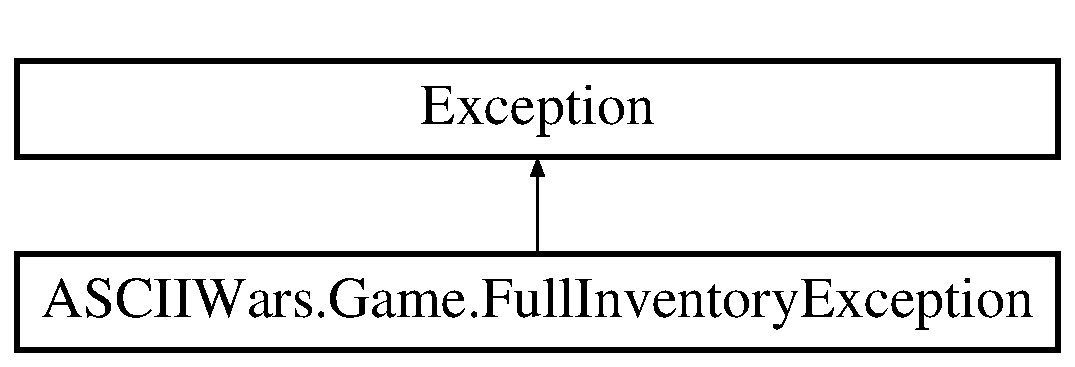
\includegraphics[height=2.000000cm]{class_a_s_c_i_i_wars_1_1_game_1_1_full_inventory_exception}
\end{center}
\end{figure}


\subsection{Подробное описание}
Исключение, которой выбрачывается при 

Объявления и описания членов класса находятся в файле\+:\begin{DoxyCompactItemize}
\item 
A\+S\+C\+I\+I\+Wars/\+Game/Player.\+cs\end{DoxyCompactItemize}

\hypertarget{class_a_s_c_i_i_wars_1_1_game_1_1_game_controller}{}\section{Класс A\+S\+C\+I\+I\+Wars.\+Game.\+Game\+Controller}
\label{class_a_s_c_i_i_wars_1_1_game_1_1_game_controller}\index{A\+S\+C\+I\+I\+Wars.\+Game.\+Game\+Controller@{A\+S\+C\+I\+I\+Wars.\+Game.\+Game\+Controller}}
\subsection*{Открытые члены}
\begin{DoxyCompactItemize}
\item 
\hyperlink{class_a_s_c_i_i_wars_1_1_game_1_1_game_controller_a9a4ad508f104af513b81824b784b0bb0}{Game\+Controller} (\hyperlink{class_a_s_c_i_i_wars_1_1_game_1_1_situation_container}{Situation\+Container} \hyperlink{class_a_s_c_i_i_wars_1_1_game_1_1_game_controller_aaab40310e11bd03711896ec5685ebe10}{situations}, \hyperlink{class_a_s_c_i_i_wars_1_1_game_1_1_item_container}{Item\+Container} \hyperlink{class_a_s_c_i_i_wars_1_1_game_1_1_game_controller_a96ab06ced4cf725ad1a4200425a533eb}{items})
\item 
void \hyperlink{class_a_s_c_i_i_wars_1_1_game_1_1_game_controller_a6a70e650d0140338ebd053c56cd55496}{Start} ()
\end{DoxyCompactItemize}
\subsection*{Открытые атрибуты}
\begin{DoxyCompactItemize}
\item 
\hyperlink{class_a_s_c_i_i_wars_1_1_game_1_1_situation_container}{Situation\+Container} \hyperlink{class_a_s_c_i_i_wars_1_1_game_1_1_game_controller_aaab40310e11bd03711896ec5685ebe10}{situations}
\item 
\hyperlink{class_a_s_c_i_i_wars_1_1_game_1_1_item_container}{Item\+Container} \hyperlink{class_a_s_c_i_i_wars_1_1_game_1_1_game_controller_a96ab06ced4cf725ad1a4200425a533eb}{items}
\item 
\hyperlink{class_a_s_c_i_i_wars_1_1_game_1_1_player}{Player} \hyperlink{class_a_s_c_i_i_wars_1_1_game_1_1_game_controller_a16a24596b98a17361e430d984f85a7ca}{player} = new \hyperlink{class_a_s_c_i_i_wars_1_1_game_1_1_player}{Player}()
\end{DoxyCompactItemize}
\subsection*{Закрытые данные}
\begin{DoxyCompactItemize}
\item 
const string \hyperlink{class_a_s_c_i_i_wars_1_1_game_1_1_game_controller_a14c3ad1eaf01d8c03789d8cc1fd09dde}{M\+A\+I\+N\+\_\+\+S\+I\+T\+U\+A\+T\+I\+O\+N\+\_\+\+N\+A\+ME} = \char`\"{}on\+Enter\char`\"{}
\item 
\hyperlink{class_a_s_c_i_i_wars_1_1_game_1_1_situation}{Situation} \hyperlink{class_a_s_c_i_i_wars_1_1_game_1_1_game_controller_ac62620afe49df42fd9f835da53e11a8b}{current\+Situation}
\end{DoxyCompactItemize}


\subsection{Конструктор(ы)}
\hypertarget{class_a_s_c_i_i_wars_1_1_game_1_1_game_controller_a9a4ad508f104af513b81824b784b0bb0}{}\label{class_a_s_c_i_i_wars_1_1_game_1_1_game_controller_a9a4ad508f104af513b81824b784b0bb0} 
\index{A\+S\+C\+I\+I\+Wars\+::\+Game\+::\+Game\+Controller@{A\+S\+C\+I\+I\+Wars\+::\+Game\+::\+Game\+Controller}!Game\+Controller@{Game\+Controller}}
\index{Game\+Controller@{Game\+Controller}!A\+S\+C\+I\+I\+Wars\+::\+Game\+::\+Game\+Controller@{A\+S\+C\+I\+I\+Wars\+::\+Game\+::\+Game\+Controller}}
\subsubsection{\texorpdfstring{Game\+Controller()}{GameController()}}
{\footnotesize\ttfamily A\+S\+C\+I\+I\+Wars.\+Game.\+Game\+Controller.\+Game\+Controller (\begin{DoxyParamCaption}\item[{\hyperlink{class_a_s_c_i_i_wars_1_1_game_1_1_situation_container}{Situation\+Container}}]{situations,  }\item[{\hyperlink{class_a_s_c_i_i_wars_1_1_game_1_1_item_container}{Item\+Container}}]{items }\end{DoxyParamCaption})\hspace{0.3cm}{\ttfamily [inline]}}



\subsection{Методы}
\hypertarget{class_a_s_c_i_i_wars_1_1_game_1_1_game_controller_a6a70e650d0140338ebd053c56cd55496}{}\label{class_a_s_c_i_i_wars_1_1_game_1_1_game_controller_a6a70e650d0140338ebd053c56cd55496} 
\index{A\+S\+C\+I\+I\+Wars\+::\+Game\+::\+Game\+Controller@{A\+S\+C\+I\+I\+Wars\+::\+Game\+::\+Game\+Controller}!Start@{Start}}
\index{Start@{Start}!A\+S\+C\+I\+I\+Wars\+::\+Game\+::\+Game\+Controller@{A\+S\+C\+I\+I\+Wars\+::\+Game\+::\+Game\+Controller}}
\subsubsection{\texorpdfstring{Start()}{Start()}}
{\footnotesize\ttfamily void A\+S\+C\+I\+I\+Wars.\+Game.\+Game\+Controller.\+Start (\begin{DoxyParamCaption}{ }\end{DoxyParamCaption})\hspace{0.3cm}{\ttfamily [inline]}}



\subsection{Данные класса}
\hypertarget{class_a_s_c_i_i_wars_1_1_game_1_1_game_controller_ac62620afe49df42fd9f835da53e11a8b}{}\label{class_a_s_c_i_i_wars_1_1_game_1_1_game_controller_ac62620afe49df42fd9f835da53e11a8b} 
\index{A\+S\+C\+I\+I\+Wars\+::\+Game\+::\+Game\+Controller@{A\+S\+C\+I\+I\+Wars\+::\+Game\+::\+Game\+Controller}!current\+Situation@{current\+Situation}}
\index{current\+Situation@{current\+Situation}!A\+S\+C\+I\+I\+Wars\+::\+Game\+::\+Game\+Controller@{A\+S\+C\+I\+I\+Wars\+::\+Game\+::\+Game\+Controller}}
\subsubsection{\texorpdfstring{current\+Situation}{currentSituation}}
{\footnotesize\ttfamily \hyperlink{class_a_s_c_i_i_wars_1_1_game_1_1_situation}{Situation} A\+S\+C\+I\+I\+Wars.\+Game.\+Game\+Controller.\+current\+Situation\hspace{0.3cm}{\ttfamily [private]}}

\hypertarget{class_a_s_c_i_i_wars_1_1_game_1_1_game_controller_a96ab06ced4cf725ad1a4200425a533eb}{}\label{class_a_s_c_i_i_wars_1_1_game_1_1_game_controller_a96ab06ced4cf725ad1a4200425a533eb} 
\index{A\+S\+C\+I\+I\+Wars\+::\+Game\+::\+Game\+Controller@{A\+S\+C\+I\+I\+Wars\+::\+Game\+::\+Game\+Controller}!items@{items}}
\index{items@{items}!A\+S\+C\+I\+I\+Wars\+::\+Game\+::\+Game\+Controller@{A\+S\+C\+I\+I\+Wars\+::\+Game\+::\+Game\+Controller}}
\subsubsection{\texorpdfstring{items}{items}}
{\footnotesize\ttfamily \hyperlink{class_a_s_c_i_i_wars_1_1_game_1_1_item_container}{Item\+Container} A\+S\+C\+I\+I\+Wars.\+Game.\+Game\+Controller.\+items}

\hypertarget{class_a_s_c_i_i_wars_1_1_game_1_1_game_controller_a14c3ad1eaf01d8c03789d8cc1fd09dde}{}\label{class_a_s_c_i_i_wars_1_1_game_1_1_game_controller_a14c3ad1eaf01d8c03789d8cc1fd09dde} 
\index{A\+S\+C\+I\+I\+Wars\+::\+Game\+::\+Game\+Controller@{A\+S\+C\+I\+I\+Wars\+::\+Game\+::\+Game\+Controller}!M\+A\+I\+N\+\_\+\+S\+I\+T\+U\+A\+T\+I\+O\+N\+\_\+\+N\+A\+ME@{M\+A\+I\+N\+\_\+\+S\+I\+T\+U\+A\+T\+I\+O\+N\+\_\+\+N\+A\+ME}}
\index{M\+A\+I\+N\+\_\+\+S\+I\+T\+U\+A\+T\+I\+O\+N\+\_\+\+N\+A\+ME@{M\+A\+I\+N\+\_\+\+S\+I\+T\+U\+A\+T\+I\+O\+N\+\_\+\+N\+A\+ME}!A\+S\+C\+I\+I\+Wars\+::\+Game\+::\+Game\+Controller@{A\+S\+C\+I\+I\+Wars\+::\+Game\+::\+Game\+Controller}}
\subsubsection{\texorpdfstring{M\+A\+I\+N\+\_\+\+S\+I\+T\+U\+A\+T\+I\+O\+N\+\_\+\+N\+A\+ME}{MAIN\_SITUATION\_NAME}}
{\footnotesize\ttfamily const string A\+S\+C\+I\+I\+Wars.\+Game.\+Game\+Controller.\+M\+A\+I\+N\+\_\+\+S\+I\+T\+U\+A\+T\+I\+O\+N\+\_\+\+N\+A\+ME = \char`\"{}on\+Enter\char`\"{}\hspace{0.3cm}{\ttfamily [private]}}

\hypertarget{class_a_s_c_i_i_wars_1_1_game_1_1_game_controller_a16a24596b98a17361e430d984f85a7ca}{}\label{class_a_s_c_i_i_wars_1_1_game_1_1_game_controller_a16a24596b98a17361e430d984f85a7ca} 
\index{A\+S\+C\+I\+I\+Wars\+::\+Game\+::\+Game\+Controller@{A\+S\+C\+I\+I\+Wars\+::\+Game\+::\+Game\+Controller}!player@{player}}
\index{player@{player}!A\+S\+C\+I\+I\+Wars\+::\+Game\+::\+Game\+Controller@{A\+S\+C\+I\+I\+Wars\+::\+Game\+::\+Game\+Controller}}
\subsubsection{\texorpdfstring{player}{player}}
{\footnotesize\ttfamily \hyperlink{class_a_s_c_i_i_wars_1_1_game_1_1_player}{Player} A\+S\+C\+I\+I\+Wars.\+Game.\+Game\+Controller.\+player = new \hyperlink{class_a_s_c_i_i_wars_1_1_game_1_1_player}{Player}()}

\hypertarget{class_a_s_c_i_i_wars_1_1_game_1_1_game_controller_aaab40310e11bd03711896ec5685ebe10}{}\label{class_a_s_c_i_i_wars_1_1_game_1_1_game_controller_aaab40310e11bd03711896ec5685ebe10} 
\index{A\+S\+C\+I\+I\+Wars\+::\+Game\+::\+Game\+Controller@{A\+S\+C\+I\+I\+Wars\+::\+Game\+::\+Game\+Controller}!situations@{situations}}
\index{situations@{situations}!A\+S\+C\+I\+I\+Wars\+::\+Game\+::\+Game\+Controller@{A\+S\+C\+I\+I\+Wars\+::\+Game\+::\+Game\+Controller}}
\subsubsection{\texorpdfstring{situations}{situations}}
{\footnotesize\ttfamily \hyperlink{class_a_s_c_i_i_wars_1_1_game_1_1_situation_container}{Situation\+Container} A\+S\+C\+I\+I\+Wars.\+Game.\+Game\+Controller.\+situations}



Объявления и описания членов класса находятся в файле\+:\begin{DoxyCompactItemize}
\item 
Game/\hyperlink{_game_controller_8cs}{Game\+Controller.\+cs}\end{DoxyCompactItemize}

\hypertarget{class_a_s_c_i_i_wars_1_1_game_1_1_health_booster}{}\section{Класс A\+S\+C\+I\+I\+Wars.\+Game.\+Health\+Booster}
\label{class_a_s_c_i_i_wars_1_1_game_1_1_health_booster}\index{A\+S\+C\+I\+I\+Wars.\+Game.\+Health\+Booster@{A\+S\+C\+I\+I\+Wars.\+Game.\+Health\+Booster}}
Граф наследования\+:A\+S\+C\+I\+I\+Wars.\+Game.\+Health\+Booster\+:\begin{figure}[H]
\begin{center}
\leavevmode
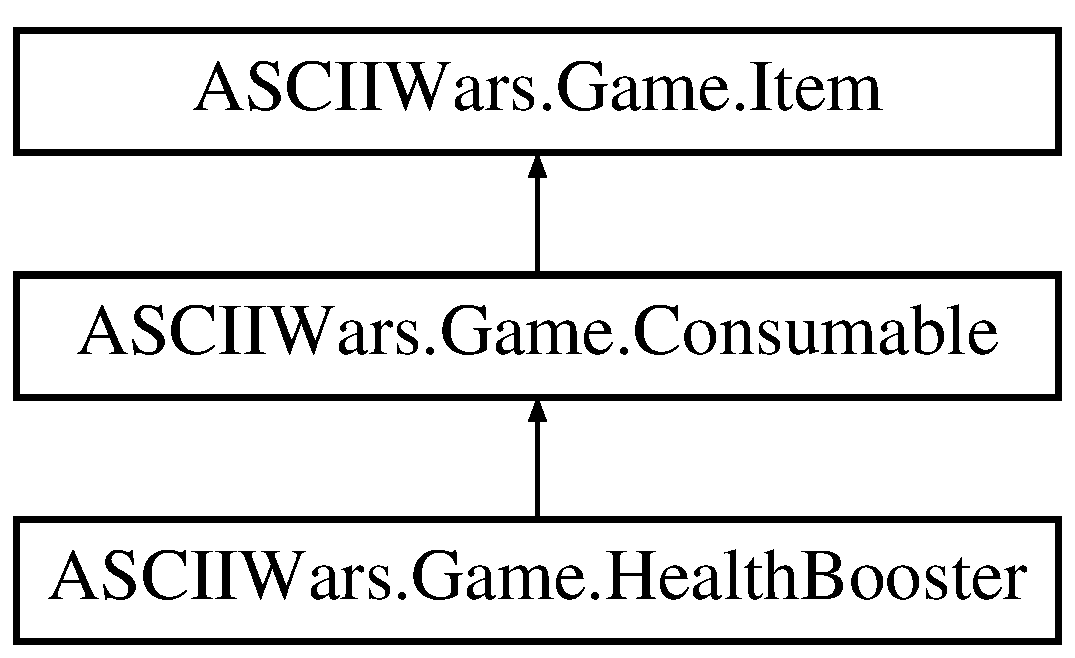
\includegraphics[height=3.000000cm]{class_a_s_c_i_i_wars_1_1_game_1_1_health_booster}
\end{center}
\end{figure}
\subsection*{Открытые члены}
\begin{DoxyCompactItemize}
\item 
\hypertarget{class_a_s_c_i_i_wars_1_1_game_1_1_health_booster_ac7796979395fc12db8b4a8d9a9ba7d7e}{}\label{class_a_s_c_i_i_wars_1_1_game_1_1_health_booster_ac7796979395fc12db8b4a8d9a9ba7d7e} 
{\bfseries Health\+Booster} (string id, string name, int health\+Boost)
\item 
\hypertarget{class_a_s_c_i_i_wars_1_1_game_1_1_health_booster_a99740fd21f80211f6a2058737b159425}{}\label{class_a_s_c_i_i_wars_1_1_game_1_1_health_booster_a99740fd21f80211f6a2058737b159425} 
override void \hyperlink{class_a_s_c_i_i_wars_1_1_game_1_1_health_booster_a99740fd21f80211f6a2058737b159425}{On\+Add\+To\+Player\+Inventory} (\hyperlink{class_a_s_c_i_i_wars_1_1_game_1_1_player}{Player} player)
\begin{DoxyCompactList}\small\item\em abc \end{DoxyCompactList}\item 
\hypertarget{class_a_s_c_i_i_wars_1_1_game_1_1_health_booster_a0dd6134e102b2b4ea9d143b7cea15568}{}\label{class_a_s_c_i_i_wars_1_1_game_1_1_health_booster_a0dd6134e102b2b4ea9d143b7cea15568} 
override void {\bfseries On\+Consume\+By\+Player} (\hyperlink{class_a_s_c_i_i_wars_1_1_game_1_1_player}{Player} player)
\item 
\hypertarget{class_a_s_c_i_i_wars_1_1_game_1_1_health_booster_ae06407b04a0e81da31c14c546d6aaaaf}{}\label{class_a_s_c_i_i_wars_1_1_game_1_1_health_booster_ae06407b04a0e81da31c14c546d6aaaaf} 
override void {\bfseries On\+Remove\+From\+Player\+Inventory} (\hyperlink{class_a_s_c_i_i_wars_1_1_game_1_1_player}{Player} player)
\item 
\hypertarget{class_a_s_c_i_i_wars_1_1_game_1_1_health_booster_a79fdb10389338ad400f723a76ce30d7d}{}\label{class_a_s_c_i_i_wars_1_1_game_1_1_health_booster_a79fdb10389338ad400f723a76ce30d7d} 
override int {\bfseries Get\+Hash\+Code} ()
\item 
\hypertarget{class_a_s_c_i_i_wars_1_1_game_1_1_health_booster_a5396e7ebb46c32e36fefeb86ab4727d3}{}\label{class_a_s_c_i_i_wars_1_1_game_1_1_health_booster_a5396e7ebb46c32e36fefeb86ab4727d3} 
override bool {\bfseries Equals} (object obj)
\end{DoxyCompactItemize}
\subsection*{Открытые атрибуты}
\begin{DoxyCompactItemize}
\item 
\hypertarget{class_a_s_c_i_i_wars_1_1_game_1_1_health_booster_abd6f83cc8e561198c5939ba4a20fd826}{}\label{class_a_s_c_i_i_wars_1_1_game_1_1_health_booster_abd6f83cc8e561198c5939ba4a20fd826} 
readonly int {\bfseries health\+Boost}
\end{DoxyCompactItemize}


Объявления и описания членов класса находятся в файле\+:\begin{DoxyCompactItemize}
\item 
A\+S\+C\+I\+I\+Wars/\+Game/Player.\+cs\end{DoxyCompactItemize}

\hypertarget{class_a_s_c_i_i_wars_1_1_game_1_1_health_potion}{}\section{Класс A\+S\+C\+I\+I\+Wars.\+Game.\+Health\+Potion}
\label{class_a_s_c_i_i_wars_1_1_game_1_1_health_potion}\index{A\+S\+C\+I\+I\+Wars.\+Game.\+Health\+Potion@{A\+S\+C\+I\+I\+Wars.\+Game.\+Health\+Potion}}
Граф наследования\+:A\+S\+C\+I\+I\+Wars.\+Game.\+Health\+Potion\+:\begin{figure}[H]
\begin{center}
\leavevmode
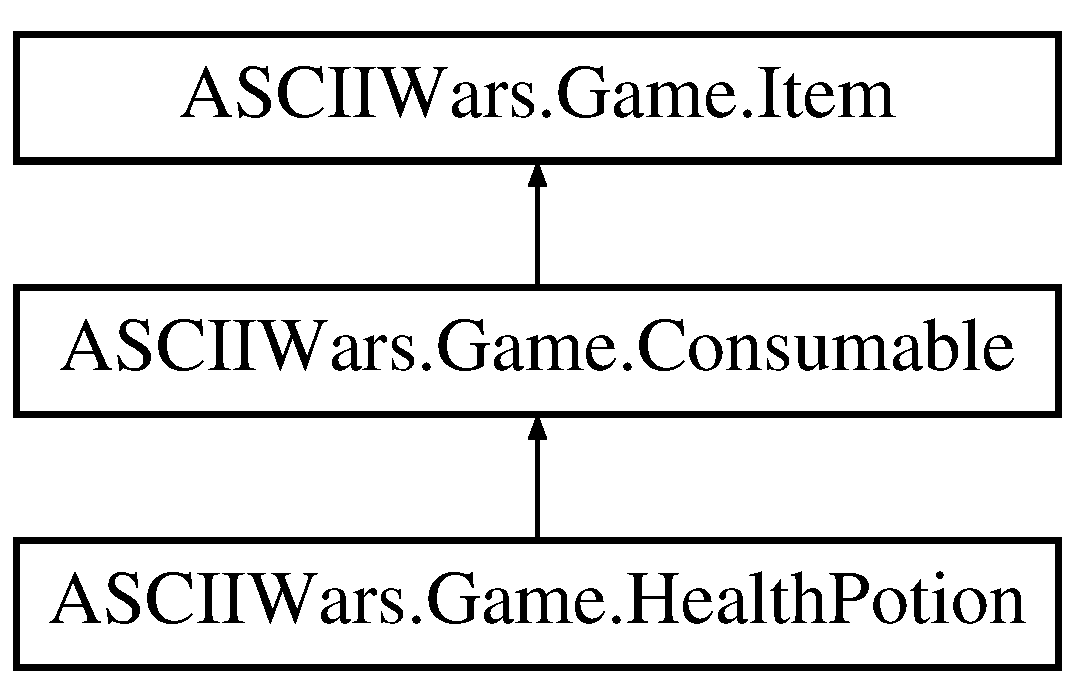
\includegraphics[height=3.000000cm]{class_a_s_c_i_i_wars_1_1_game_1_1_health_potion}
\end{center}
\end{figure}
\subsection*{Открытые члены}
\begin{DoxyCompactItemize}
\item 
\hyperlink{class_a_s_c_i_i_wars_1_1_game_1_1_health_potion_a8f1763067ff0af22657b7447fe96cc66}{Health\+Potion} (string \hyperlink{class_a_s_c_i_i_wars_1_1_game_1_1_item_a744d51f7684a4e46a1f834f8666db58e}{id}, string \hyperlink{class_a_s_c_i_i_wars_1_1_game_1_1_item_a994b9ec5f10c123e4345da159c090091}{name}, int \hyperlink{class_a_s_c_i_i_wars_1_1_game_1_1_health_potion_aa337067f250678b0825d86fc3e2868c5}{health\+Restorage})
\item 
override void \hyperlink{class_a_s_c_i_i_wars_1_1_game_1_1_health_potion_aecf685e26442760c13e59f294ce7a5e7}{On\+Add\+To\+Player\+Inventory} (\hyperlink{class_a_s_c_i_i_wars_1_1_game_1_1_player}{Player} player)
\item 
override void \hyperlink{class_a_s_c_i_i_wars_1_1_game_1_1_health_potion_a3004d1c2396e9c068ed4e03884afd56c}{On\+Consume\+By\+Player} (\hyperlink{class_a_s_c_i_i_wars_1_1_game_1_1_player}{Player} player)
\item 
override void \hyperlink{class_a_s_c_i_i_wars_1_1_game_1_1_health_potion_ad708f58b7d3cbc69945cb2ccb0328f78}{On\+Remove\+From\+Player\+Inventory} (\hyperlink{class_a_s_c_i_i_wars_1_1_game_1_1_player}{Player} player)
\item 
override int \hyperlink{class_a_s_c_i_i_wars_1_1_game_1_1_health_potion_a825fcf689ad6dd4fcf48069980f8c176}{Get\+Hash\+Code} ()
\item 
override bool \hyperlink{class_a_s_c_i_i_wars_1_1_game_1_1_health_potion_a84ed6d197746ebb5a33a61b2b2e46fb9}{Equals} (object obj)
\end{DoxyCompactItemize}
\subsection*{Открытые атрибуты}
\begin{DoxyCompactItemize}
\item 
readonly int \hyperlink{class_a_s_c_i_i_wars_1_1_game_1_1_health_potion_aa337067f250678b0825d86fc3e2868c5}{health\+Restorage}
\end{DoxyCompactItemize}


\subsection{Конструктор(ы)}
\hypertarget{class_a_s_c_i_i_wars_1_1_game_1_1_health_potion_a8f1763067ff0af22657b7447fe96cc66}{}\label{class_a_s_c_i_i_wars_1_1_game_1_1_health_potion_a8f1763067ff0af22657b7447fe96cc66} 
\index{A\+S\+C\+I\+I\+Wars\+::\+Game\+::\+Health\+Potion@{A\+S\+C\+I\+I\+Wars\+::\+Game\+::\+Health\+Potion}!Health\+Potion@{Health\+Potion}}
\index{Health\+Potion@{Health\+Potion}!A\+S\+C\+I\+I\+Wars\+::\+Game\+::\+Health\+Potion@{A\+S\+C\+I\+I\+Wars\+::\+Game\+::\+Health\+Potion}}
\subsubsection{\texorpdfstring{Health\+Potion()}{HealthPotion()}}
{\footnotesize\ttfamily A\+S\+C\+I\+I\+Wars.\+Game.\+Health\+Potion.\+Health\+Potion (\begin{DoxyParamCaption}\item[{string}]{id,  }\item[{string}]{name,  }\item[{int}]{health\+Restorage }\end{DoxyParamCaption})\hspace{0.3cm}{\ttfamily [inline]}}



\subsection{Методы}
\hypertarget{class_a_s_c_i_i_wars_1_1_game_1_1_health_potion_a84ed6d197746ebb5a33a61b2b2e46fb9}{}\label{class_a_s_c_i_i_wars_1_1_game_1_1_health_potion_a84ed6d197746ebb5a33a61b2b2e46fb9} 
\index{A\+S\+C\+I\+I\+Wars\+::\+Game\+::\+Health\+Potion@{A\+S\+C\+I\+I\+Wars\+::\+Game\+::\+Health\+Potion}!Equals@{Equals}}
\index{Equals@{Equals}!A\+S\+C\+I\+I\+Wars\+::\+Game\+::\+Health\+Potion@{A\+S\+C\+I\+I\+Wars\+::\+Game\+::\+Health\+Potion}}
\subsubsection{\texorpdfstring{Equals()}{Equals()}}
{\footnotesize\ttfamily override bool A\+S\+C\+I\+I\+Wars.\+Game.\+Health\+Potion.\+Equals (\begin{DoxyParamCaption}\item[{object}]{obj }\end{DoxyParamCaption})\hspace{0.3cm}{\ttfamily [inline]}}

\hypertarget{class_a_s_c_i_i_wars_1_1_game_1_1_health_potion_a825fcf689ad6dd4fcf48069980f8c176}{}\label{class_a_s_c_i_i_wars_1_1_game_1_1_health_potion_a825fcf689ad6dd4fcf48069980f8c176} 
\index{A\+S\+C\+I\+I\+Wars\+::\+Game\+::\+Health\+Potion@{A\+S\+C\+I\+I\+Wars\+::\+Game\+::\+Health\+Potion}!Get\+Hash\+Code@{Get\+Hash\+Code}}
\index{Get\+Hash\+Code@{Get\+Hash\+Code}!A\+S\+C\+I\+I\+Wars\+::\+Game\+::\+Health\+Potion@{A\+S\+C\+I\+I\+Wars\+::\+Game\+::\+Health\+Potion}}
\subsubsection{\texorpdfstring{Get\+Hash\+Code()}{GetHashCode()}}
{\footnotesize\ttfamily override int A\+S\+C\+I\+I\+Wars.\+Game.\+Health\+Potion.\+Get\+Hash\+Code (\begin{DoxyParamCaption}{ }\end{DoxyParamCaption})\hspace{0.3cm}{\ttfamily [inline]}}

\hypertarget{class_a_s_c_i_i_wars_1_1_game_1_1_health_potion_aecf685e26442760c13e59f294ce7a5e7}{}\label{class_a_s_c_i_i_wars_1_1_game_1_1_health_potion_aecf685e26442760c13e59f294ce7a5e7} 
\index{A\+S\+C\+I\+I\+Wars\+::\+Game\+::\+Health\+Potion@{A\+S\+C\+I\+I\+Wars\+::\+Game\+::\+Health\+Potion}!On\+Add\+To\+Player\+Inventory@{On\+Add\+To\+Player\+Inventory}}
\index{On\+Add\+To\+Player\+Inventory@{On\+Add\+To\+Player\+Inventory}!A\+S\+C\+I\+I\+Wars\+::\+Game\+::\+Health\+Potion@{A\+S\+C\+I\+I\+Wars\+::\+Game\+::\+Health\+Potion}}
\subsubsection{\texorpdfstring{On\+Add\+To\+Player\+Inventory()}{OnAddToPlayerInventory()}}
{\footnotesize\ttfamily override void A\+S\+C\+I\+I\+Wars.\+Game.\+Health\+Potion.\+On\+Add\+To\+Player\+Inventory (\begin{DoxyParamCaption}\item[{\hyperlink{class_a_s_c_i_i_wars_1_1_game_1_1_player}{Player}}]{player }\end{DoxyParamCaption})\hspace{0.3cm}{\ttfamily [inline]}, {\ttfamily [virtual]}}



Замещает \hyperlink{class_a_s_c_i_i_wars_1_1_game_1_1_item_aec0355b7a9f647ef24897b95563f70d1}{A\+S\+C\+I\+I\+Wars.\+Game.\+Item}.

\hypertarget{class_a_s_c_i_i_wars_1_1_game_1_1_health_potion_a3004d1c2396e9c068ed4e03884afd56c}{}\label{class_a_s_c_i_i_wars_1_1_game_1_1_health_potion_a3004d1c2396e9c068ed4e03884afd56c} 
\index{A\+S\+C\+I\+I\+Wars\+::\+Game\+::\+Health\+Potion@{A\+S\+C\+I\+I\+Wars\+::\+Game\+::\+Health\+Potion}!On\+Consume\+By\+Player@{On\+Consume\+By\+Player}}
\index{On\+Consume\+By\+Player@{On\+Consume\+By\+Player}!A\+S\+C\+I\+I\+Wars\+::\+Game\+::\+Health\+Potion@{A\+S\+C\+I\+I\+Wars\+::\+Game\+::\+Health\+Potion}}
\subsubsection{\texorpdfstring{On\+Consume\+By\+Player()}{OnConsumeByPlayer()}}
{\footnotesize\ttfamily override void A\+S\+C\+I\+I\+Wars.\+Game.\+Health\+Potion.\+On\+Consume\+By\+Player (\begin{DoxyParamCaption}\item[{\hyperlink{class_a_s_c_i_i_wars_1_1_game_1_1_player}{Player}}]{player }\end{DoxyParamCaption})\hspace{0.3cm}{\ttfamily [inline]}, {\ttfamily [virtual]}}



Замещает \hyperlink{class_a_s_c_i_i_wars_1_1_game_1_1_consumable_a6aac67fe076ca39cb850e3720461fff8}{A\+S\+C\+I\+I\+Wars.\+Game.\+Consumable}.

\hypertarget{class_a_s_c_i_i_wars_1_1_game_1_1_health_potion_ad708f58b7d3cbc69945cb2ccb0328f78}{}\label{class_a_s_c_i_i_wars_1_1_game_1_1_health_potion_ad708f58b7d3cbc69945cb2ccb0328f78} 
\index{A\+S\+C\+I\+I\+Wars\+::\+Game\+::\+Health\+Potion@{A\+S\+C\+I\+I\+Wars\+::\+Game\+::\+Health\+Potion}!On\+Remove\+From\+Player\+Inventory@{On\+Remove\+From\+Player\+Inventory}}
\index{On\+Remove\+From\+Player\+Inventory@{On\+Remove\+From\+Player\+Inventory}!A\+S\+C\+I\+I\+Wars\+::\+Game\+::\+Health\+Potion@{A\+S\+C\+I\+I\+Wars\+::\+Game\+::\+Health\+Potion}}
\subsubsection{\texorpdfstring{On\+Remove\+From\+Player\+Inventory()}{OnRemoveFromPlayerInventory()}}
{\footnotesize\ttfamily override void A\+S\+C\+I\+I\+Wars.\+Game.\+Health\+Potion.\+On\+Remove\+From\+Player\+Inventory (\begin{DoxyParamCaption}\item[{\hyperlink{class_a_s_c_i_i_wars_1_1_game_1_1_player}{Player}}]{player }\end{DoxyParamCaption})\hspace{0.3cm}{\ttfamily [inline]}, {\ttfamily [virtual]}}



Замещает \hyperlink{class_a_s_c_i_i_wars_1_1_game_1_1_item_a52412546f837bfc65a3aa9d728fa142f}{A\+S\+C\+I\+I\+Wars.\+Game.\+Item}.



\subsection{Данные класса}
\hypertarget{class_a_s_c_i_i_wars_1_1_game_1_1_health_potion_aa337067f250678b0825d86fc3e2868c5}{}\label{class_a_s_c_i_i_wars_1_1_game_1_1_health_potion_aa337067f250678b0825d86fc3e2868c5} 
\index{A\+S\+C\+I\+I\+Wars\+::\+Game\+::\+Health\+Potion@{A\+S\+C\+I\+I\+Wars\+::\+Game\+::\+Health\+Potion}!health\+Restorage@{health\+Restorage}}
\index{health\+Restorage@{health\+Restorage}!A\+S\+C\+I\+I\+Wars\+::\+Game\+::\+Health\+Potion@{A\+S\+C\+I\+I\+Wars\+::\+Game\+::\+Health\+Potion}}
\subsubsection{\texorpdfstring{health\+Restorage}{healthRestorage}}
{\footnotesize\ttfamily readonly int A\+S\+C\+I\+I\+Wars.\+Game.\+Health\+Potion.\+health\+Restorage}



Объявления и описания членов класса находятся в файле\+:\begin{DoxyCompactItemize}
\item 
Game/\hyperlink{_player_8cs}{Player.\+cs}\end{DoxyCompactItemize}

\hypertarget{class_a_s_c_i_i_wars_1_1_game_1_1_item}{}\section{Класс A\+S\+C\+I\+I\+Wars.\+Game.\+Item}
\label{class_a_s_c_i_i_wars_1_1_game_1_1_item}\index{A\+S\+C\+I\+I\+Wars.\+Game.\+Item@{A\+S\+C\+I\+I\+Wars.\+Game.\+Item}}
Граф наследования\+:A\+S\+C\+I\+I\+Wars.\+Game.\+Item\+:\begin{figure}[H]
\begin{center}
\leavevmode
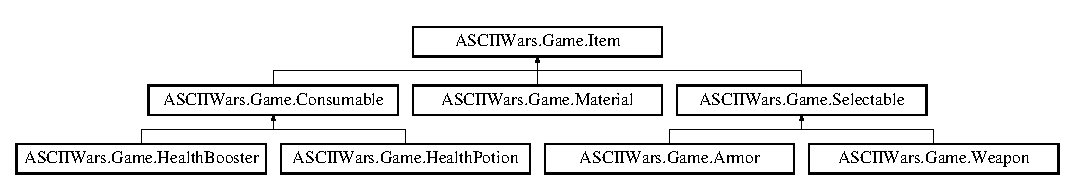
\includegraphics[height=2.100000cm]{class_a_s_c_i_i_wars_1_1_game_1_1_item}
\end{center}
\end{figure}
\subsection*{Открытые члены}
\begin{DoxyCompactItemize}
\item 
\hyperlink{class_a_s_c_i_i_wars_1_1_game_1_1_item_ae9b7ebce1c577c6d4e142f7d8f736ec5}{Item} (string \hyperlink{class_a_s_c_i_i_wars_1_1_game_1_1_item_a744d51f7684a4e46a1f834f8666db58e}{id}, string \hyperlink{class_a_s_c_i_i_wars_1_1_game_1_1_item_a994b9ec5f10c123e4345da159c090091}{name}, string \hyperlink{class_a_s_c_i_i_wars_1_1_game_1_1_item_a6ff41e953ccebc64a8df8f8c434535a0}{description})
\item 
abstract void \hyperlink{class_a_s_c_i_i_wars_1_1_game_1_1_item_aec0355b7a9f647ef24897b95563f70d1}{On\+Add\+To\+Player\+Inventory} (\hyperlink{class_a_s_c_i_i_wars_1_1_game_1_1_player}{Player} player)
\item 
abstract void \hyperlink{class_a_s_c_i_i_wars_1_1_game_1_1_item_a52412546f837bfc65a3aa9d728fa142f}{On\+Remove\+From\+Player\+Inventory} (\hyperlink{class_a_s_c_i_i_wars_1_1_game_1_1_player}{Player} player)
\item 
override int \hyperlink{class_a_s_c_i_i_wars_1_1_game_1_1_item_aa503cb0e59f19deb5124271048735de4}{Get\+Hash\+Code} ()
\item 
override bool \hyperlink{class_a_s_c_i_i_wars_1_1_game_1_1_item_a8a91f74db078fbb15657f28ef92155f8}{Equals} (object obj)
\end{DoxyCompactItemize}
\subsection*{Открытые атрибуты}
\begin{DoxyCompactItemize}
\item 
readonly string \hyperlink{class_a_s_c_i_i_wars_1_1_game_1_1_item_a744d51f7684a4e46a1f834f8666db58e}{id}
\item 
readonly string \hyperlink{class_a_s_c_i_i_wars_1_1_game_1_1_item_a994b9ec5f10c123e4345da159c090091}{name}
\item 
readonly string \hyperlink{class_a_s_c_i_i_wars_1_1_game_1_1_item_a6ff41e953ccebc64a8df8f8c434535a0}{description}
\end{DoxyCompactItemize}


\subsection{Конструктор(ы)}
\hypertarget{class_a_s_c_i_i_wars_1_1_game_1_1_item_ae9b7ebce1c577c6d4e142f7d8f736ec5}{}\label{class_a_s_c_i_i_wars_1_1_game_1_1_item_ae9b7ebce1c577c6d4e142f7d8f736ec5} 
\index{A\+S\+C\+I\+I\+Wars\+::\+Game\+::\+Item@{A\+S\+C\+I\+I\+Wars\+::\+Game\+::\+Item}!Item@{Item}}
\index{Item@{Item}!A\+S\+C\+I\+I\+Wars\+::\+Game\+::\+Item@{A\+S\+C\+I\+I\+Wars\+::\+Game\+::\+Item}}
\subsubsection{\texorpdfstring{Item()}{Item()}}
{\footnotesize\ttfamily A\+S\+C\+I\+I\+Wars.\+Game.\+Item.\+Item (\begin{DoxyParamCaption}\item[{string}]{id,  }\item[{string}]{name,  }\item[{string}]{description }\end{DoxyParamCaption})\hspace{0.3cm}{\ttfamily [inline]}}



\subsection{Методы}
\hypertarget{class_a_s_c_i_i_wars_1_1_game_1_1_item_a8a91f74db078fbb15657f28ef92155f8}{}\label{class_a_s_c_i_i_wars_1_1_game_1_1_item_a8a91f74db078fbb15657f28ef92155f8} 
\index{A\+S\+C\+I\+I\+Wars\+::\+Game\+::\+Item@{A\+S\+C\+I\+I\+Wars\+::\+Game\+::\+Item}!Equals@{Equals}}
\index{Equals@{Equals}!A\+S\+C\+I\+I\+Wars\+::\+Game\+::\+Item@{A\+S\+C\+I\+I\+Wars\+::\+Game\+::\+Item}}
\subsubsection{\texorpdfstring{Equals()}{Equals()}}
{\footnotesize\ttfamily override bool A\+S\+C\+I\+I\+Wars.\+Game.\+Item.\+Equals (\begin{DoxyParamCaption}\item[{object}]{obj }\end{DoxyParamCaption})\hspace{0.3cm}{\ttfamily [inline]}}

\hypertarget{class_a_s_c_i_i_wars_1_1_game_1_1_item_aa503cb0e59f19deb5124271048735de4}{}\label{class_a_s_c_i_i_wars_1_1_game_1_1_item_aa503cb0e59f19deb5124271048735de4} 
\index{A\+S\+C\+I\+I\+Wars\+::\+Game\+::\+Item@{A\+S\+C\+I\+I\+Wars\+::\+Game\+::\+Item}!Get\+Hash\+Code@{Get\+Hash\+Code}}
\index{Get\+Hash\+Code@{Get\+Hash\+Code}!A\+S\+C\+I\+I\+Wars\+::\+Game\+::\+Item@{A\+S\+C\+I\+I\+Wars\+::\+Game\+::\+Item}}
\subsubsection{\texorpdfstring{Get\+Hash\+Code()}{GetHashCode()}}
{\footnotesize\ttfamily override int A\+S\+C\+I\+I\+Wars.\+Game.\+Item.\+Get\+Hash\+Code (\begin{DoxyParamCaption}{ }\end{DoxyParamCaption})\hspace{0.3cm}{\ttfamily [inline]}}

\hypertarget{class_a_s_c_i_i_wars_1_1_game_1_1_item_aec0355b7a9f647ef24897b95563f70d1}{}\label{class_a_s_c_i_i_wars_1_1_game_1_1_item_aec0355b7a9f647ef24897b95563f70d1} 
\index{A\+S\+C\+I\+I\+Wars\+::\+Game\+::\+Item@{A\+S\+C\+I\+I\+Wars\+::\+Game\+::\+Item}!On\+Add\+To\+Player\+Inventory@{On\+Add\+To\+Player\+Inventory}}
\index{On\+Add\+To\+Player\+Inventory@{On\+Add\+To\+Player\+Inventory}!A\+S\+C\+I\+I\+Wars\+::\+Game\+::\+Item@{A\+S\+C\+I\+I\+Wars\+::\+Game\+::\+Item}}
\subsubsection{\texorpdfstring{On\+Add\+To\+Player\+Inventory()}{OnAddToPlayerInventory()}}
{\footnotesize\ttfamily abstract void A\+S\+C\+I\+I\+Wars.\+Game.\+Item.\+On\+Add\+To\+Player\+Inventory (\begin{DoxyParamCaption}\item[{\hyperlink{class_a_s_c_i_i_wars_1_1_game_1_1_player}{Player}}]{player }\end{DoxyParamCaption})\hspace{0.3cm}{\ttfamily [pure virtual]}}



Замещается в \hyperlink{class_a_s_c_i_i_wars_1_1_game_1_1_material_afedb9d9b8b22782e40371b6cac37d27e}{A\+S\+C\+I\+I\+Wars.\+Game.\+Material}, \hyperlink{class_a_s_c_i_i_wars_1_1_game_1_1_health_booster_a99740fd21f80211f6a2058737b159425}{A\+S\+C\+I\+I\+Wars.\+Game.\+Health\+Booster}, \hyperlink{class_a_s_c_i_i_wars_1_1_game_1_1_health_potion_aecf685e26442760c13e59f294ce7a5e7}{A\+S\+C\+I\+I\+Wars.\+Game.\+Health\+Potion}, \hyperlink{class_a_s_c_i_i_wars_1_1_game_1_1_armor_ab8e1364e91ddd19f7c214f051b054cd8}{A\+S\+C\+I\+I\+Wars.\+Game.\+Armor} и \hyperlink{class_a_s_c_i_i_wars_1_1_game_1_1_weapon_ad29135a3edb4ea03f29163d788364299}{A\+S\+C\+I\+I\+Wars.\+Game.\+Weapon}.

\hypertarget{class_a_s_c_i_i_wars_1_1_game_1_1_item_a52412546f837bfc65a3aa9d728fa142f}{}\label{class_a_s_c_i_i_wars_1_1_game_1_1_item_a52412546f837bfc65a3aa9d728fa142f} 
\index{A\+S\+C\+I\+I\+Wars\+::\+Game\+::\+Item@{A\+S\+C\+I\+I\+Wars\+::\+Game\+::\+Item}!On\+Remove\+From\+Player\+Inventory@{On\+Remove\+From\+Player\+Inventory}}
\index{On\+Remove\+From\+Player\+Inventory@{On\+Remove\+From\+Player\+Inventory}!A\+S\+C\+I\+I\+Wars\+::\+Game\+::\+Item@{A\+S\+C\+I\+I\+Wars\+::\+Game\+::\+Item}}
\subsubsection{\texorpdfstring{On\+Remove\+From\+Player\+Inventory()}{OnRemoveFromPlayerInventory()}}
{\footnotesize\ttfamily abstract void A\+S\+C\+I\+I\+Wars.\+Game.\+Item.\+On\+Remove\+From\+Player\+Inventory (\begin{DoxyParamCaption}\item[{\hyperlink{class_a_s_c_i_i_wars_1_1_game_1_1_player}{Player}}]{player }\end{DoxyParamCaption})\hspace{0.3cm}{\ttfamily [pure virtual]}}



Замещается в \hyperlink{class_a_s_c_i_i_wars_1_1_game_1_1_material_ab8467edc48ff6af4021f550c97cbec31}{A\+S\+C\+I\+I\+Wars.\+Game.\+Material}, \hyperlink{class_a_s_c_i_i_wars_1_1_game_1_1_health_booster_ae06407b04a0e81da31c14c546d6aaaaf}{A\+S\+C\+I\+I\+Wars.\+Game.\+Health\+Booster}, \hyperlink{class_a_s_c_i_i_wars_1_1_game_1_1_health_potion_ad708f58b7d3cbc69945cb2ccb0328f78}{A\+S\+C\+I\+I\+Wars.\+Game.\+Health\+Potion}, \hyperlink{class_a_s_c_i_i_wars_1_1_game_1_1_armor_ab113733825094b12aba14b8b48372f9c}{A\+S\+C\+I\+I\+Wars.\+Game.\+Armor} и \hyperlink{class_a_s_c_i_i_wars_1_1_game_1_1_weapon_a1fc9edec1d3881aee188a30ddc8f9e58}{A\+S\+C\+I\+I\+Wars.\+Game.\+Weapon}.



\subsection{Данные класса}
\hypertarget{class_a_s_c_i_i_wars_1_1_game_1_1_item_a6ff41e953ccebc64a8df8f8c434535a0}{}\label{class_a_s_c_i_i_wars_1_1_game_1_1_item_a6ff41e953ccebc64a8df8f8c434535a0} 
\index{A\+S\+C\+I\+I\+Wars\+::\+Game\+::\+Item@{A\+S\+C\+I\+I\+Wars\+::\+Game\+::\+Item}!description@{description}}
\index{description@{description}!A\+S\+C\+I\+I\+Wars\+::\+Game\+::\+Item@{A\+S\+C\+I\+I\+Wars\+::\+Game\+::\+Item}}
\subsubsection{\texorpdfstring{description}{description}}
{\footnotesize\ttfamily readonly string A\+S\+C\+I\+I\+Wars.\+Game.\+Item.\+description}

\hypertarget{class_a_s_c_i_i_wars_1_1_game_1_1_item_a744d51f7684a4e46a1f834f8666db58e}{}\label{class_a_s_c_i_i_wars_1_1_game_1_1_item_a744d51f7684a4e46a1f834f8666db58e} 
\index{A\+S\+C\+I\+I\+Wars\+::\+Game\+::\+Item@{A\+S\+C\+I\+I\+Wars\+::\+Game\+::\+Item}!id@{id}}
\index{id@{id}!A\+S\+C\+I\+I\+Wars\+::\+Game\+::\+Item@{A\+S\+C\+I\+I\+Wars\+::\+Game\+::\+Item}}
\subsubsection{\texorpdfstring{id}{id}}
{\footnotesize\ttfamily readonly string A\+S\+C\+I\+I\+Wars.\+Game.\+Item.\+id}

\hypertarget{class_a_s_c_i_i_wars_1_1_game_1_1_item_a994b9ec5f10c123e4345da159c090091}{}\label{class_a_s_c_i_i_wars_1_1_game_1_1_item_a994b9ec5f10c123e4345da159c090091} 
\index{A\+S\+C\+I\+I\+Wars\+::\+Game\+::\+Item@{A\+S\+C\+I\+I\+Wars\+::\+Game\+::\+Item}!name@{name}}
\index{name@{name}!A\+S\+C\+I\+I\+Wars\+::\+Game\+::\+Item@{A\+S\+C\+I\+I\+Wars\+::\+Game\+::\+Item}}
\subsubsection{\texorpdfstring{name}{name}}
{\footnotesize\ttfamily readonly string A\+S\+C\+I\+I\+Wars.\+Game.\+Item.\+name}



Объявления и описания членов класса находятся в файле\+:\begin{DoxyCompactItemize}
\item 
Game/\hyperlink{_player_8cs}{Player.\+cs}\end{DoxyCompactItemize}

\hypertarget{class_a_s_c_i_i_wars_1_1_game_1_1_item_container}{}\section{Класс A\+S\+C\+I\+I\+Wars.\+Game.\+Item\+Container}
\label{class_a_s_c_i_i_wars_1_1_game_1_1_item_container}\index{A\+S\+C\+I\+I\+Wars.\+Game.\+Item\+Container@{A\+S\+C\+I\+I\+Wars.\+Game.\+Item\+Container}}
\subsection*{Открытые члены}
\begin{DoxyCompactItemize}
\item 
\hyperlink{class_a_s_c_i_i_wars_1_1_game_1_1_armor}{Armor} \hyperlink{class_a_s_c_i_i_wars_1_1_game_1_1_item_container_a4aa8a9dc347ac6b8b24486567110c802}{Get\+Armor} (string id)
\item 
\hyperlink{class_a_s_c_i_i_wars_1_1_game_1_1_weapon}{Weapon} \hyperlink{class_a_s_c_i_i_wars_1_1_game_1_1_item_container_aae0cb532c9242a5673e80eaff7b3edbd}{Get\+Weapon} (string id)
\item 
\hyperlink{class_a_s_c_i_i_wars_1_1_game_1_1_health_potion}{Health\+Potion} \hyperlink{class_a_s_c_i_i_wars_1_1_game_1_1_item_container_a449041c4df0b261569597be88277d92b}{Get\+Health\+Potion} (string id)
\item 
\hyperlink{class_a_s_c_i_i_wars_1_1_game_1_1_health_booster}{Health\+Booster} \hyperlink{class_a_s_c_i_i_wars_1_1_game_1_1_item_container_aa70c43020c6a423188df77bd7087feb1}{Get\+Health\+Booster} (string id)
\item 
\hyperlink{class_a_s_c_i_i_wars_1_1_game_1_1_material}{Material} \hyperlink{class_a_s_c_i_i_wars_1_1_game_1_1_item_container_a75b28ef2b5ae3acfceeb787c95eeb34b}{Get\+Material} (string id)
\item 
Tuple$<$ \hyperlink{class_a_s_c_i_i_wars_1_1_game_1_1_item}{Item}, int $>$ \hyperlink{class_a_s_c_i_i_wars_1_1_game_1_1_item_container_a0767f02c52f2192deeb1ad1276ef2351}{Resolve\+Reference\+And\+Count} (\hyperlink{class_a_s_c_i_i_wars_1_1_game_1_1_item_reference}{Item\+Reference} reference)
\item 
\hyperlink{class_a_s_c_i_i_wars_1_1_game_1_1_item}{Item} \hyperlink{class_a_s_c_i_i_wars_1_1_game_1_1_item_container_a289dd8937aa0feda17c2e8df1a2779ff}{Resolve\+Reference} (\hyperlink{class_a_s_c_i_i_wars_1_1_game_1_1_item_reference}{Item\+Reference} reference)
\item 
\hyperlink{class_a_s_c_i_i_wars_1_1_game_1_1_item}{Item} \hyperlink{class_a_s_c_i_i_wars_1_1_game_1_1_item_container_aec1dfc18aa9c761e15c5421f50691331}{Get\+By\+Type\+And\+ID} (string item\+Type, string item\+ID)
\end{DoxyCompactItemize}
\subsection*{Свойства}
\begin{DoxyCompactItemize}
\item 
Dictionary$<$ string, \hyperlink{class_a_s_c_i_i_wars_1_1_game_1_1_j_s_o_n_armor}{J\+S\+O\+N\+Armor} $>$ \hyperlink{class_a_s_c_i_i_wars_1_1_game_1_1_item_container_ac7163583c5b161a5621b1d8c8eecb628}{armors}\hspace{0.3cm}{\ttfamily  \mbox{[}get, set\mbox{]}}
\item 
Dictionary$<$ string, \hyperlink{class_a_s_c_i_i_wars_1_1_game_1_1_j_s_o_n_weapon}{J\+S\+O\+N\+Weapon} $>$ \hyperlink{class_a_s_c_i_i_wars_1_1_game_1_1_item_container_aaa8cd3f87c9f17712bca4ea090166ce7}{weapons}\hspace{0.3cm}{\ttfamily  \mbox{[}get, set\mbox{]}}
\item 
Dictionary$<$ string, \hyperlink{class_a_s_c_i_i_wars_1_1_game_1_1_j_s_o_n_health_potion}{J\+S\+O\+N\+Health\+Potion} $>$ \hyperlink{class_a_s_c_i_i_wars_1_1_game_1_1_item_container_a84c795ebe8785d1d14dad75b7670f68a}{health\+Potions}\hspace{0.3cm}{\ttfamily  \mbox{[}get, set\mbox{]}}
\item 
Dictionary$<$ string, \hyperlink{class_a_s_c_i_i_wars_1_1_game_1_1_j_s_o_n_health_booster}{J\+S\+O\+N\+Health\+Booster} $>$ \hyperlink{class_a_s_c_i_i_wars_1_1_game_1_1_item_container_aaecb48567ec96981ee40734e45f3339b}{health\+Boosters}\hspace{0.3cm}{\ttfamily  \mbox{[}get, set\mbox{]}}
\item 
Dictionary$<$ string, \hyperlink{class_a_s_c_i_i_wars_1_1_game_1_1_j_s_o_n_material}{J\+S\+O\+N\+Material} $>$ \hyperlink{class_a_s_c_i_i_wars_1_1_game_1_1_item_container_a503bd6d21fce823b843969ccf07871bd}{materials}\hspace{0.3cm}{\ttfamily  \mbox{[}get, set\mbox{]}}
\end{DoxyCompactItemize}


\subsection{Методы}
\hypertarget{class_a_s_c_i_i_wars_1_1_game_1_1_item_container_a4aa8a9dc347ac6b8b24486567110c802}{}\label{class_a_s_c_i_i_wars_1_1_game_1_1_item_container_a4aa8a9dc347ac6b8b24486567110c802} 
\index{A\+S\+C\+I\+I\+Wars\+::\+Game\+::\+Item\+Container@{A\+S\+C\+I\+I\+Wars\+::\+Game\+::\+Item\+Container}!Get\+Armor@{Get\+Armor}}
\index{Get\+Armor@{Get\+Armor}!A\+S\+C\+I\+I\+Wars\+::\+Game\+::\+Item\+Container@{A\+S\+C\+I\+I\+Wars\+::\+Game\+::\+Item\+Container}}
\subsubsection{\texorpdfstring{Get\+Armor()}{GetArmor()}}
{\footnotesize\ttfamily \hyperlink{class_a_s_c_i_i_wars_1_1_game_1_1_armor}{Armor} A\+S\+C\+I\+I\+Wars.\+Game.\+Item\+Container.\+Get\+Armor (\begin{DoxyParamCaption}\item[{string}]{id }\end{DoxyParamCaption})\hspace{0.3cm}{\ttfamily [inline]}}

\hypertarget{class_a_s_c_i_i_wars_1_1_game_1_1_item_container_aec1dfc18aa9c761e15c5421f50691331}{}\label{class_a_s_c_i_i_wars_1_1_game_1_1_item_container_aec1dfc18aa9c761e15c5421f50691331} 
\index{A\+S\+C\+I\+I\+Wars\+::\+Game\+::\+Item\+Container@{A\+S\+C\+I\+I\+Wars\+::\+Game\+::\+Item\+Container}!Get\+By\+Type\+And\+ID@{Get\+By\+Type\+And\+ID}}
\index{Get\+By\+Type\+And\+ID@{Get\+By\+Type\+And\+ID}!A\+S\+C\+I\+I\+Wars\+::\+Game\+::\+Item\+Container@{A\+S\+C\+I\+I\+Wars\+::\+Game\+::\+Item\+Container}}
\subsubsection{\texorpdfstring{Get\+By\+Type\+And\+I\+D()}{GetByTypeAndID()}}
{\footnotesize\ttfamily \hyperlink{class_a_s_c_i_i_wars_1_1_game_1_1_item}{Item} A\+S\+C\+I\+I\+Wars.\+Game.\+Item\+Container.\+Get\+By\+Type\+And\+ID (\begin{DoxyParamCaption}\item[{string}]{item\+Type,  }\item[{string}]{item\+ID }\end{DoxyParamCaption})\hspace{0.3cm}{\ttfamily [inline]}}

\hypertarget{class_a_s_c_i_i_wars_1_1_game_1_1_item_container_aa70c43020c6a423188df77bd7087feb1}{}\label{class_a_s_c_i_i_wars_1_1_game_1_1_item_container_aa70c43020c6a423188df77bd7087feb1} 
\index{A\+S\+C\+I\+I\+Wars\+::\+Game\+::\+Item\+Container@{A\+S\+C\+I\+I\+Wars\+::\+Game\+::\+Item\+Container}!Get\+Health\+Booster@{Get\+Health\+Booster}}
\index{Get\+Health\+Booster@{Get\+Health\+Booster}!A\+S\+C\+I\+I\+Wars\+::\+Game\+::\+Item\+Container@{A\+S\+C\+I\+I\+Wars\+::\+Game\+::\+Item\+Container}}
\subsubsection{\texorpdfstring{Get\+Health\+Booster()}{GetHealthBooster()}}
{\footnotesize\ttfamily \hyperlink{class_a_s_c_i_i_wars_1_1_game_1_1_health_booster}{Health\+Booster} A\+S\+C\+I\+I\+Wars.\+Game.\+Item\+Container.\+Get\+Health\+Booster (\begin{DoxyParamCaption}\item[{string}]{id }\end{DoxyParamCaption})\hspace{0.3cm}{\ttfamily [inline]}}

\hypertarget{class_a_s_c_i_i_wars_1_1_game_1_1_item_container_a449041c4df0b261569597be88277d92b}{}\label{class_a_s_c_i_i_wars_1_1_game_1_1_item_container_a449041c4df0b261569597be88277d92b} 
\index{A\+S\+C\+I\+I\+Wars\+::\+Game\+::\+Item\+Container@{A\+S\+C\+I\+I\+Wars\+::\+Game\+::\+Item\+Container}!Get\+Health\+Potion@{Get\+Health\+Potion}}
\index{Get\+Health\+Potion@{Get\+Health\+Potion}!A\+S\+C\+I\+I\+Wars\+::\+Game\+::\+Item\+Container@{A\+S\+C\+I\+I\+Wars\+::\+Game\+::\+Item\+Container}}
\subsubsection{\texorpdfstring{Get\+Health\+Potion()}{GetHealthPotion()}}
{\footnotesize\ttfamily \hyperlink{class_a_s_c_i_i_wars_1_1_game_1_1_health_potion}{Health\+Potion} A\+S\+C\+I\+I\+Wars.\+Game.\+Item\+Container.\+Get\+Health\+Potion (\begin{DoxyParamCaption}\item[{string}]{id }\end{DoxyParamCaption})\hspace{0.3cm}{\ttfamily [inline]}}

\hypertarget{class_a_s_c_i_i_wars_1_1_game_1_1_item_container_a75b28ef2b5ae3acfceeb787c95eeb34b}{}\label{class_a_s_c_i_i_wars_1_1_game_1_1_item_container_a75b28ef2b5ae3acfceeb787c95eeb34b} 
\index{A\+S\+C\+I\+I\+Wars\+::\+Game\+::\+Item\+Container@{A\+S\+C\+I\+I\+Wars\+::\+Game\+::\+Item\+Container}!Get\+Material@{Get\+Material}}
\index{Get\+Material@{Get\+Material}!A\+S\+C\+I\+I\+Wars\+::\+Game\+::\+Item\+Container@{A\+S\+C\+I\+I\+Wars\+::\+Game\+::\+Item\+Container}}
\subsubsection{\texorpdfstring{Get\+Material()}{GetMaterial()}}
{\footnotesize\ttfamily \hyperlink{class_a_s_c_i_i_wars_1_1_game_1_1_material}{Material} A\+S\+C\+I\+I\+Wars.\+Game.\+Item\+Container.\+Get\+Material (\begin{DoxyParamCaption}\item[{string}]{id }\end{DoxyParamCaption})\hspace{0.3cm}{\ttfamily [inline]}}

\hypertarget{class_a_s_c_i_i_wars_1_1_game_1_1_item_container_aae0cb532c9242a5673e80eaff7b3edbd}{}\label{class_a_s_c_i_i_wars_1_1_game_1_1_item_container_aae0cb532c9242a5673e80eaff7b3edbd} 
\index{A\+S\+C\+I\+I\+Wars\+::\+Game\+::\+Item\+Container@{A\+S\+C\+I\+I\+Wars\+::\+Game\+::\+Item\+Container}!Get\+Weapon@{Get\+Weapon}}
\index{Get\+Weapon@{Get\+Weapon}!A\+S\+C\+I\+I\+Wars\+::\+Game\+::\+Item\+Container@{A\+S\+C\+I\+I\+Wars\+::\+Game\+::\+Item\+Container}}
\subsubsection{\texorpdfstring{Get\+Weapon()}{GetWeapon()}}
{\footnotesize\ttfamily \hyperlink{class_a_s_c_i_i_wars_1_1_game_1_1_weapon}{Weapon} A\+S\+C\+I\+I\+Wars.\+Game.\+Item\+Container.\+Get\+Weapon (\begin{DoxyParamCaption}\item[{string}]{id }\end{DoxyParamCaption})\hspace{0.3cm}{\ttfamily [inline]}}

\hypertarget{class_a_s_c_i_i_wars_1_1_game_1_1_item_container_a289dd8937aa0feda17c2e8df1a2779ff}{}\label{class_a_s_c_i_i_wars_1_1_game_1_1_item_container_a289dd8937aa0feda17c2e8df1a2779ff} 
\index{A\+S\+C\+I\+I\+Wars\+::\+Game\+::\+Item\+Container@{A\+S\+C\+I\+I\+Wars\+::\+Game\+::\+Item\+Container}!Resolve\+Reference@{Resolve\+Reference}}
\index{Resolve\+Reference@{Resolve\+Reference}!A\+S\+C\+I\+I\+Wars\+::\+Game\+::\+Item\+Container@{A\+S\+C\+I\+I\+Wars\+::\+Game\+::\+Item\+Container}}
\subsubsection{\texorpdfstring{Resolve\+Reference()}{ResolveReference()}}
{\footnotesize\ttfamily \hyperlink{class_a_s_c_i_i_wars_1_1_game_1_1_item}{Item} A\+S\+C\+I\+I\+Wars.\+Game.\+Item\+Container.\+Resolve\+Reference (\begin{DoxyParamCaption}\item[{\hyperlink{class_a_s_c_i_i_wars_1_1_game_1_1_item_reference}{Item\+Reference}}]{reference }\end{DoxyParamCaption})\hspace{0.3cm}{\ttfamily [inline]}}

\hypertarget{class_a_s_c_i_i_wars_1_1_game_1_1_item_container_a0767f02c52f2192deeb1ad1276ef2351}{}\label{class_a_s_c_i_i_wars_1_1_game_1_1_item_container_a0767f02c52f2192deeb1ad1276ef2351} 
\index{A\+S\+C\+I\+I\+Wars\+::\+Game\+::\+Item\+Container@{A\+S\+C\+I\+I\+Wars\+::\+Game\+::\+Item\+Container}!Resolve\+Reference\+And\+Count@{Resolve\+Reference\+And\+Count}}
\index{Resolve\+Reference\+And\+Count@{Resolve\+Reference\+And\+Count}!A\+S\+C\+I\+I\+Wars\+::\+Game\+::\+Item\+Container@{A\+S\+C\+I\+I\+Wars\+::\+Game\+::\+Item\+Container}}
\subsubsection{\texorpdfstring{Resolve\+Reference\+And\+Count()}{ResolveReferenceAndCount()}}
{\footnotesize\ttfamily Tuple$<$\hyperlink{class_a_s_c_i_i_wars_1_1_game_1_1_item}{Item}, int$>$ A\+S\+C\+I\+I\+Wars.\+Game.\+Item\+Container.\+Resolve\+Reference\+And\+Count (\begin{DoxyParamCaption}\item[{\hyperlink{class_a_s_c_i_i_wars_1_1_game_1_1_item_reference}{Item\+Reference}}]{reference }\end{DoxyParamCaption})\hspace{0.3cm}{\ttfamily [inline]}}



\subsection{Полный список свойств}
\hypertarget{class_a_s_c_i_i_wars_1_1_game_1_1_item_container_ac7163583c5b161a5621b1d8c8eecb628}{}\label{class_a_s_c_i_i_wars_1_1_game_1_1_item_container_ac7163583c5b161a5621b1d8c8eecb628} 
\index{A\+S\+C\+I\+I\+Wars\+::\+Game\+::\+Item\+Container@{A\+S\+C\+I\+I\+Wars\+::\+Game\+::\+Item\+Container}!armors@{armors}}
\index{armors@{armors}!A\+S\+C\+I\+I\+Wars\+::\+Game\+::\+Item\+Container@{A\+S\+C\+I\+I\+Wars\+::\+Game\+::\+Item\+Container}}
\subsubsection{\texorpdfstring{armors}{armors}}
{\footnotesize\ttfamily Dictionary$<$string, \hyperlink{class_a_s_c_i_i_wars_1_1_game_1_1_j_s_o_n_armor}{J\+S\+O\+N\+Armor}$>$ A\+S\+C\+I\+I\+Wars.\+Game.\+Item\+Container.\+armors\hspace{0.3cm}{\ttfamily [get]}, {\ttfamily [set]}}

\hypertarget{class_a_s_c_i_i_wars_1_1_game_1_1_item_container_aaecb48567ec96981ee40734e45f3339b}{}\label{class_a_s_c_i_i_wars_1_1_game_1_1_item_container_aaecb48567ec96981ee40734e45f3339b} 
\index{A\+S\+C\+I\+I\+Wars\+::\+Game\+::\+Item\+Container@{A\+S\+C\+I\+I\+Wars\+::\+Game\+::\+Item\+Container}!health\+Boosters@{health\+Boosters}}
\index{health\+Boosters@{health\+Boosters}!A\+S\+C\+I\+I\+Wars\+::\+Game\+::\+Item\+Container@{A\+S\+C\+I\+I\+Wars\+::\+Game\+::\+Item\+Container}}
\subsubsection{\texorpdfstring{health\+Boosters}{healthBoosters}}
{\footnotesize\ttfamily Dictionary$<$string, \hyperlink{class_a_s_c_i_i_wars_1_1_game_1_1_j_s_o_n_health_booster}{J\+S\+O\+N\+Health\+Booster}$>$ A\+S\+C\+I\+I\+Wars.\+Game.\+Item\+Container.\+health\+Boosters\hspace{0.3cm}{\ttfamily [get]}, {\ttfamily [set]}}

\hypertarget{class_a_s_c_i_i_wars_1_1_game_1_1_item_container_a84c795ebe8785d1d14dad75b7670f68a}{}\label{class_a_s_c_i_i_wars_1_1_game_1_1_item_container_a84c795ebe8785d1d14dad75b7670f68a} 
\index{A\+S\+C\+I\+I\+Wars\+::\+Game\+::\+Item\+Container@{A\+S\+C\+I\+I\+Wars\+::\+Game\+::\+Item\+Container}!health\+Potions@{health\+Potions}}
\index{health\+Potions@{health\+Potions}!A\+S\+C\+I\+I\+Wars\+::\+Game\+::\+Item\+Container@{A\+S\+C\+I\+I\+Wars\+::\+Game\+::\+Item\+Container}}
\subsubsection{\texorpdfstring{health\+Potions}{healthPotions}}
{\footnotesize\ttfamily Dictionary$<$string, \hyperlink{class_a_s_c_i_i_wars_1_1_game_1_1_j_s_o_n_health_potion}{J\+S\+O\+N\+Health\+Potion}$>$ A\+S\+C\+I\+I\+Wars.\+Game.\+Item\+Container.\+health\+Potions\hspace{0.3cm}{\ttfamily [get]}, {\ttfamily [set]}}

\hypertarget{class_a_s_c_i_i_wars_1_1_game_1_1_item_container_a503bd6d21fce823b843969ccf07871bd}{}\label{class_a_s_c_i_i_wars_1_1_game_1_1_item_container_a503bd6d21fce823b843969ccf07871bd} 
\index{A\+S\+C\+I\+I\+Wars\+::\+Game\+::\+Item\+Container@{A\+S\+C\+I\+I\+Wars\+::\+Game\+::\+Item\+Container}!materials@{materials}}
\index{materials@{materials}!A\+S\+C\+I\+I\+Wars\+::\+Game\+::\+Item\+Container@{A\+S\+C\+I\+I\+Wars\+::\+Game\+::\+Item\+Container}}
\subsubsection{\texorpdfstring{materials}{materials}}
{\footnotesize\ttfamily Dictionary$<$string, \hyperlink{class_a_s_c_i_i_wars_1_1_game_1_1_j_s_o_n_material}{J\+S\+O\+N\+Material}$>$ A\+S\+C\+I\+I\+Wars.\+Game.\+Item\+Container.\+materials\hspace{0.3cm}{\ttfamily [get]}, {\ttfamily [set]}}

\hypertarget{class_a_s_c_i_i_wars_1_1_game_1_1_item_container_aaa8cd3f87c9f17712bca4ea090166ce7}{}\label{class_a_s_c_i_i_wars_1_1_game_1_1_item_container_aaa8cd3f87c9f17712bca4ea090166ce7} 
\index{A\+S\+C\+I\+I\+Wars\+::\+Game\+::\+Item\+Container@{A\+S\+C\+I\+I\+Wars\+::\+Game\+::\+Item\+Container}!weapons@{weapons}}
\index{weapons@{weapons}!A\+S\+C\+I\+I\+Wars\+::\+Game\+::\+Item\+Container@{A\+S\+C\+I\+I\+Wars\+::\+Game\+::\+Item\+Container}}
\subsubsection{\texorpdfstring{weapons}{weapons}}
{\footnotesize\ttfamily Dictionary$<$string, \hyperlink{class_a_s_c_i_i_wars_1_1_game_1_1_j_s_o_n_weapon}{J\+S\+O\+N\+Weapon}$>$ A\+S\+C\+I\+I\+Wars.\+Game.\+Item\+Container.\+weapons\hspace{0.3cm}{\ttfamily [get]}, {\ttfamily [set]}}



Объявления и описания членов класса находятся в файле\+:\begin{DoxyCompactItemize}
\item 
A\+S\+C\+I\+I\+Wars/\+Game/\hyperlink{_items_8cs}{Items.\+cs}\end{DoxyCompactItemize}

\hypertarget{class_a_s_c_i_i_wars_1_1_game_1_1_j_s_o_n_armor}{}\section{Класс A\+S\+C\+I\+I\+Wars.\+Game.\+J\+S\+O\+N\+Armor}
\label{class_a_s_c_i_i_wars_1_1_game_1_1_j_s_o_n_armor}\index{A\+S\+C\+I\+I\+Wars.\+Game.\+J\+S\+O\+N\+Armor@{A\+S\+C\+I\+I\+Wars.\+Game.\+J\+S\+O\+N\+Armor}}
\subsection*{Свойства}
\begin{DoxyCompactItemize}
\item 
\hypertarget{class_a_s_c_i_i_wars_1_1_game_1_1_j_s_o_n_armor_a5f29078c07ea3199d5e0e2aa48e5dd90}{}\label{class_a_s_c_i_i_wars_1_1_game_1_1_j_s_o_n_armor_a5f29078c07ea3199d5e0e2aa48e5dd90} 
string {\bfseries name}\hspace{0.3cm}{\ttfamily  \mbox{[}get, set\mbox{]}}
\item 
\hypertarget{class_a_s_c_i_i_wars_1_1_game_1_1_j_s_o_n_armor_a078af0e88ca64ad7bad94897eb37ef0a}{}\label{class_a_s_c_i_i_wars_1_1_game_1_1_j_s_o_n_armor_a078af0e88ca64ad7bad94897eb37ef0a} 
string {\bfseries description}\hspace{0.3cm}{\ttfamily  \mbox{[}get, set\mbox{]}}
\item 
\hypertarget{class_a_s_c_i_i_wars_1_1_game_1_1_j_s_o_n_armor_ab31e905e8ac9355508fd6476b414b301}{}\label{class_a_s_c_i_i_wars_1_1_game_1_1_j_s_o_n_armor_ab31e905e8ac9355508fd6476b414b301} 
int {\bfseries defense}\hspace{0.3cm}{\ttfamily  \mbox{[}get, set\mbox{]}}
\end{DoxyCompactItemize}


Объявления и описания членов класса находятся в файле\+:\begin{DoxyCompactItemize}
\item 
A\+S\+C\+I\+I\+Wars/\+Game/Items.\+cs\end{DoxyCompactItemize}

\hypertarget{class_a_s_c_i_i_wars_1_1_game_1_1_j_s_o_n_health_booster}{}\section{Класс A\+S\+C\+I\+I\+Wars.\+Game.\+J\+S\+O\+N\+Health\+Booster}
\label{class_a_s_c_i_i_wars_1_1_game_1_1_j_s_o_n_health_booster}\index{A\+S\+C\+I\+I\+Wars.\+Game.\+J\+S\+O\+N\+Health\+Booster@{A\+S\+C\+I\+I\+Wars.\+Game.\+J\+S\+O\+N\+Health\+Booster}}
\subsection*{Свойства}
\begin{DoxyCompactItemize}
\item 
string \hyperlink{class_a_s_c_i_i_wars_1_1_game_1_1_j_s_o_n_health_booster_ab7da845b4a7190d58447278a8d6176c8}{name}\hspace{0.3cm}{\ttfamily  \mbox{[}get, set\mbox{]}}
\item 
int \hyperlink{class_a_s_c_i_i_wars_1_1_game_1_1_j_s_o_n_health_booster_a28beed5117608087899c78103f3f8ba4}{health\+Boost}\hspace{0.3cm}{\ttfamily  \mbox{[}get, set\mbox{]}}
\end{DoxyCompactItemize}


\subsection{Полный список свойств}
\hypertarget{class_a_s_c_i_i_wars_1_1_game_1_1_j_s_o_n_health_booster_a28beed5117608087899c78103f3f8ba4}{}\label{class_a_s_c_i_i_wars_1_1_game_1_1_j_s_o_n_health_booster_a28beed5117608087899c78103f3f8ba4} 
\index{A\+S\+C\+I\+I\+Wars\+::\+Game\+::\+J\+S\+O\+N\+Health\+Booster@{A\+S\+C\+I\+I\+Wars\+::\+Game\+::\+J\+S\+O\+N\+Health\+Booster}!health\+Boost@{health\+Boost}}
\index{health\+Boost@{health\+Boost}!A\+S\+C\+I\+I\+Wars\+::\+Game\+::\+J\+S\+O\+N\+Health\+Booster@{A\+S\+C\+I\+I\+Wars\+::\+Game\+::\+J\+S\+O\+N\+Health\+Booster}}
\subsubsection{\texorpdfstring{health\+Boost}{healthBoost}}
{\footnotesize\ttfamily int A\+S\+C\+I\+I\+Wars.\+Game.\+J\+S\+O\+N\+Health\+Booster.\+health\+Boost\hspace{0.3cm}{\ttfamily [get]}, {\ttfamily [set]}}

\hypertarget{class_a_s_c_i_i_wars_1_1_game_1_1_j_s_o_n_health_booster_ab7da845b4a7190d58447278a8d6176c8}{}\label{class_a_s_c_i_i_wars_1_1_game_1_1_j_s_o_n_health_booster_ab7da845b4a7190d58447278a8d6176c8} 
\index{A\+S\+C\+I\+I\+Wars\+::\+Game\+::\+J\+S\+O\+N\+Health\+Booster@{A\+S\+C\+I\+I\+Wars\+::\+Game\+::\+J\+S\+O\+N\+Health\+Booster}!name@{name}}
\index{name@{name}!A\+S\+C\+I\+I\+Wars\+::\+Game\+::\+J\+S\+O\+N\+Health\+Booster@{A\+S\+C\+I\+I\+Wars\+::\+Game\+::\+J\+S\+O\+N\+Health\+Booster}}
\subsubsection{\texorpdfstring{name}{name}}
{\footnotesize\ttfamily string A\+S\+C\+I\+I\+Wars.\+Game.\+J\+S\+O\+N\+Health\+Booster.\+name\hspace{0.3cm}{\ttfamily [get]}, {\ttfamily [set]}}



Объявления и описания членов класса находятся в файле\+:\begin{DoxyCompactItemize}
\item 
A\+S\+C\+I\+I\+Wars/\+Game/\hyperlink{_items_8cs}{Items.\+cs}\end{DoxyCompactItemize}

\hypertarget{class_a_s_c_i_i_wars_1_1_game_1_1_j_s_o_n_health_potion}{}\section{Класс A\+S\+C\+I\+I\+Wars.\+Game.\+J\+S\+O\+N\+Health\+Potion}
\label{class_a_s_c_i_i_wars_1_1_game_1_1_j_s_o_n_health_potion}\index{A\+S\+C\+I\+I\+Wars.\+Game.\+J\+S\+O\+N\+Health\+Potion@{A\+S\+C\+I\+I\+Wars.\+Game.\+J\+S\+O\+N\+Health\+Potion}}
\subsection*{Свойства}
\begin{DoxyCompactItemize}
\item 
\hypertarget{class_a_s_c_i_i_wars_1_1_game_1_1_j_s_o_n_health_potion_a3f13e907e15e824e4a07fc7ea9260def}{}\label{class_a_s_c_i_i_wars_1_1_game_1_1_j_s_o_n_health_potion_a3f13e907e15e824e4a07fc7ea9260def} 
string {\bfseries name}\hspace{0.3cm}{\ttfamily  \mbox{[}get, set\mbox{]}}
\item 
\hypertarget{class_a_s_c_i_i_wars_1_1_game_1_1_j_s_o_n_health_potion_af1294529b5419e6e13cbec52087c8a17}{}\label{class_a_s_c_i_i_wars_1_1_game_1_1_j_s_o_n_health_potion_af1294529b5419e6e13cbec52087c8a17} 
int {\bfseries health\+Restorage}\hspace{0.3cm}{\ttfamily  \mbox{[}get, set\mbox{]}}
\end{DoxyCompactItemize}


Объявления и описания членов класса находятся в файле\+:\begin{DoxyCompactItemize}
\item 
A\+S\+C\+I\+I\+Wars/\+Game/Items.\+cs\end{DoxyCompactItemize}

\hypertarget{class_a_s_c_i_i_wars_1_1_game_1_1_j_s_o_n_material}{}\section{Класс A\+S\+C\+I\+I\+Wars.\+Game.\+J\+S\+O\+N\+Material}
\label{class_a_s_c_i_i_wars_1_1_game_1_1_j_s_o_n_material}\index{A\+S\+C\+I\+I\+Wars.\+Game.\+J\+S\+O\+N\+Material@{A\+S\+C\+I\+I\+Wars.\+Game.\+J\+S\+O\+N\+Material}}
\subsection*{Свойства}
\begin{DoxyCompactItemize}
\item 
\hypertarget{class_a_s_c_i_i_wars_1_1_game_1_1_j_s_o_n_material_a9df052f6f8c7941082da4ccd44d29455}{}\label{class_a_s_c_i_i_wars_1_1_game_1_1_j_s_o_n_material_a9df052f6f8c7941082da4ccd44d29455} 
string {\bfseries name}\hspace{0.3cm}{\ttfamily  \mbox{[}get, set\mbox{]}}
\item 
\hypertarget{class_a_s_c_i_i_wars_1_1_game_1_1_j_s_o_n_material_a099d5775950c583e3c660d69348590f2}{}\label{class_a_s_c_i_i_wars_1_1_game_1_1_j_s_o_n_material_a099d5775950c583e3c660d69348590f2} 
string {\bfseries description}\hspace{0.3cm}{\ttfamily  \mbox{[}get, set\mbox{]}}
\end{DoxyCompactItemize}


Объявления и описания членов класса находятся в файле\+:\begin{DoxyCompactItemize}
\item 
A\+S\+C\+I\+I\+Wars/\+Game/Items.\+cs\end{DoxyCompactItemize}

\hypertarget{class_a_s_c_i_i_wars_1_1_game_1_1_j_s_o_n_weapon}{}\section{Класс A\+S\+C\+I\+I\+Wars.\+Game.\+J\+S\+O\+N\+Weapon}
\label{class_a_s_c_i_i_wars_1_1_game_1_1_j_s_o_n_weapon}\index{A\+S\+C\+I\+I\+Wars.\+Game.\+J\+S\+O\+N\+Weapon@{A\+S\+C\+I\+I\+Wars.\+Game.\+J\+S\+O\+N\+Weapon}}
\subsection*{Свойства}
\begin{DoxyCompactItemize}
\item 
\hypertarget{class_a_s_c_i_i_wars_1_1_game_1_1_j_s_o_n_weapon_a66a5d6b4e9584f26f9b8a966ac98ddc0}{}\label{class_a_s_c_i_i_wars_1_1_game_1_1_j_s_o_n_weapon_a66a5d6b4e9584f26f9b8a966ac98ddc0} 
string {\bfseries name}\hspace{0.3cm}{\ttfamily  \mbox{[}get, set\mbox{]}}
\item 
\hypertarget{class_a_s_c_i_i_wars_1_1_game_1_1_j_s_o_n_weapon_af8f05b5ec58b19bf2a2d78fade7abd40}{}\label{class_a_s_c_i_i_wars_1_1_game_1_1_j_s_o_n_weapon_af8f05b5ec58b19bf2a2d78fade7abd40} 
string {\bfseries description}\hspace{0.3cm}{\ttfamily  \mbox{[}get, set\mbox{]}}
\item 
\hypertarget{class_a_s_c_i_i_wars_1_1_game_1_1_j_s_o_n_weapon_a83c928f27abae22674b84d6f17d7a07a}{}\label{class_a_s_c_i_i_wars_1_1_game_1_1_j_s_o_n_weapon_a83c928f27abae22674b84d6f17d7a07a} 
int {\bfseries damage}\hspace{0.3cm}{\ttfamily  \mbox{[}get, set\mbox{]}}
\end{DoxyCompactItemize}


Объявления и описания членов класса находятся в файле\+:\begin{DoxyCompactItemize}
\item 
A\+S\+C\+I\+I\+Wars/\+Game/Items.\+cs\end{DoxyCompactItemize}

\hypertarget{class_a_s_c_i_i_wars_1_1_game_1_1_material}{}\section{Класс A\+S\+C\+I\+I\+Wars.\+Game.\+Material}
\label{class_a_s_c_i_i_wars_1_1_game_1_1_material}\index{A\+S\+C\+I\+I\+Wars.\+Game.\+Material@{A\+S\+C\+I\+I\+Wars.\+Game.\+Material}}
Граф наследования\+:A\+S\+C\+I\+I\+Wars.\+Game.\+Material\+:\begin{figure}[H]
\begin{center}
\leavevmode
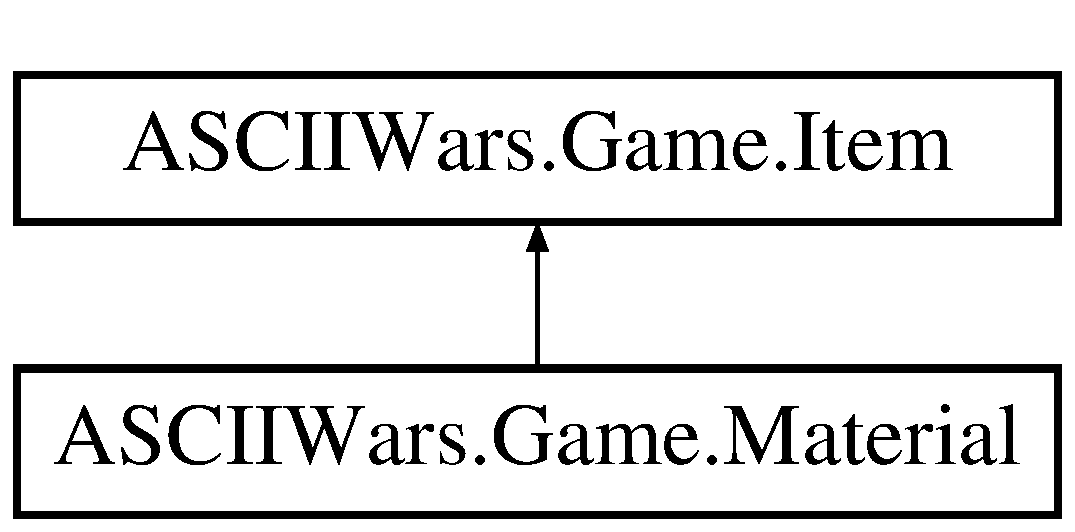
\includegraphics[height=2.000000cm]{class_a_s_c_i_i_wars_1_1_game_1_1_material}
\end{center}
\end{figure}
\subsection*{Открытые члены}
\begin{DoxyCompactItemize}
\item 
\hyperlink{class_a_s_c_i_i_wars_1_1_game_1_1_material_aa4aee4341c8099508c7ef1f980163e1d}{Material} (string \hyperlink{class_a_s_c_i_i_wars_1_1_game_1_1_item_a744d51f7684a4e46a1f834f8666db58e}{id}, string \hyperlink{class_a_s_c_i_i_wars_1_1_game_1_1_item_a994b9ec5f10c123e4345da159c090091}{name}, string \hyperlink{class_a_s_c_i_i_wars_1_1_game_1_1_item_a6ff41e953ccebc64a8df8f8c434535a0}{description})
\item 
override void \hyperlink{class_a_s_c_i_i_wars_1_1_game_1_1_material_afedb9d9b8b22782e40371b6cac37d27e}{On\+Add\+To\+Player\+Inventory} (\hyperlink{class_a_s_c_i_i_wars_1_1_game_1_1_player}{Player} player)
\item 
override void \hyperlink{class_a_s_c_i_i_wars_1_1_game_1_1_material_ab8467edc48ff6af4021f550c97cbec31}{On\+Remove\+From\+Player\+Inventory} (\hyperlink{class_a_s_c_i_i_wars_1_1_game_1_1_player}{Player} player)
\end{DoxyCompactItemize}
\subsection*{Дополнительные унаследованные члены}


\subsection{Конструктор(ы)}
\hypertarget{class_a_s_c_i_i_wars_1_1_game_1_1_material_aa4aee4341c8099508c7ef1f980163e1d}{}\label{class_a_s_c_i_i_wars_1_1_game_1_1_material_aa4aee4341c8099508c7ef1f980163e1d} 
\index{A\+S\+C\+I\+I\+Wars\+::\+Game\+::\+Material@{A\+S\+C\+I\+I\+Wars\+::\+Game\+::\+Material}!Material@{Material}}
\index{Material@{Material}!A\+S\+C\+I\+I\+Wars\+::\+Game\+::\+Material@{A\+S\+C\+I\+I\+Wars\+::\+Game\+::\+Material}}
\subsubsection{\texorpdfstring{Material()}{Material()}}
{\footnotesize\ttfamily A\+S\+C\+I\+I\+Wars.\+Game.\+Material.\+Material (\begin{DoxyParamCaption}\item[{string}]{id,  }\item[{string}]{name,  }\item[{string}]{description }\end{DoxyParamCaption})\hspace{0.3cm}{\ttfamily [inline]}}



\subsection{Методы}
\hypertarget{class_a_s_c_i_i_wars_1_1_game_1_1_material_afedb9d9b8b22782e40371b6cac37d27e}{}\label{class_a_s_c_i_i_wars_1_1_game_1_1_material_afedb9d9b8b22782e40371b6cac37d27e} 
\index{A\+S\+C\+I\+I\+Wars\+::\+Game\+::\+Material@{A\+S\+C\+I\+I\+Wars\+::\+Game\+::\+Material}!On\+Add\+To\+Player\+Inventory@{On\+Add\+To\+Player\+Inventory}}
\index{On\+Add\+To\+Player\+Inventory@{On\+Add\+To\+Player\+Inventory}!A\+S\+C\+I\+I\+Wars\+::\+Game\+::\+Material@{A\+S\+C\+I\+I\+Wars\+::\+Game\+::\+Material}}
\subsubsection{\texorpdfstring{On\+Add\+To\+Player\+Inventory()}{OnAddToPlayerInventory()}}
{\footnotesize\ttfamily override void A\+S\+C\+I\+I\+Wars.\+Game.\+Material.\+On\+Add\+To\+Player\+Inventory (\begin{DoxyParamCaption}\item[{\hyperlink{class_a_s_c_i_i_wars_1_1_game_1_1_player}{Player}}]{player }\end{DoxyParamCaption})\hspace{0.3cm}{\ttfamily [inline]}, {\ttfamily [virtual]}}



Замещает \hyperlink{class_a_s_c_i_i_wars_1_1_game_1_1_item_aec0355b7a9f647ef24897b95563f70d1}{A\+S\+C\+I\+I\+Wars.\+Game.\+Item}.

\hypertarget{class_a_s_c_i_i_wars_1_1_game_1_1_material_ab8467edc48ff6af4021f550c97cbec31}{}\label{class_a_s_c_i_i_wars_1_1_game_1_1_material_ab8467edc48ff6af4021f550c97cbec31} 
\index{A\+S\+C\+I\+I\+Wars\+::\+Game\+::\+Material@{A\+S\+C\+I\+I\+Wars\+::\+Game\+::\+Material}!On\+Remove\+From\+Player\+Inventory@{On\+Remove\+From\+Player\+Inventory}}
\index{On\+Remove\+From\+Player\+Inventory@{On\+Remove\+From\+Player\+Inventory}!A\+S\+C\+I\+I\+Wars\+::\+Game\+::\+Material@{A\+S\+C\+I\+I\+Wars\+::\+Game\+::\+Material}}
\subsubsection{\texorpdfstring{On\+Remove\+From\+Player\+Inventory()}{OnRemoveFromPlayerInventory()}}
{\footnotesize\ttfamily override void A\+S\+C\+I\+I\+Wars.\+Game.\+Material.\+On\+Remove\+From\+Player\+Inventory (\begin{DoxyParamCaption}\item[{\hyperlink{class_a_s_c_i_i_wars_1_1_game_1_1_player}{Player}}]{player }\end{DoxyParamCaption})\hspace{0.3cm}{\ttfamily [inline]}, {\ttfamily [virtual]}}



Замещает \hyperlink{class_a_s_c_i_i_wars_1_1_game_1_1_item_a52412546f837bfc65a3aa9d728fa142f}{A\+S\+C\+I\+I\+Wars.\+Game.\+Item}.



Объявления и описания членов класса находятся в файле\+:\begin{DoxyCompactItemize}
\item 
A\+S\+C\+I\+I\+Wars/\+Game/\hyperlink{_player_8cs}{Player.\+cs}\end{DoxyCompactItemize}

\hypertarget{class_a_s_c_i_i_wars_1_1_game_1_1_merchant}{}\section{Класс A\+S\+C\+I\+I\+Wars.\+Game.\+Merchant}
\label{class_a_s_c_i_i_wars_1_1_game_1_1_merchant}\index{A\+S\+C\+I\+I\+Wars.\+Game.\+Merchant@{A\+S\+C\+I\+I\+Wars.\+Game.\+Merchant}}
\subsection*{Открытые атрибуты}
\begin{DoxyCompactItemize}
\item 
string \hyperlink{class_a_s_c_i_i_wars_1_1_game_1_1_merchant_a6cc3b433c5be3021a26bdab57d9534e8}{id}
\item 
string \hyperlink{class_a_s_c_i_i_wars_1_1_game_1_1_merchant_ada225b0cd9c12c73b70729b821541d90}{name}
\item 
string \hyperlink{class_a_s_c_i_i_wars_1_1_game_1_1_merchant_a49fe8caa978e4dd0199f0b583f1c99a3}{type}
\item 
List$<$ \hyperlink{class_a_s_c_i_i_wars_1_1_game_1_1_merchant_item}{Merchant\+Item} $>$ \hyperlink{class_a_s_c_i_i_wars_1_1_game_1_1_merchant_aa35fa4b7dabae111e0819b68866fceba}{items}
\item 
List$<$ string $>$ \hyperlink{class_a_s_c_i_i_wars_1_1_game_1_1_merchant_a882142ada4b87c08a3a6b9e1c895c7c0}{next\+Situations}
\end{DoxyCompactItemize}


\subsection{Данные класса}
\hypertarget{class_a_s_c_i_i_wars_1_1_game_1_1_merchant_a6cc3b433c5be3021a26bdab57d9534e8}{}\label{class_a_s_c_i_i_wars_1_1_game_1_1_merchant_a6cc3b433c5be3021a26bdab57d9534e8} 
\index{A\+S\+C\+I\+I\+Wars\+::\+Game\+::\+Merchant@{A\+S\+C\+I\+I\+Wars\+::\+Game\+::\+Merchant}!id@{id}}
\index{id@{id}!A\+S\+C\+I\+I\+Wars\+::\+Game\+::\+Merchant@{A\+S\+C\+I\+I\+Wars\+::\+Game\+::\+Merchant}}
\subsubsection{\texorpdfstring{id}{id}}
{\footnotesize\ttfamily string A\+S\+C\+I\+I\+Wars.\+Game.\+Merchant.\+id}

\hypertarget{class_a_s_c_i_i_wars_1_1_game_1_1_merchant_aa35fa4b7dabae111e0819b68866fceba}{}\label{class_a_s_c_i_i_wars_1_1_game_1_1_merchant_aa35fa4b7dabae111e0819b68866fceba} 
\index{A\+S\+C\+I\+I\+Wars\+::\+Game\+::\+Merchant@{A\+S\+C\+I\+I\+Wars\+::\+Game\+::\+Merchant}!items@{items}}
\index{items@{items}!A\+S\+C\+I\+I\+Wars\+::\+Game\+::\+Merchant@{A\+S\+C\+I\+I\+Wars\+::\+Game\+::\+Merchant}}
\subsubsection{\texorpdfstring{items}{items}}
{\footnotesize\ttfamily List$<$\hyperlink{class_a_s_c_i_i_wars_1_1_game_1_1_merchant_item}{Merchant\+Item}$>$ A\+S\+C\+I\+I\+Wars.\+Game.\+Merchant.\+items}

\hypertarget{class_a_s_c_i_i_wars_1_1_game_1_1_merchant_ada225b0cd9c12c73b70729b821541d90}{}\label{class_a_s_c_i_i_wars_1_1_game_1_1_merchant_ada225b0cd9c12c73b70729b821541d90} 
\index{A\+S\+C\+I\+I\+Wars\+::\+Game\+::\+Merchant@{A\+S\+C\+I\+I\+Wars\+::\+Game\+::\+Merchant}!name@{name}}
\index{name@{name}!A\+S\+C\+I\+I\+Wars\+::\+Game\+::\+Merchant@{A\+S\+C\+I\+I\+Wars\+::\+Game\+::\+Merchant}}
\subsubsection{\texorpdfstring{name}{name}}
{\footnotesize\ttfamily string A\+S\+C\+I\+I\+Wars.\+Game.\+Merchant.\+name}

\hypertarget{class_a_s_c_i_i_wars_1_1_game_1_1_merchant_a882142ada4b87c08a3a6b9e1c895c7c0}{}\label{class_a_s_c_i_i_wars_1_1_game_1_1_merchant_a882142ada4b87c08a3a6b9e1c895c7c0} 
\index{A\+S\+C\+I\+I\+Wars\+::\+Game\+::\+Merchant@{A\+S\+C\+I\+I\+Wars\+::\+Game\+::\+Merchant}!next\+Situations@{next\+Situations}}
\index{next\+Situations@{next\+Situations}!A\+S\+C\+I\+I\+Wars\+::\+Game\+::\+Merchant@{A\+S\+C\+I\+I\+Wars\+::\+Game\+::\+Merchant}}
\subsubsection{\texorpdfstring{next\+Situations}{nextSituations}}
{\footnotesize\ttfamily List$<$string$>$ A\+S\+C\+I\+I\+Wars.\+Game.\+Merchant.\+next\+Situations}

\hypertarget{class_a_s_c_i_i_wars_1_1_game_1_1_merchant_a49fe8caa978e4dd0199f0b583f1c99a3}{}\label{class_a_s_c_i_i_wars_1_1_game_1_1_merchant_a49fe8caa978e4dd0199f0b583f1c99a3} 
\index{A\+S\+C\+I\+I\+Wars\+::\+Game\+::\+Merchant@{A\+S\+C\+I\+I\+Wars\+::\+Game\+::\+Merchant}!type@{type}}
\index{type@{type}!A\+S\+C\+I\+I\+Wars\+::\+Game\+::\+Merchant@{A\+S\+C\+I\+I\+Wars\+::\+Game\+::\+Merchant}}
\subsubsection{\texorpdfstring{type}{type}}
{\footnotesize\ttfamily string A\+S\+C\+I\+I\+Wars.\+Game.\+Merchant.\+type}



Объявления и описания членов класса находятся в файле\+:\begin{DoxyCompactItemize}
\item 
A\+S\+C\+I\+I\+Wars/\+Game/\hyperlink{_situations_8cs}{Situations.\+cs}\end{DoxyCompactItemize}

\hypertarget{class_a_s_c_i_i_wars_1_1_game_1_1_merchant_item}{}\section{Класс A\+S\+C\+I\+I\+Wars.\+Game.\+Merchant\+Item}
\label{class_a_s_c_i_i_wars_1_1_game_1_1_merchant_item}\index{A\+S\+C\+I\+I\+Wars.\+Game.\+Merchant\+Item@{A\+S\+C\+I\+I\+Wars.\+Game.\+Merchant\+Item}}
\subsection*{Открытые атрибуты}
\begin{DoxyCompactItemize}
\item 
string \hyperlink{class_a_s_c_i_i_wars_1_1_game_1_1_merchant_item_a43704fae44c4c55cb243bb6922558e12}{id}
\item 
string \hyperlink{class_a_s_c_i_i_wars_1_1_game_1_1_merchant_item_a0621b09ff9dc3029f660e32b90db815c}{type}
\item 
int \hyperlink{class_a_s_c_i_i_wars_1_1_game_1_1_merchant_item_af1b4ca7cc021067017ece68cc0145631}{price}
\end{DoxyCompactItemize}


\subsection{Данные класса}
\hypertarget{class_a_s_c_i_i_wars_1_1_game_1_1_merchant_item_a43704fae44c4c55cb243bb6922558e12}{}\label{class_a_s_c_i_i_wars_1_1_game_1_1_merchant_item_a43704fae44c4c55cb243bb6922558e12} 
\index{A\+S\+C\+I\+I\+Wars\+::\+Game\+::\+Merchant\+Item@{A\+S\+C\+I\+I\+Wars\+::\+Game\+::\+Merchant\+Item}!id@{id}}
\index{id@{id}!A\+S\+C\+I\+I\+Wars\+::\+Game\+::\+Merchant\+Item@{A\+S\+C\+I\+I\+Wars\+::\+Game\+::\+Merchant\+Item}}
\subsubsection{\texorpdfstring{id}{id}}
{\footnotesize\ttfamily string A\+S\+C\+I\+I\+Wars.\+Game.\+Merchant\+Item.\+id}

\hypertarget{class_a_s_c_i_i_wars_1_1_game_1_1_merchant_item_af1b4ca7cc021067017ece68cc0145631}{}\label{class_a_s_c_i_i_wars_1_1_game_1_1_merchant_item_af1b4ca7cc021067017ece68cc0145631} 
\index{A\+S\+C\+I\+I\+Wars\+::\+Game\+::\+Merchant\+Item@{A\+S\+C\+I\+I\+Wars\+::\+Game\+::\+Merchant\+Item}!price@{price}}
\index{price@{price}!A\+S\+C\+I\+I\+Wars\+::\+Game\+::\+Merchant\+Item@{A\+S\+C\+I\+I\+Wars\+::\+Game\+::\+Merchant\+Item}}
\subsubsection{\texorpdfstring{price}{price}}
{\footnotesize\ttfamily int A\+S\+C\+I\+I\+Wars.\+Game.\+Merchant\+Item.\+price}

\hypertarget{class_a_s_c_i_i_wars_1_1_game_1_1_merchant_item_a0621b09ff9dc3029f660e32b90db815c}{}\label{class_a_s_c_i_i_wars_1_1_game_1_1_merchant_item_a0621b09ff9dc3029f660e32b90db815c} 
\index{A\+S\+C\+I\+I\+Wars\+::\+Game\+::\+Merchant\+Item@{A\+S\+C\+I\+I\+Wars\+::\+Game\+::\+Merchant\+Item}!type@{type}}
\index{type@{type}!A\+S\+C\+I\+I\+Wars\+::\+Game\+::\+Merchant\+Item@{A\+S\+C\+I\+I\+Wars\+::\+Game\+::\+Merchant\+Item}}
\subsubsection{\texorpdfstring{type}{type}}
{\footnotesize\ttfamily string A\+S\+C\+I\+I\+Wars.\+Game.\+Merchant\+Item.\+type}



Объявления и описания членов класса находятся в файле\+:\begin{DoxyCompactItemize}
\item 
A\+S\+C\+I\+I\+Wars/\+Game/\hyperlink{_situations_8cs}{Situations.\+cs}\end{DoxyCompactItemize}

\hypertarget{class_a_s_c_i_i_wars_1_1_game_1_1_next_situation}{}\section{Класс A\+S\+C\+I\+I\+Wars.\+Game.\+Next\+Situation}
\label{class_a_s_c_i_i_wars_1_1_game_1_1_next_situation}\index{A\+S\+C\+I\+I\+Wars.\+Game.\+Next\+Situation@{A\+S\+C\+I\+I\+Wars.\+Game.\+Next\+Situation}}
\subsection*{Открытые атрибуты}
\begin{DoxyCompactItemize}
\item 
string \hyperlink{class_a_s_c_i_i_wars_1_1_game_1_1_next_situation_a5d21d7465e8bb363277591d61759ba1d}{title}
\item 
List$<$ string $>$ \hyperlink{class_a_s_c_i_i_wars_1_1_game_1_1_next_situation_a882f10c3c66963ef3e67c9e30689c968}{I\+Ds}
\end{DoxyCompactItemize}


\subsection{Данные класса}
\hypertarget{class_a_s_c_i_i_wars_1_1_game_1_1_next_situation_a882f10c3c66963ef3e67c9e30689c968}{}\label{class_a_s_c_i_i_wars_1_1_game_1_1_next_situation_a882f10c3c66963ef3e67c9e30689c968} 
\index{A\+S\+C\+I\+I\+Wars\+::\+Game\+::\+Next\+Situation@{A\+S\+C\+I\+I\+Wars\+::\+Game\+::\+Next\+Situation}!I\+Ds@{I\+Ds}}
\index{I\+Ds@{I\+Ds}!A\+S\+C\+I\+I\+Wars\+::\+Game\+::\+Next\+Situation@{A\+S\+C\+I\+I\+Wars\+::\+Game\+::\+Next\+Situation}}
\subsubsection{\texorpdfstring{I\+Ds}{IDs}}
{\footnotesize\ttfamily List$<$string$>$ A\+S\+C\+I\+I\+Wars.\+Game.\+Next\+Situation.\+I\+Ds}

\hypertarget{class_a_s_c_i_i_wars_1_1_game_1_1_next_situation_a5d21d7465e8bb363277591d61759ba1d}{}\label{class_a_s_c_i_i_wars_1_1_game_1_1_next_situation_a5d21d7465e8bb363277591d61759ba1d} 
\index{A\+S\+C\+I\+I\+Wars\+::\+Game\+::\+Next\+Situation@{A\+S\+C\+I\+I\+Wars\+::\+Game\+::\+Next\+Situation}!title@{title}}
\index{title@{title}!A\+S\+C\+I\+I\+Wars\+::\+Game\+::\+Next\+Situation@{A\+S\+C\+I\+I\+Wars\+::\+Game\+::\+Next\+Situation}}
\subsubsection{\texorpdfstring{title}{title}}
{\footnotesize\ttfamily string A\+S\+C\+I\+I\+Wars.\+Game.\+Next\+Situation.\+title}



Объявления и описания членов класса находятся в файле\+:\begin{DoxyCompactItemize}
\item 
A\+S\+C\+I\+I\+Wars/\+Game/\hyperlink{_situations_8cs}{Situations.\+cs}\end{DoxyCompactItemize}

\hypertarget{class_a_s_c_i_i_wars_1_1_game_1_1_player}{}\section{Класс A\+S\+C\+I\+I\+Wars.\+Game.\+Player}
\label{class_a_s_c_i_i_wars_1_1_game_1_1_player}\index{A\+S\+C\+I\+I\+Wars.\+Game.\+Player@{A\+S\+C\+I\+I\+Wars.\+Game.\+Player}}


Представляет игрока.  


\subsection*{Открытые члены}
\begin{DoxyCompactItemize}
\item 
void \hyperlink{class_a_s_c_i_i_wars_1_1_game_1_1_player_a51054cd802e781a9f0a018f893ec3877}{Add\+Item\+To\+Inventory} (\hyperlink{class_a_s_c_i_i_wars_1_1_game_1_1_item}{Item} item)
\begin{DoxyCompactList}\small\item\em Добавляет предмет в инвентарь, с учётом максимального размера. \end{DoxyCompactList}\item 
void \hyperlink{class_a_s_c_i_i_wars_1_1_game_1_1_player_a7c362d28cd4146ebdcebc754982c0ad8}{Add\+Item\+To\+Inventory} (\hyperlink{class_a_s_c_i_i_wars_1_1_game_1_1_item}{Item} item, int count)
\item 
void \hyperlink{class_a_s_c_i_i_wars_1_1_game_1_1_player_aa58a605f6337c385f4023ea842f6c246}{Remove\+Item\+From\+Inventory} (\hyperlink{class_a_s_c_i_i_wars_1_1_game_1_1_item}{Item} item)
\begin{DoxyCompactList}\small\item\em Удаляет предмет из инвентаря. \end{DoxyCompactList}\item 
void \hyperlink{class_a_s_c_i_i_wars_1_1_game_1_1_player_acef087ca862c4f210d7d049a2b09b29f}{Remove\+Item\+From\+Inventory} (\hyperlink{class_a_s_c_i_i_wars_1_1_game_1_1_item}{Item} item, int count)
\item 
void \hyperlink{class_a_s_c_i_i_wars_1_1_game_1_1_player_aec1c1f808fa3da1585a62487b0e92a38}{Select\+Item\+In\+Inventory} (\hyperlink{class_a_s_c_i_i_wars_1_1_game_1_1_selectable}{Selectable} selectable)
\begin{DoxyCompactList}\small\item\em Выбирает выбираемый предмет в инвентаре, и отключает уже выбраный предмет этого типа. \end{DoxyCompactList}\item 
void \hyperlink{class_a_s_c_i_i_wars_1_1_game_1_1_player_a104ae32d59b6e627d55dc78ff4ffa995}{Deselect\+Item\+In\+Inventory} (\hyperlink{class_a_s_c_i_i_wars_1_1_game_1_1_selectable}{Selectable} selectable)
\begin{DoxyCompactList}\small\item\em Отключает выбираемый предмет в инвентаре. \end{DoxyCompactList}\item 
void \hyperlink{class_a_s_c_i_i_wars_1_1_game_1_1_player_ac1b40c126e1d9ec4f45f7831a86497ba}{Consume\+Item\+From\+Inventory} (\hyperlink{class_a_s_c_i_i_wars_1_1_game_1_1_consumable}{Consumable} consumable)
\begin{DoxyCompactList}\small\item\em Использует и удаляет используемый предмет в инвентаре. \end{DoxyCompactList}\item 
int \hyperlink{class_a_s_c_i_i_wars_1_1_game_1_1_player_acb07b9e02dfe26cae85c1b685517438b}{Count\+Of\+Item\+In\+Inventory} (\hyperlink{class_a_s_c_i_i_wars_1_1_game_1_1_item}{Item} item)
\begin{DoxyCompactList}\small\item\em Возвращает число предметов определённого типа в инвентаре. \end{DoxyCompactList}\end{DoxyCompactItemize}
\subsection*{Открытые атрибуты}
\begin{DoxyCompactItemize}
\item 
const int \hyperlink{class_a_s_c_i_i_wars_1_1_game_1_1_player_a1cc8a05398a717bcf8c5a0ebd2ea0747}{M\+A\+X\+\_\+\+I\+N\+V\+E\+N\+T\+O\+R\+Y\+\_\+\+S\+I\+ZE} = 20
\begin{DoxyCompactList}\small\item\em Максимальный размер инвентаря. \end{DoxyCompactList}\item 
int \hyperlink{class_a_s_c_i_i_wars_1_1_game_1_1_player_acfd121f865f0e5a87f177e93c82feadc}{max\+Health} = \hyperlink{class_a_s_c_i_i_wars_1_1_game_1_1_player_ab5921985db319187e317563c15ef48dc}{D\+E\+F\+A\+U\+L\+T\+\_\+\+M\+A\+X\+\_\+\+H\+E\+A\+L\+TH}
\begin{DoxyCompactList}\small\item\em Максимальное здоровье. Может увеличиваться в течении игры с помощью \hyperlink{class_a_s_c_i_i_wars_1_1_game_1_1_health_booster}{A\+S\+C\+I\+I\+Wars.\+Game.\+Health\+Booster}. \end{DoxyCompactList}\item 
int \hyperlink{class_a_s_c_i_i_wars_1_1_game_1_1_player_a8f364a47ef452b6c99bc13b7bdaae7ca}{health} = \hyperlink{class_a_s_c_i_i_wars_1_1_game_1_1_player_ab5921985db319187e317563c15ef48dc}{D\+E\+F\+A\+U\+L\+T\+\_\+\+M\+A\+X\+\_\+\+H\+E\+A\+L\+TH}
\begin{DoxyCompactList}\small\item\em Уровень здоровья. Может регенерироваться в течении игры с помощью \hyperlink{class_a_s_c_i_i_wars_1_1_game_1_1_health_potion}{A\+S\+C\+I\+I\+Wars.\+Game.\+Health\+Potion}. \end{DoxyCompactList}\item 
int \hyperlink{class_a_s_c_i_i_wars_1_1_game_1_1_player_a45736ed2f9941e3877df09db83cd4032}{attack}
\begin{DoxyCompactList}\small\item\em Уровень атаки. Может увеличиваться в течении игры с помощью \hyperlink{class_a_s_c_i_i_wars_1_1_game_1_1_weapon}{A\+S\+C\+I\+I\+Wars.\+Game.\+Weapon}. \end{DoxyCompactList}\item 
int \hyperlink{class_a_s_c_i_i_wars_1_1_game_1_1_player_a1dc39c7d8054c42dcb7af70e78b3be02}{defense}
\begin{DoxyCompactList}\small\item\em Уровень защиты. Может увеличиваться в течении игры с помощью \hyperlink{class_a_s_c_i_i_wars_1_1_game_1_1_armor}{A\+S\+C\+I\+I\+Wars.\+Game.\+Armor}. \end{DoxyCompactList}\item 
int \hyperlink{class_a_s_c_i_i_wars_1_1_game_1_1_player_a5abede19c5428143df924357ad475691}{coins} = \hyperlink{class_a_s_c_i_i_wars_1_1_game_1_1_player_af33b6af0d723918290a4a38aa4a6fb66}{S\+T\+A\+R\+T\+E\+R\+\_\+\+C\+O\+I\+NS}
\begin{DoxyCompactList}\small\item\em Количество монет у игрока. \end{DoxyCompactList}\item 
List$<$ \hyperlink{class_a_s_c_i_i_wars_1_1_game_1_1_item}{Item} $>$ \hyperlink{class_a_s_c_i_i_wars_1_1_game_1_1_player_a04acfaa196162f89bfae7aee5ec45480}{inventory} = new List$<$\hyperlink{class_a_s_c_i_i_wars_1_1_game_1_1_item}{Item}$>$()
\begin{DoxyCompactList}\small\item\em Инвентарь. Имеет ограничение по размеру (\hyperlink{class_a_s_c_i_i_wars_1_1_game_1_1_player_a1cc8a05398a717bcf8c5a0ebd2ea0747}{M\+A\+X\+\_\+\+I\+N\+V\+E\+N\+T\+O\+R\+Y\+\_\+\+S\+I\+ZE}). \end{DoxyCompactList}\end{DoxyCompactItemize}
\subsection*{Закрытые данные}
\begin{DoxyCompactItemize}
\item 
const int \hyperlink{class_a_s_c_i_i_wars_1_1_game_1_1_player_ab5921985db319187e317563c15ef48dc}{D\+E\+F\+A\+U\+L\+T\+\_\+\+M\+A\+X\+\_\+\+H\+E\+A\+L\+TH} = 100
\begin{DoxyCompactList}\small\item\em Максимальное значение здоровья по умолчанию. \end{DoxyCompactList}\item 
const int \hyperlink{class_a_s_c_i_i_wars_1_1_game_1_1_player_af33b6af0d723918290a4a38aa4a6fb66}{S\+T\+A\+R\+T\+E\+R\+\_\+\+C\+O\+I\+NS} = 10
\begin{DoxyCompactList}\small\item\em Количество монет в начале игры. \end{DoxyCompactList}\end{DoxyCompactItemize}


\subsection{Подробное описание}
Представляет игрока. 

У игрока есть такие свойства\+:
\begin{DoxyItemize}
\item здоровье (\hyperlink{class_a_s_c_i_i_wars_1_1_game_1_1_player_a8f364a47ef452b6c99bc13b7bdaae7ca}{health})
\begin{DoxyItemize}
\item Ограничено максимальным значением (\hyperlink{class_a_s_c_i_i_wars_1_1_game_1_1_player_acfd121f865f0e5a87f177e93c82feadc}{max\+Health}), которое может увеличиваться (с помощью \hyperlink{class_a_s_c_i_i_wars_1_1_game_1_1_health_booster}{A\+S\+C\+I\+I\+Wars.\+Game.\+Health\+Booster})
\end{DoxyItemize}
\item атака (\hyperlink{class_a_s_c_i_i_wars_1_1_game_1_1_player_a45736ed2f9941e3877df09db83cd4032}{attack})
\item защита (\hyperlink{class_a_s_c_i_i_wars_1_1_game_1_1_player_a1dc39c7d8054c42dcb7af70e78b3be02}{defense})
\item инвентарь (\hyperlink{class_a_s_c_i_i_wars_1_1_game_1_1_player_a04acfaa196162f89bfae7aee5ec45480}{inventory})
\begin{DoxyItemize}
\item Размер ограничнен максимальным значением (\hyperlink{class_a_s_c_i_i_wars_1_1_game_1_1_player_a1cc8a05398a717bcf8c5a0ebd2ea0747}{M\+A\+X\+\_\+\+I\+N\+V\+E\+N\+T\+O\+R\+Y\+\_\+\+S\+I\+ZE}), которое не может увеличиваться
\end{DoxyItemize}
\item монеты (\hyperlink{class_a_s_c_i_i_wars_1_1_game_1_1_player_a5abede19c5428143df924357ad475691}{coins})
\begin{DoxyItemize}
\item В начале игры даётся определённое количиство монет (\hyperlink{class_a_s_c_i_i_wars_1_1_game_1_1_player_af33b6af0d723918290a4a38aa4a6fb66}{S\+T\+A\+R\+T\+E\+R\+\_\+\+C\+O\+I\+NS}) 
\end{DoxyItemize}
\end{DoxyItemize}

\subsection{Методы}
\hypertarget{class_a_s_c_i_i_wars_1_1_game_1_1_player_a51054cd802e781a9f0a018f893ec3877}{}\label{class_a_s_c_i_i_wars_1_1_game_1_1_player_a51054cd802e781a9f0a018f893ec3877} 
\index{A\+S\+C\+I\+I\+Wars\+::\+Game\+::\+Player@{A\+S\+C\+I\+I\+Wars\+::\+Game\+::\+Player}!Add\+Item\+To\+Inventory@{Add\+Item\+To\+Inventory}}
\index{Add\+Item\+To\+Inventory@{Add\+Item\+To\+Inventory}!A\+S\+C\+I\+I\+Wars\+::\+Game\+::\+Player@{A\+S\+C\+I\+I\+Wars\+::\+Game\+::\+Player}}
\subsubsection{\texorpdfstring{Add\+Item\+To\+Inventory()}{AddItemToInventory()}\hspace{0.1cm}{\footnotesize\ttfamily [1/2]}}
{\footnotesize\ttfamily void A\+S\+C\+I\+I\+Wars.\+Game.\+Player.\+Add\+Item\+To\+Inventory (\begin{DoxyParamCaption}\item[{\hyperlink{class_a_s_c_i_i_wars_1_1_game_1_1_item}{Item}}]{item }\end{DoxyParamCaption})\hspace{0.3cm}{\ttfamily [inline]}}



Добавляет предмет в инвентарь, с учётом максимального размера. 

\begin{DoxySeeAlso}{См. также}
\hyperlink{class_a_s_c_i_i_wars_1_1_game_1_1_player_a04acfaa196162f89bfae7aee5ec45480}{inventory} 

\hyperlink{class_a_s_c_i_i_wars_1_1_game_1_1_item}{Item} 

\hyperlink{class_a_s_c_i_i_wars_1_1_game_1_1_item_aec0355b7a9f647ef24897b95563f70d1}{Item.\+On\+Add\+To\+Player\+Inventory(\+Player)} 

\hyperlink{class_a_s_c_i_i_wars_1_1_game_1_1_player_aa58a605f6337c385f4023ea842f6c246}{Remove\+Item\+From\+Inventory(\+Item)} 
\end{DoxySeeAlso}
\hypertarget{class_a_s_c_i_i_wars_1_1_game_1_1_player_a7c362d28cd4146ebdcebc754982c0ad8}{}\label{class_a_s_c_i_i_wars_1_1_game_1_1_player_a7c362d28cd4146ebdcebc754982c0ad8} 
\index{A\+S\+C\+I\+I\+Wars\+::\+Game\+::\+Player@{A\+S\+C\+I\+I\+Wars\+::\+Game\+::\+Player}!Add\+Item\+To\+Inventory@{Add\+Item\+To\+Inventory}}
\index{Add\+Item\+To\+Inventory@{Add\+Item\+To\+Inventory}!A\+S\+C\+I\+I\+Wars\+::\+Game\+::\+Player@{A\+S\+C\+I\+I\+Wars\+::\+Game\+::\+Player}}
\subsubsection{\texorpdfstring{Add\+Item\+To\+Inventory()}{AddItemToInventory()}\hspace{0.1cm}{\footnotesize\ttfamily [2/2]}}
{\footnotesize\ttfamily void A\+S\+C\+I\+I\+Wars.\+Game.\+Player.\+Add\+Item\+To\+Inventory (\begin{DoxyParamCaption}\item[{\hyperlink{class_a_s_c_i_i_wars_1_1_game_1_1_item}{Item}}]{item,  }\item[{int}]{count }\end{DoxyParamCaption})\hspace{0.3cm}{\ttfamily [inline]}}

\hypertarget{class_a_s_c_i_i_wars_1_1_game_1_1_player_ac1b40c126e1d9ec4f45f7831a86497ba}{}\label{class_a_s_c_i_i_wars_1_1_game_1_1_player_ac1b40c126e1d9ec4f45f7831a86497ba} 
\index{A\+S\+C\+I\+I\+Wars\+::\+Game\+::\+Player@{A\+S\+C\+I\+I\+Wars\+::\+Game\+::\+Player}!Consume\+Item\+From\+Inventory@{Consume\+Item\+From\+Inventory}}
\index{Consume\+Item\+From\+Inventory@{Consume\+Item\+From\+Inventory}!A\+S\+C\+I\+I\+Wars\+::\+Game\+::\+Player@{A\+S\+C\+I\+I\+Wars\+::\+Game\+::\+Player}}
\subsubsection{\texorpdfstring{Consume\+Item\+From\+Inventory()}{ConsumeItemFromInventory()}}
{\footnotesize\ttfamily void A\+S\+C\+I\+I\+Wars.\+Game.\+Player.\+Consume\+Item\+From\+Inventory (\begin{DoxyParamCaption}\item[{\hyperlink{class_a_s_c_i_i_wars_1_1_game_1_1_consumable}{Consumable}}]{consumable }\end{DoxyParamCaption})\hspace{0.3cm}{\ttfamily [inline]}}



Использует и удаляет используемый предмет в инвентаре. 

\begin{DoxySeeAlso}{См. также}
\hyperlink{class_a_s_c_i_i_wars_1_1_game_1_1_player_a04acfaa196162f89bfae7aee5ec45480}{inventory} 

\hyperlink{class_a_s_c_i_i_wars_1_1_game_1_1_consumable}{Consumable} 

\hyperlink{class_a_s_c_i_i_wars_1_1_game_1_1_consumable_a6aac67fe076ca39cb850e3720461fff8}{Consumable.\+On\+Consume\+By\+Player(\+Player)} 
\end{DoxySeeAlso}
\hypertarget{class_a_s_c_i_i_wars_1_1_game_1_1_player_acb07b9e02dfe26cae85c1b685517438b}{}\label{class_a_s_c_i_i_wars_1_1_game_1_1_player_acb07b9e02dfe26cae85c1b685517438b} 
\index{A\+S\+C\+I\+I\+Wars\+::\+Game\+::\+Player@{A\+S\+C\+I\+I\+Wars\+::\+Game\+::\+Player}!Count\+Of\+Item\+In\+Inventory@{Count\+Of\+Item\+In\+Inventory}}
\index{Count\+Of\+Item\+In\+Inventory@{Count\+Of\+Item\+In\+Inventory}!A\+S\+C\+I\+I\+Wars\+::\+Game\+::\+Player@{A\+S\+C\+I\+I\+Wars\+::\+Game\+::\+Player}}
\subsubsection{\texorpdfstring{Count\+Of\+Item\+In\+Inventory()}{CountOfItemInInventory()}}
{\footnotesize\ttfamily int A\+S\+C\+I\+I\+Wars.\+Game.\+Player.\+Count\+Of\+Item\+In\+Inventory (\begin{DoxyParamCaption}\item[{\hyperlink{class_a_s_c_i_i_wars_1_1_game_1_1_item}{Item}}]{item }\end{DoxyParamCaption})\hspace{0.3cm}{\ttfamily [inline]}}



Возвращает число предметов определённого типа в инвентаре. 

\begin{DoxySeeAlso}{См. также}
\hyperlink{class_a_s_c_i_i_wars_1_1_game_1_1_player_a04acfaa196162f89bfae7aee5ec45480}{inventory} 
\end{DoxySeeAlso}
\hypertarget{class_a_s_c_i_i_wars_1_1_game_1_1_player_a104ae32d59b6e627d55dc78ff4ffa995}{}\label{class_a_s_c_i_i_wars_1_1_game_1_1_player_a104ae32d59b6e627d55dc78ff4ffa995} 
\index{A\+S\+C\+I\+I\+Wars\+::\+Game\+::\+Player@{A\+S\+C\+I\+I\+Wars\+::\+Game\+::\+Player}!Deselect\+Item\+In\+Inventory@{Deselect\+Item\+In\+Inventory}}
\index{Deselect\+Item\+In\+Inventory@{Deselect\+Item\+In\+Inventory}!A\+S\+C\+I\+I\+Wars\+::\+Game\+::\+Player@{A\+S\+C\+I\+I\+Wars\+::\+Game\+::\+Player}}
\subsubsection{\texorpdfstring{Deselect\+Item\+In\+Inventory()}{DeselectItemInInventory()}}
{\footnotesize\ttfamily void A\+S\+C\+I\+I\+Wars.\+Game.\+Player.\+Deselect\+Item\+In\+Inventory (\begin{DoxyParamCaption}\item[{\hyperlink{class_a_s_c_i_i_wars_1_1_game_1_1_selectable}{Selectable}}]{selectable }\end{DoxyParamCaption})\hspace{0.3cm}{\ttfamily [inline]}}



Отключает выбираемый предмет в инвентаре. 

\begin{DoxySeeAlso}{См. также}
\hyperlink{class_a_s_c_i_i_wars_1_1_game_1_1_player_a04acfaa196162f89bfae7aee5ec45480}{inventory} 

\hyperlink{class_a_s_c_i_i_wars_1_1_game_1_1_selectable}{Selectable} 

\hyperlink{class_a_s_c_i_i_wars_1_1_game_1_1_selectable_a08a30c8786367bf45355e989b109c44b}{Selectable.\+On\+Deselect\+By\+Player(\+Player)} 

\hyperlink{class_a_s_c_i_i_wars_1_1_game_1_1_player_aec1c1f808fa3da1585a62487b0e92a38}{Select\+Item\+In\+Inventory(\+Selectable)} 
\end{DoxySeeAlso}
\hypertarget{class_a_s_c_i_i_wars_1_1_game_1_1_player_aa58a605f6337c385f4023ea842f6c246}{}\label{class_a_s_c_i_i_wars_1_1_game_1_1_player_aa58a605f6337c385f4023ea842f6c246} 
\index{A\+S\+C\+I\+I\+Wars\+::\+Game\+::\+Player@{A\+S\+C\+I\+I\+Wars\+::\+Game\+::\+Player}!Remove\+Item\+From\+Inventory@{Remove\+Item\+From\+Inventory}}
\index{Remove\+Item\+From\+Inventory@{Remove\+Item\+From\+Inventory}!A\+S\+C\+I\+I\+Wars\+::\+Game\+::\+Player@{A\+S\+C\+I\+I\+Wars\+::\+Game\+::\+Player}}
\subsubsection{\texorpdfstring{Remove\+Item\+From\+Inventory()}{RemoveItemFromInventory()}\hspace{0.1cm}{\footnotesize\ttfamily [1/2]}}
{\footnotesize\ttfamily void A\+S\+C\+I\+I\+Wars.\+Game.\+Player.\+Remove\+Item\+From\+Inventory (\begin{DoxyParamCaption}\item[{\hyperlink{class_a_s_c_i_i_wars_1_1_game_1_1_item}{Item}}]{item }\end{DoxyParamCaption})\hspace{0.3cm}{\ttfamily [inline]}}



Удаляет предмет из инвентаря. 

\begin{DoxySeeAlso}{См. также}
\hyperlink{class_a_s_c_i_i_wars_1_1_game_1_1_player_a04acfaa196162f89bfae7aee5ec45480}{inventory} 

\hyperlink{class_a_s_c_i_i_wars_1_1_game_1_1_item}{Item} 

\hyperlink{class_a_s_c_i_i_wars_1_1_game_1_1_item_a52412546f837bfc65a3aa9d728fa142f}{Item.\+On\+Remove\+From\+Player\+Inventory(\+Player)} 

\hyperlink{class_a_s_c_i_i_wars_1_1_game_1_1_player_a51054cd802e781a9f0a018f893ec3877}{Add\+Item\+To\+Inventory(\+Item)} 
\end{DoxySeeAlso}
\hypertarget{class_a_s_c_i_i_wars_1_1_game_1_1_player_acef087ca862c4f210d7d049a2b09b29f}{}\label{class_a_s_c_i_i_wars_1_1_game_1_1_player_acef087ca862c4f210d7d049a2b09b29f} 
\index{A\+S\+C\+I\+I\+Wars\+::\+Game\+::\+Player@{A\+S\+C\+I\+I\+Wars\+::\+Game\+::\+Player}!Remove\+Item\+From\+Inventory@{Remove\+Item\+From\+Inventory}}
\index{Remove\+Item\+From\+Inventory@{Remove\+Item\+From\+Inventory}!A\+S\+C\+I\+I\+Wars\+::\+Game\+::\+Player@{A\+S\+C\+I\+I\+Wars\+::\+Game\+::\+Player}}
\subsubsection{\texorpdfstring{Remove\+Item\+From\+Inventory()}{RemoveItemFromInventory()}\hspace{0.1cm}{\footnotesize\ttfamily [2/2]}}
{\footnotesize\ttfamily void A\+S\+C\+I\+I\+Wars.\+Game.\+Player.\+Remove\+Item\+From\+Inventory (\begin{DoxyParamCaption}\item[{\hyperlink{class_a_s_c_i_i_wars_1_1_game_1_1_item}{Item}}]{item,  }\item[{int}]{count }\end{DoxyParamCaption})\hspace{0.3cm}{\ttfamily [inline]}}

\hypertarget{class_a_s_c_i_i_wars_1_1_game_1_1_player_aec1c1f808fa3da1585a62487b0e92a38}{}\label{class_a_s_c_i_i_wars_1_1_game_1_1_player_aec1c1f808fa3da1585a62487b0e92a38} 
\index{A\+S\+C\+I\+I\+Wars\+::\+Game\+::\+Player@{A\+S\+C\+I\+I\+Wars\+::\+Game\+::\+Player}!Select\+Item\+In\+Inventory@{Select\+Item\+In\+Inventory}}
\index{Select\+Item\+In\+Inventory@{Select\+Item\+In\+Inventory}!A\+S\+C\+I\+I\+Wars\+::\+Game\+::\+Player@{A\+S\+C\+I\+I\+Wars\+::\+Game\+::\+Player}}
\subsubsection{\texorpdfstring{Select\+Item\+In\+Inventory()}{SelectItemInInventory()}}
{\footnotesize\ttfamily void A\+S\+C\+I\+I\+Wars.\+Game.\+Player.\+Select\+Item\+In\+Inventory (\begin{DoxyParamCaption}\item[{\hyperlink{class_a_s_c_i_i_wars_1_1_game_1_1_selectable}{Selectable}}]{selectable }\end{DoxyParamCaption})\hspace{0.3cm}{\ttfamily [inline]}}



Выбирает выбираемый предмет в инвентаре, и отключает уже выбраный предмет этого типа. 

\begin{DoxySeeAlso}{См. также}
\hyperlink{class_a_s_c_i_i_wars_1_1_game_1_1_player_a04acfaa196162f89bfae7aee5ec45480}{inventory} 

\hyperlink{class_a_s_c_i_i_wars_1_1_game_1_1_selectable}{Selectable} 

\hyperlink{class_a_s_c_i_i_wars_1_1_game_1_1_selectable_a95bdcf05ef9ea5f39c81ddd96294968a}{Selectable.\+On\+Select\+By\+Player(\+Player)} 

\hyperlink{class_a_s_c_i_i_wars_1_1_game_1_1_player_a104ae32d59b6e627d55dc78ff4ffa995}{Deselect\+Item\+In\+Inventory(\+Selectable)} 
\end{DoxySeeAlso}


\subsection{Данные класса}
\hypertarget{class_a_s_c_i_i_wars_1_1_game_1_1_player_a45736ed2f9941e3877df09db83cd4032}{}\label{class_a_s_c_i_i_wars_1_1_game_1_1_player_a45736ed2f9941e3877df09db83cd4032} 
\index{A\+S\+C\+I\+I\+Wars\+::\+Game\+::\+Player@{A\+S\+C\+I\+I\+Wars\+::\+Game\+::\+Player}!attack@{attack}}
\index{attack@{attack}!A\+S\+C\+I\+I\+Wars\+::\+Game\+::\+Player@{A\+S\+C\+I\+I\+Wars\+::\+Game\+::\+Player}}
\subsubsection{\texorpdfstring{attack}{attack}}
{\footnotesize\ttfamily int A\+S\+C\+I\+I\+Wars.\+Game.\+Player.\+attack}



Уровень атаки. Может увеличиваться в течении игры с помощью \hyperlink{class_a_s_c_i_i_wars_1_1_game_1_1_weapon}{A\+S\+C\+I\+I\+Wars.\+Game.\+Weapon}. 

\hypertarget{class_a_s_c_i_i_wars_1_1_game_1_1_player_a5abede19c5428143df924357ad475691}{}\label{class_a_s_c_i_i_wars_1_1_game_1_1_player_a5abede19c5428143df924357ad475691} 
\index{A\+S\+C\+I\+I\+Wars\+::\+Game\+::\+Player@{A\+S\+C\+I\+I\+Wars\+::\+Game\+::\+Player}!coins@{coins}}
\index{coins@{coins}!A\+S\+C\+I\+I\+Wars\+::\+Game\+::\+Player@{A\+S\+C\+I\+I\+Wars\+::\+Game\+::\+Player}}
\subsubsection{\texorpdfstring{coins}{coins}}
{\footnotesize\ttfamily int A\+S\+C\+I\+I\+Wars.\+Game.\+Player.\+coins = \hyperlink{class_a_s_c_i_i_wars_1_1_game_1_1_player_af33b6af0d723918290a4a38aa4a6fb66}{S\+T\+A\+R\+T\+E\+R\+\_\+\+C\+O\+I\+NS}}



Количество монет у игрока. 

\hypertarget{class_a_s_c_i_i_wars_1_1_game_1_1_player_ab5921985db319187e317563c15ef48dc}{}\label{class_a_s_c_i_i_wars_1_1_game_1_1_player_ab5921985db319187e317563c15ef48dc} 
\index{A\+S\+C\+I\+I\+Wars\+::\+Game\+::\+Player@{A\+S\+C\+I\+I\+Wars\+::\+Game\+::\+Player}!D\+E\+F\+A\+U\+L\+T\+\_\+\+M\+A\+X\+\_\+\+H\+E\+A\+L\+TH@{D\+E\+F\+A\+U\+L\+T\+\_\+\+M\+A\+X\+\_\+\+H\+E\+A\+L\+TH}}
\index{D\+E\+F\+A\+U\+L\+T\+\_\+\+M\+A\+X\+\_\+\+H\+E\+A\+L\+TH@{D\+E\+F\+A\+U\+L\+T\+\_\+\+M\+A\+X\+\_\+\+H\+E\+A\+L\+TH}!A\+S\+C\+I\+I\+Wars\+::\+Game\+::\+Player@{A\+S\+C\+I\+I\+Wars\+::\+Game\+::\+Player}}
\subsubsection{\texorpdfstring{D\+E\+F\+A\+U\+L\+T\+\_\+\+M\+A\+X\+\_\+\+H\+E\+A\+L\+TH}{DEFAULT\_MAX\_HEALTH}}
{\footnotesize\ttfamily const int A\+S\+C\+I\+I\+Wars.\+Game.\+Player.\+D\+E\+F\+A\+U\+L\+T\+\_\+\+M\+A\+X\+\_\+\+H\+E\+A\+L\+TH = 100\hspace{0.3cm}{\ttfamily [private]}}



Максимальное значение здоровья по умолчанию. 

\begin{DoxySeeAlso}{См. также}
\hyperlink{class_a_s_c_i_i_wars_1_1_game_1_1_player_acfd121f865f0e5a87f177e93c82feadc}{max\+Health} 
\end{DoxySeeAlso}
\hypertarget{class_a_s_c_i_i_wars_1_1_game_1_1_player_a1dc39c7d8054c42dcb7af70e78b3be02}{}\label{class_a_s_c_i_i_wars_1_1_game_1_1_player_a1dc39c7d8054c42dcb7af70e78b3be02} 
\index{A\+S\+C\+I\+I\+Wars\+::\+Game\+::\+Player@{A\+S\+C\+I\+I\+Wars\+::\+Game\+::\+Player}!defense@{defense}}
\index{defense@{defense}!A\+S\+C\+I\+I\+Wars\+::\+Game\+::\+Player@{A\+S\+C\+I\+I\+Wars\+::\+Game\+::\+Player}}
\subsubsection{\texorpdfstring{defense}{defense}}
{\footnotesize\ttfamily int A\+S\+C\+I\+I\+Wars.\+Game.\+Player.\+defense}



Уровень защиты. Может увеличиваться в течении игры с помощью \hyperlink{class_a_s_c_i_i_wars_1_1_game_1_1_armor}{A\+S\+C\+I\+I\+Wars.\+Game.\+Armor}. 

\hypertarget{class_a_s_c_i_i_wars_1_1_game_1_1_player_a8f364a47ef452b6c99bc13b7bdaae7ca}{}\label{class_a_s_c_i_i_wars_1_1_game_1_1_player_a8f364a47ef452b6c99bc13b7bdaae7ca} 
\index{A\+S\+C\+I\+I\+Wars\+::\+Game\+::\+Player@{A\+S\+C\+I\+I\+Wars\+::\+Game\+::\+Player}!health@{health}}
\index{health@{health}!A\+S\+C\+I\+I\+Wars\+::\+Game\+::\+Player@{A\+S\+C\+I\+I\+Wars\+::\+Game\+::\+Player}}
\subsubsection{\texorpdfstring{health}{health}}
{\footnotesize\ttfamily int A\+S\+C\+I\+I\+Wars.\+Game.\+Player.\+health = \hyperlink{class_a_s_c_i_i_wars_1_1_game_1_1_player_ab5921985db319187e317563c15ef48dc}{D\+E\+F\+A\+U\+L\+T\+\_\+\+M\+A\+X\+\_\+\+H\+E\+A\+L\+TH}}



Уровень здоровья. Может регенерироваться в течении игры с помощью \hyperlink{class_a_s_c_i_i_wars_1_1_game_1_1_health_potion}{A\+S\+C\+I\+I\+Wars.\+Game.\+Health\+Potion}. 

\hypertarget{class_a_s_c_i_i_wars_1_1_game_1_1_player_a04acfaa196162f89bfae7aee5ec45480}{}\label{class_a_s_c_i_i_wars_1_1_game_1_1_player_a04acfaa196162f89bfae7aee5ec45480} 
\index{A\+S\+C\+I\+I\+Wars\+::\+Game\+::\+Player@{A\+S\+C\+I\+I\+Wars\+::\+Game\+::\+Player}!inventory@{inventory}}
\index{inventory@{inventory}!A\+S\+C\+I\+I\+Wars\+::\+Game\+::\+Player@{A\+S\+C\+I\+I\+Wars\+::\+Game\+::\+Player}}
\subsubsection{\texorpdfstring{inventory}{inventory}}
{\footnotesize\ttfamily List$<$\hyperlink{class_a_s_c_i_i_wars_1_1_game_1_1_item}{Item}$>$ A\+S\+C\+I\+I\+Wars.\+Game.\+Player.\+inventory = new List$<$\hyperlink{class_a_s_c_i_i_wars_1_1_game_1_1_item}{Item}$>$()}



Инвентарь. Имеет ограничение по размеру (\hyperlink{class_a_s_c_i_i_wars_1_1_game_1_1_player_a1cc8a05398a717bcf8c5a0ebd2ea0747}{M\+A\+X\+\_\+\+I\+N\+V\+E\+N\+T\+O\+R\+Y\+\_\+\+S\+I\+ZE}). 

\hypertarget{class_a_s_c_i_i_wars_1_1_game_1_1_player_a1cc8a05398a717bcf8c5a0ebd2ea0747}{}\label{class_a_s_c_i_i_wars_1_1_game_1_1_player_a1cc8a05398a717bcf8c5a0ebd2ea0747} 
\index{A\+S\+C\+I\+I\+Wars\+::\+Game\+::\+Player@{A\+S\+C\+I\+I\+Wars\+::\+Game\+::\+Player}!M\+A\+X\+\_\+\+I\+N\+V\+E\+N\+T\+O\+R\+Y\+\_\+\+S\+I\+ZE@{M\+A\+X\+\_\+\+I\+N\+V\+E\+N\+T\+O\+R\+Y\+\_\+\+S\+I\+ZE}}
\index{M\+A\+X\+\_\+\+I\+N\+V\+E\+N\+T\+O\+R\+Y\+\_\+\+S\+I\+ZE@{M\+A\+X\+\_\+\+I\+N\+V\+E\+N\+T\+O\+R\+Y\+\_\+\+S\+I\+ZE}!A\+S\+C\+I\+I\+Wars\+::\+Game\+::\+Player@{A\+S\+C\+I\+I\+Wars\+::\+Game\+::\+Player}}
\subsubsection{\texorpdfstring{M\+A\+X\+\_\+\+I\+N\+V\+E\+N\+T\+O\+R\+Y\+\_\+\+S\+I\+ZE}{MAX\_INVENTORY\_SIZE}}
{\footnotesize\ttfamily const int A\+S\+C\+I\+I\+Wars.\+Game.\+Player.\+M\+A\+X\+\_\+\+I\+N\+V\+E\+N\+T\+O\+R\+Y\+\_\+\+S\+I\+ZE = 20}



Максимальный размер инвентаря. 

\begin{DoxySeeAlso}{См. также}
\hyperlink{class_a_s_c_i_i_wars_1_1_game_1_1_player_a04acfaa196162f89bfae7aee5ec45480}{inventory} 
\end{DoxySeeAlso}
\hypertarget{class_a_s_c_i_i_wars_1_1_game_1_1_player_acfd121f865f0e5a87f177e93c82feadc}{}\label{class_a_s_c_i_i_wars_1_1_game_1_1_player_acfd121f865f0e5a87f177e93c82feadc} 
\index{A\+S\+C\+I\+I\+Wars\+::\+Game\+::\+Player@{A\+S\+C\+I\+I\+Wars\+::\+Game\+::\+Player}!max\+Health@{max\+Health}}
\index{max\+Health@{max\+Health}!A\+S\+C\+I\+I\+Wars\+::\+Game\+::\+Player@{A\+S\+C\+I\+I\+Wars\+::\+Game\+::\+Player}}
\subsubsection{\texorpdfstring{max\+Health}{maxHealth}}
{\footnotesize\ttfamily int A\+S\+C\+I\+I\+Wars.\+Game.\+Player.\+max\+Health = \hyperlink{class_a_s_c_i_i_wars_1_1_game_1_1_player_ab5921985db319187e317563c15ef48dc}{D\+E\+F\+A\+U\+L\+T\+\_\+\+M\+A\+X\+\_\+\+H\+E\+A\+L\+TH}}



Максимальное здоровье. Может увеличиваться в течении игры с помощью \hyperlink{class_a_s_c_i_i_wars_1_1_game_1_1_health_booster}{A\+S\+C\+I\+I\+Wars.\+Game.\+Health\+Booster}. 

\begin{DoxySeeAlso}{См. также}
\hyperlink{class_a_s_c_i_i_wars_1_1_game_1_1_player_a8f364a47ef452b6c99bc13b7bdaae7ca}{health} 
\end{DoxySeeAlso}
\hypertarget{class_a_s_c_i_i_wars_1_1_game_1_1_player_af33b6af0d723918290a4a38aa4a6fb66}{}\label{class_a_s_c_i_i_wars_1_1_game_1_1_player_af33b6af0d723918290a4a38aa4a6fb66} 
\index{A\+S\+C\+I\+I\+Wars\+::\+Game\+::\+Player@{A\+S\+C\+I\+I\+Wars\+::\+Game\+::\+Player}!S\+T\+A\+R\+T\+E\+R\+\_\+\+C\+O\+I\+NS@{S\+T\+A\+R\+T\+E\+R\+\_\+\+C\+O\+I\+NS}}
\index{S\+T\+A\+R\+T\+E\+R\+\_\+\+C\+O\+I\+NS@{S\+T\+A\+R\+T\+E\+R\+\_\+\+C\+O\+I\+NS}!A\+S\+C\+I\+I\+Wars\+::\+Game\+::\+Player@{A\+S\+C\+I\+I\+Wars\+::\+Game\+::\+Player}}
\subsubsection{\texorpdfstring{S\+T\+A\+R\+T\+E\+R\+\_\+\+C\+O\+I\+NS}{STARTER\_COINS}}
{\footnotesize\ttfamily const int A\+S\+C\+I\+I\+Wars.\+Game.\+Player.\+S\+T\+A\+R\+T\+E\+R\+\_\+\+C\+O\+I\+NS = 10\hspace{0.3cm}{\ttfamily [private]}}



Количество монет в начале игры. 

\begin{DoxySeeAlso}{См. также}
\hyperlink{class_a_s_c_i_i_wars_1_1_game_1_1_player_a5abede19c5428143df924357ad475691}{coins} 
\end{DoxySeeAlso}


Объявления и описания членов класса находятся в файле\+:\begin{DoxyCompactItemize}
\item 
Game/\hyperlink{_player_8cs}{Player.\+cs}\end{DoxyCompactItemize}

\hypertarget{class_a_s_c_i_i_wars_1_1_game_1_1_selectable}{}\section{Класс A\+S\+C\+I\+I\+Wars.\+Game.\+Selectable}
\label{class_a_s_c_i_i_wars_1_1_game_1_1_selectable}\index{A\+S\+C\+I\+I\+Wars.\+Game.\+Selectable@{A\+S\+C\+I\+I\+Wars.\+Game.\+Selectable}}
Граф наследования\+:A\+S\+C\+I\+I\+Wars.\+Game.\+Selectable\+:\begin{figure}[H]
\begin{center}
\leavevmode
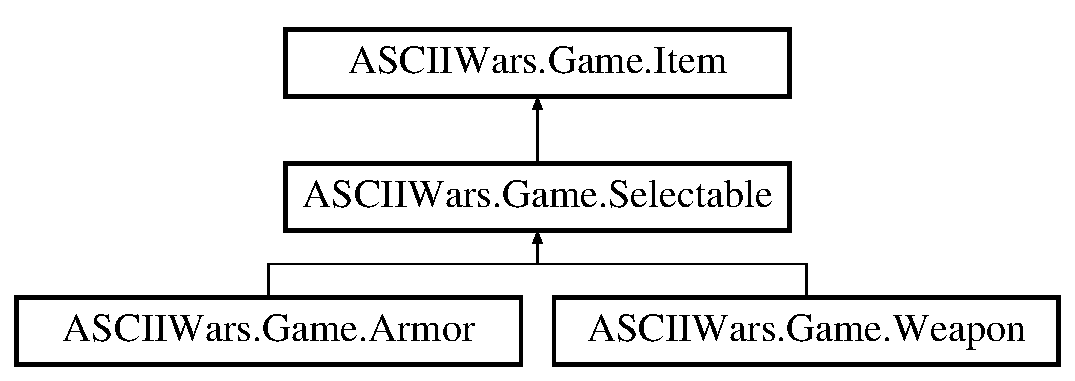
\includegraphics[height=3.000000cm]{class_a_s_c_i_i_wars_1_1_game_1_1_selectable}
\end{center}
\end{figure}
\subsection*{Открытые члены}
\begin{DoxyCompactItemize}
\item 
\hyperlink{class_a_s_c_i_i_wars_1_1_game_1_1_selectable_aa473dd0350842e4adfefa8e71accadd2}{Selectable} (string \hyperlink{class_a_s_c_i_i_wars_1_1_game_1_1_item_a744d51f7684a4e46a1f834f8666db58e}{id}, string \hyperlink{class_a_s_c_i_i_wars_1_1_game_1_1_item_a994b9ec5f10c123e4345da159c090091}{name}, string \hyperlink{class_a_s_c_i_i_wars_1_1_game_1_1_item_a6ff41e953ccebc64a8df8f8c434535a0}{description})
\item 
abstract void \hyperlink{class_a_s_c_i_i_wars_1_1_game_1_1_selectable_a95bdcf05ef9ea5f39c81ddd96294968a}{On\+Select\+By\+Player} (\hyperlink{class_a_s_c_i_i_wars_1_1_game_1_1_player}{Player} player)
\item 
abstract void \hyperlink{class_a_s_c_i_i_wars_1_1_game_1_1_selectable_a08a30c8786367bf45355e989b109c44b}{On\+Deselect\+By\+Player} (\hyperlink{class_a_s_c_i_i_wars_1_1_game_1_1_player}{Player} player)
\end{DoxyCompactItemize}
\subsection*{Открытые атрибуты}
\begin{DoxyCompactItemize}
\item 
bool \hyperlink{class_a_s_c_i_i_wars_1_1_game_1_1_selectable_ad864445e5408f11f74f2e5c843677fb2}{is\+Selected}
\end{DoxyCompactItemize}


\subsection{Конструктор(ы)}
\hypertarget{class_a_s_c_i_i_wars_1_1_game_1_1_selectable_aa473dd0350842e4adfefa8e71accadd2}{}\label{class_a_s_c_i_i_wars_1_1_game_1_1_selectable_aa473dd0350842e4adfefa8e71accadd2} 
\index{A\+S\+C\+I\+I\+Wars\+::\+Game\+::\+Selectable@{A\+S\+C\+I\+I\+Wars\+::\+Game\+::\+Selectable}!Selectable@{Selectable}}
\index{Selectable@{Selectable}!A\+S\+C\+I\+I\+Wars\+::\+Game\+::\+Selectable@{A\+S\+C\+I\+I\+Wars\+::\+Game\+::\+Selectable}}
\subsubsection{\texorpdfstring{Selectable()}{Selectable()}}
{\footnotesize\ttfamily A\+S\+C\+I\+I\+Wars.\+Game.\+Selectable.\+Selectable (\begin{DoxyParamCaption}\item[{string}]{id,  }\item[{string}]{name,  }\item[{string}]{description }\end{DoxyParamCaption})\hspace{0.3cm}{\ttfamily [inline]}}



\subsection{Методы}
\hypertarget{class_a_s_c_i_i_wars_1_1_game_1_1_selectable_a08a30c8786367bf45355e989b109c44b}{}\label{class_a_s_c_i_i_wars_1_1_game_1_1_selectable_a08a30c8786367bf45355e989b109c44b} 
\index{A\+S\+C\+I\+I\+Wars\+::\+Game\+::\+Selectable@{A\+S\+C\+I\+I\+Wars\+::\+Game\+::\+Selectable}!On\+Deselect\+By\+Player@{On\+Deselect\+By\+Player}}
\index{On\+Deselect\+By\+Player@{On\+Deselect\+By\+Player}!A\+S\+C\+I\+I\+Wars\+::\+Game\+::\+Selectable@{A\+S\+C\+I\+I\+Wars\+::\+Game\+::\+Selectable}}
\subsubsection{\texorpdfstring{On\+Deselect\+By\+Player()}{OnDeselectByPlayer()}}
{\footnotesize\ttfamily abstract void A\+S\+C\+I\+I\+Wars.\+Game.\+Selectable.\+On\+Deselect\+By\+Player (\begin{DoxyParamCaption}\item[{\hyperlink{class_a_s_c_i_i_wars_1_1_game_1_1_player}{Player}}]{player }\end{DoxyParamCaption})\hspace{0.3cm}{\ttfamily [pure virtual]}}



Замещается в \hyperlink{class_a_s_c_i_i_wars_1_1_game_1_1_armor_af502379d334f2fc7901638f8a8eba130}{A\+S\+C\+I\+I\+Wars.\+Game.\+Armor} и \hyperlink{class_a_s_c_i_i_wars_1_1_game_1_1_weapon_aa03a588bfb93fbf63d4d7bf63ce62ae1}{A\+S\+C\+I\+I\+Wars.\+Game.\+Weapon}.

\hypertarget{class_a_s_c_i_i_wars_1_1_game_1_1_selectable_a95bdcf05ef9ea5f39c81ddd96294968a}{}\label{class_a_s_c_i_i_wars_1_1_game_1_1_selectable_a95bdcf05ef9ea5f39c81ddd96294968a} 
\index{A\+S\+C\+I\+I\+Wars\+::\+Game\+::\+Selectable@{A\+S\+C\+I\+I\+Wars\+::\+Game\+::\+Selectable}!On\+Select\+By\+Player@{On\+Select\+By\+Player}}
\index{On\+Select\+By\+Player@{On\+Select\+By\+Player}!A\+S\+C\+I\+I\+Wars\+::\+Game\+::\+Selectable@{A\+S\+C\+I\+I\+Wars\+::\+Game\+::\+Selectable}}
\subsubsection{\texorpdfstring{On\+Select\+By\+Player()}{OnSelectByPlayer()}}
{\footnotesize\ttfamily abstract void A\+S\+C\+I\+I\+Wars.\+Game.\+Selectable.\+On\+Select\+By\+Player (\begin{DoxyParamCaption}\item[{\hyperlink{class_a_s_c_i_i_wars_1_1_game_1_1_player}{Player}}]{player }\end{DoxyParamCaption})\hspace{0.3cm}{\ttfamily [pure virtual]}}



Замещается в \hyperlink{class_a_s_c_i_i_wars_1_1_game_1_1_armor_ab4f8a39af009eef4bbdeb6db67fb9cd5}{A\+S\+C\+I\+I\+Wars.\+Game.\+Armor} и \hyperlink{class_a_s_c_i_i_wars_1_1_game_1_1_weapon_a6cd549ad51fa64884a66b1083098465f}{A\+S\+C\+I\+I\+Wars.\+Game.\+Weapon}.



\subsection{Данные класса}
\hypertarget{class_a_s_c_i_i_wars_1_1_game_1_1_selectable_ad864445e5408f11f74f2e5c843677fb2}{}\label{class_a_s_c_i_i_wars_1_1_game_1_1_selectable_ad864445e5408f11f74f2e5c843677fb2} 
\index{A\+S\+C\+I\+I\+Wars\+::\+Game\+::\+Selectable@{A\+S\+C\+I\+I\+Wars\+::\+Game\+::\+Selectable}!is\+Selected@{is\+Selected}}
\index{is\+Selected@{is\+Selected}!A\+S\+C\+I\+I\+Wars\+::\+Game\+::\+Selectable@{A\+S\+C\+I\+I\+Wars\+::\+Game\+::\+Selectable}}
\subsubsection{\texorpdfstring{is\+Selected}{isSelected}}
{\footnotesize\ttfamily bool A\+S\+C\+I\+I\+Wars.\+Game.\+Selectable.\+is\+Selected}



Объявления и описания членов класса находятся в файле\+:\begin{DoxyCompactItemize}
\item 
A\+S\+C\+I\+I\+Wars/\+Game/\hyperlink{_player_8cs}{Player.\+cs}\end{DoxyCompactItemize}

\hypertarget{class_a_s_c_i_i_wars_1_1_game_1_1_situation}{}\section{Класс A\+S\+C\+I\+I\+Wars.\+Game.\+Situation}
\label{class_a_s_c_i_i_wars_1_1_game_1_1_situation}\index{A\+S\+C\+I\+I\+Wars.\+Game.\+Situation@{A\+S\+C\+I\+I\+Wars.\+Game.\+Situation}}
\subsection*{Открытые атрибуты}
\begin{DoxyCompactItemize}
\item 
string \hyperlink{class_a_s_c_i_i_wars_1_1_game_1_1_situation_aefc60f917d443f47bdec48d9c45af5df}{type}
\item 
string \hyperlink{class_a_s_c_i_i_wars_1_1_game_1_1_situation_a84a39566fb7d8b3efa59e990597ac039}{object\+ID}
\end{DoxyCompactItemize}


\subsection{Данные класса}
\hypertarget{class_a_s_c_i_i_wars_1_1_game_1_1_situation_a84a39566fb7d8b3efa59e990597ac039}{}\label{class_a_s_c_i_i_wars_1_1_game_1_1_situation_a84a39566fb7d8b3efa59e990597ac039} 
\index{A\+S\+C\+I\+I\+Wars\+::\+Game\+::\+Situation@{A\+S\+C\+I\+I\+Wars\+::\+Game\+::\+Situation}!object\+ID@{object\+ID}}
\index{object\+ID@{object\+ID}!A\+S\+C\+I\+I\+Wars\+::\+Game\+::\+Situation@{A\+S\+C\+I\+I\+Wars\+::\+Game\+::\+Situation}}
\subsubsection{\texorpdfstring{object\+ID}{objectID}}
{\footnotesize\ttfamily string A\+S\+C\+I\+I\+Wars.\+Game.\+Situation.\+object\+ID}

\hypertarget{class_a_s_c_i_i_wars_1_1_game_1_1_situation_aefc60f917d443f47bdec48d9c45af5df}{}\label{class_a_s_c_i_i_wars_1_1_game_1_1_situation_aefc60f917d443f47bdec48d9c45af5df} 
\index{A\+S\+C\+I\+I\+Wars\+::\+Game\+::\+Situation@{A\+S\+C\+I\+I\+Wars\+::\+Game\+::\+Situation}!type@{type}}
\index{type@{type}!A\+S\+C\+I\+I\+Wars\+::\+Game\+::\+Situation@{A\+S\+C\+I\+I\+Wars\+::\+Game\+::\+Situation}}
\subsubsection{\texorpdfstring{type}{type}}
{\footnotesize\ttfamily string A\+S\+C\+I\+I\+Wars.\+Game.\+Situation.\+type}



Объявления и описания членов класса находятся в файле\+:\begin{DoxyCompactItemize}
\item 
A\+S\+C\+I\+I\+Wars/\+Game/\hyperlink{_situations_8cs}{Situations.\+cs}\end{DoxyCompactItemize}

\hypertarget{class_a_s_c_i_i_wars_1_1_game_1_1_situation_container}{}\section{Класс A\+S\+C\+I\+I\+Wars.\+Game.\+Situation\+Container}
\label{class_a_s_c_i_i_wars_1_1_game_1_1_situation_container}\index{A\+S\+C\+I\+I\+Wars.\+Game.\+Situation\+Container@{A\+S\+C\+I\+I\+Wars.\+Game.\+Situation\+Container}}
\subsection*{Открытые члены}
\begin{DoxyCompactItemize}
\item 
\hyperlink{class_a_s_c_i_i_wars_1_1_game_1_1_situation}{Situation} \hyperlink{class_a_s_c_i_i_wars_1_1_game_1_1_situation_container_a83ebb8c14380b5171524c8ebd4c2a581}{Random\+Situation\+By\+I\+Ds} (List$<$ string $>$ I\+Ds)
\item 
\hyperlink{class_a_s_c_i_i_wars_1_1_game_1_1_situation}{Situation} \hyperlink{class_a_s_c_i_i_wars_1_1_game_1_1_situation_container_aad379806144d48b5d6c66e409065473c}{Get\+Situation} (string id)
\item 
\hyperlink{class_a_s_c_i_i_wars_1_1_game_1_1_branch}{Branch} \hyperlink{class_a_s_c_i_i_wars_1_1_game_1_1_situation_container_a3bab9a3b20ced9a6b3408601ff381b51}{Get\+Branch} (string id)
\item 
\hyperlink{class_a_s_c_i_i_wars_1_1_game_1_1_enemy}{Enemy} \hyperlink{class_a_s_c_i_i_wars_1_1_game_1_1_situation_container_a559089971fe865f682768b43173181c4}{Get\+Enemy} (string id)
\item 
\hyperlink{class_a_s_c_i_i_wars_1_1_game_1_1_merchant}{Merchant} \hyperlink{class_a_s_c_i_i_wars_1_1_game_1_1_situation_container_a1e6b56a5e6db3eec1b59414956c245ae}{Get\+Merchant} (string id)
\item 
\hyperlink{class_a_s_c_i_i_wars_1_1_game_1_1_crafting_place}{Crafting\+Place} \hyperlink{class_a_s_c_i_i_wars_1_1_game_1_1_situation_container_a537f25cbf5d97a989954c421b6ea1a21}{Get\+Crafting\+Place} (string id)
\item 
\hyperlink{class_a_s_c_i_i_wars_1_1_game_1_1_quest}{Quest} \hyperlink{class_a_s_c_i_i_wars_1_1_game_1_1_situation_container_ac15145909b7206c2c2a7aa13f770a9a0}{Get\+Quest} (string id)
\end{DoxyCompactItemize}
\subsection*{Открытые атрибуты}
\begin{DoxyCompactItemize}
\item 
Dictionary$<$ string, \hyperlink{class_a_s_c_i_i_wars_1_1_game_1_1_situation}{Situation} $>$ \hyperlink{class_a_s_c_i_i_wars_1_1_game_1_1_situation_container_a24a982285b5782ecee43e98205d056c1}{situations}
\item 
Dictionary$<$ string, \hyperlink{class_a_s_c_i_i_wars_1_1_game_1_1_branch}{Branch} $>$ \hyperlink{class_a_s_c_i_i_wars_1_1_game_1_1_situation_container_af99ccf46ddcb93df3aa8ca830be1d2cd}{branches}
\item 
Dictionary$<$ string, \hyperlink{class_a_s_c_i_i_wars_1_1_game_1_1_enemy}{Enemy} $>$ \hyperlink{class_a_s_c_i_i_wars_1_1_game_1_1_situation_container_ae83c07e8b05da394daebe44f00e4f4d2}{enemies}
\item 
Dictionary$<$ string, \hyperlink{class_a_s_c_i_i_wars_1_1_game_1_1_merchant}{Merchant} $>$ \hyperlink{class_a_s_c_i_i_wars_1_1_game_1_1_situation_container_ad941813542c7012bd5867cc7962f1fee}{merchants}
\item 
Dictionary$<$ string, \hyperlink{class_a_s_c_i_i_wars_1_1_game_1_1_crafting_place}{Crafting\+Place} $>$ \hyperlink{class_a_s_c_i_i_wars_1_1_game_1_1_situation_container_a289c9b8afd2b2d3561f850e4ce6a4e0b}{crafting\+Places}
\item 
Dictionary$<$ string, \hyperlink{class_a_s_c_i_i_wars_1_1_game_1_1_quest}{Quest} $>$ \hyperlink{class_a_s_c_i_i_wars_1_1_game_1_1_situation_container_a1f019ada2eabbee7c5e51ecf9ce8d75a}{quests}
\end{DoxyCompactItemize}


\subsection{Методы}
\hypertarget{class_a_s_c_i_i_wars_1_1_game_1_1_situation_container_a3bab9a3b20ced9a6b3408601ff381b51}{}\label{class_a_s_c_i_i_wars_1_1_game_1_1_situation_container_a3bab9a3b20ced9a6b3408601ff381b51} 
\index{A\+S\+C\+I\+I\+Wars\+::\+Game\+::\+Situation\+Container@{A\+S\+C\+I\+I\+Wars\+::\+Game\+::\+Situation\+Container}!Get\+Branch@{Get\+Branch}}
\index{Get\+Branch@{Get\+Branch}!A\+S\+C\+I\+I\+Wars\+::\+Game\+::\+Situation\+Container@{A\+S\+C\+I\+I\+Wars\+::\+Game\+::\+Situation\+Container}}
\subsubsection{\texorpdfstring{Get\+Branch()}{GetBranch()}}
{\footnotesize\ttfamily \hyperlink{class_a_s_c_i_i_wars_1_1_game_1_1_branch}{Branch} A\+S\+C\+I\+I\+Wars.\+Game.\+Situation\+Container.\+Get\+Branch (\begin{DoxyParamCaption}\item[{string}]{id }\end{DoxyParamCaption})\hspace{0.3cm}{\ttfamily [inline]}}

\hypertarget{class_a_s_c_i_i_wars_1_1_game_1_1_situation_container_a537f25cbf5d97a989954c421b6ea1a21}{}\label{class_a_s_c_i_i_wars_1_1_game_1_1_situation_container_a537f25cbf5d97a989954c421b6ea1a21} 
\index{A\+S\+C\+I\+I\+Wars\+::\+Game\+::\+Situation\+Container@{A\+S\+C\+I\+I\+Wars\+::\+Game\+::\+Situation\+Container}!Get\+Crafting\+Place@{Get\+Crafting\+Place}}
\index{Get\+Crafting\+Place@{Get\+Crafting\+Place}!A\+S\+C\+I\+I\+Wars\+::\+Game\+::\+Situation\+Container@{A\+S\+C\+I\+I\+Wars\+::\+Game\+::\+Situation\+Container}}
\subsubsection{\texorpdfstring{Get\+Crafting\+Place()}{GetCraftingPlace()}}
{\footnotesize\ttfamily \hyperlink{class_a_s_c_i_i_wars_1_1_game_1_1_crafting_place}{Crafting\+Place} A\+S\+C\+I\+I\+Wars.\+Game.\+Situation\+Container.\+Get\+Crafting\+Place (\begin{DoxyParamCaption}\item[{string}]{id }\end{DoxyParamCaption})\hspace{0.3cm}{\ttfamily [inline]}}

\hypertarget{class_a_s_c_i_i_wars_1_1_game_1_1_situation_container_a559089971fe865f682768b43173181c4}{}\label{class_a_s_c_i_i_wars_1_1_game_1_1_situation_container_a559089971fe865f682768b43173181c4} 
\index{A\+S\+C\+I\+I\+Wars\+::\+Game\+::\+Situation\+Container@{A\+S\+C\+I\+I\+Wars\+::\+Game\+::\+Situation\+Container}!Get\+Enemy@{Get\+Enemy}}
\index{Get\+Enemy@{Get\+Enemy}!A\+S\+C\+I\+I\+Wars\+::\+Game\+::\+Situation\+Container@{A\+S\+C\+I\+I\+Wars\+::\+Game\+::\+Situation\+Container}}
\subsubsection{\texorpdfstring{Get\+Enemy()}{GetEnemy()}}
{\footnotesize\ttfamily \hyperlink{class_a_s_c_i_i_wars_1_1_game_1_1_enemy}{Enemy} A\+S\+C\+I\+I\+Wars.\+Game.\+Situation\+Container.\+Get\+Enemy (\begin{DoxyParamCaption}\item[{string}]{id }\end{DoxyParamCaption})\hspace{0.3cm}{\ttfamily [inline]}}

\hypertarget{class_a_s_c_i_i_wars_1_1_game_1_1_situation_container_a1e6b56a5e6db3eec1b59414956c245ae}{}\label{class_a_s_c_i_i_wars_1_1_game_1_1_situation_container_a1e6b56a5e6db3eec1b59414956c245ae} 
\index{A\+S\+C\+I\+I\+Wars\+::\+Game\+::\+Situation\+Container@{A\+S\+C\+I\+I\+Wars\+::\+Game\+::\+Situation\+Container}!Get\+Merchant@{Get\+Merchant}}
\index{Get\+Merchant@{Get\+Merchant}!A\+S\+C\+I\+I\+Wars\+::\+Game\+::\+Situation\+Container@{A\+S\+C\+I\+I\+Wars\+::\+Game\+::\+Situation\+Container}}
\subsubsection{\texorpdfstring{Get\+Merchant()}{GetMerchant()}}
{\footnotesize\ttfamily \hyperlink{class_a_s_c_i_i_wars_1_1_game_1_1_merchant}{Merchant} A\+S\+C\+I\+I\+Wars.\+Game.\+Situation\+Container.\+Get\+Merchant (\begin{DoxyParamCaption}\item[{string}]{id }\end{DoxyParamCaption})\hspace{0.3cm}{\ttfamily [inline]}}

\hypertarget{class_a_s_c_i_i_wars_1_1_game_1_1_situation_container_ac15145909b7206c2c2a7aa13f770a9a0}{}\label{class_a_s_c_i_i_wars_1_1_game_1_1_situation_container_ac15145909b7206c2c2a7aa13f770a9a0} 
\index{A\+S\+C\+I\+I\+Wars\+::\+Game\+::\+Situation\+Container@{A\+S\+C\+I\+I\+Wars\+::\+Game\+::\+Situation\+Container}!Get\+Quest@{Get\+Quest}}
\index{Get\+Quest@{Get\+Quest}!A\+S\+C\+I\+I\+Wars\+::\+Game\+::\+Situation\+Container@{A\+S\+C\+I\+I\+Wars\+::\+Game\+::\+Situation\+Container}}
\subsubsection{\texorpdfstring{Get\+Quest()}{GetQuest()}}
{\footnotesize\ttfamily \hyperlink{class_a_s_c_i_i_wars_1_1_game_1_1_quest}{Quest} A\+S\+C\+I\+I\+Wars.\+Game.\+Situation\+Container.\+Get\+Quest (\begin{DoxyParamCaption}\item[{string}]{id }\end{DoxyParamCaption})\hspace{0.3cm}{\ttfamily [inline]}}

\hypertarget{class_a_s_c_i_i_wars_1_1_game_1_1_situation_container_aad379806144d48b5d6c66e409065473c}{}\label{class_a_s_c_i_i_wars_1_1_game_1_1_situation_container_aad379806144d48b5d6c66e409065473c} 
\index{A\+S\+C\+I\+I\+Wars\+::\+Game\+::\+Situation\+Container@{A\+S\+C\+I\+I\+Wars\+::\+Game\+::\+Situation\+Container}!Get\+Situation@{Get\+Situation}}
\index{Get\+Situation@{Get\+Situation}!A\+S\+C\+I\+I\+Wars\+::\+Game\+::\+Situation\+Container@{A\+S\+C\+I\+I\+Wars\+::\+Game\+::\+Situation\+Container}}
\subsubsection{\texorpdfstring{Get\+Situation()}{GetSituation()}}
{\footnotesize\ttfamily \hyperlink{class_a_s_c_i_i_wars_1_1_game_1_1_situation}{Situation} A\+S\+C\+I\+I\+Wars.\+Game.\+Situation\+Container.\+Get\+Situation (\begin{DoxyParamCaption}\item[{string}]{id }\end{DoxyParamCaption})\hspace{0.3cm}{\ttfamily [inline]}}

\hypertarget{class_a_s_c_i_i_wars_1_1_game_1_1_situation_container_a83ebb8c14380b5171524c8ebd4c2a581}{}\label{class_a_s_c_i_i_wars_1_1_game_1_1_situation_container_a83ebb8c14380b5171524c8ebd4c2a581} 
\index{A\+S\+C\+I\+I\+Wars\+::\+Game\+::\+Situation\+Container@{A\+S\+C\+I\+I\+Wars\+::\+Game\+::\+Situation\+Container}!Random\+Situation\+By\+I\+Ds@{Random\+Situation\+By\+I\+Ds}}
\index{Random\+Situation\+By\+I\+Ds@{Random\+Situation\+By\+I\+Ds}!A\+S\+C\+I\+I\+Wars\+::\+Game\+::\+Situation\+Container@{A\+S\+C\+I\+I\+Wars\+::\+Game\+::\+Situation\+Container}}
\subsubsection{\texorpdfstring{Random\+Situation\+By\+I\+Ds()}{RandomSituationByIDs()}}
{\footnotesize\ttfamily \hyperlink{class_a_s_c_i_i_wars_1_1_game_1_1_situation}{Situation} A\+S\+C\+I\+I\+Wars.\+Game.\+Situation\+Container.\+Random\+Situation\+By\+I\+Ds (\begin{DoxyParamCaption}\item[{List$<$ string $>$}]{I\+Ds }\end{DoxyParamCaption})\hspace{0.3cm}{\ttfamily [inline]}}



\subsection{Данные класса}
\hypertarget{class_a_s_c_i_i_wars_1_1_game_1_1_situation_container_af99ccf46ddcb93df3aa8ca830be1d2cd}{}\label{class_a_s_c_i_i_wars_1_1_game_1_1_situation_container_af99ccf46ddcb93df3aa8ca830be1d2cd} 
\index{A\+S\+C\+I\+I\+Wars\+::\+Game\+::\+Situation\+Container@{A\+S\+C\+I\+I\+Wars\+::\+Game\+::\+Situation\+Container}!branches@{branches}}
\index{branches@{branches}!A\+S\+C\+I\+I\+Wars\+::\+Game\+::\+Situation\+Container@{A\+S\+C\+I\+I\+Wars\+::\+Game\+::\+Situation\+Container}}
\subsubsection{\texorpdfstring{branches}{branches}}
{\footnotesize\ttfamily Dictionary$<$string, \hyperlink{class_a_s_c_i_i_wars_1_1_game_1_1_branch}{Branch}$>$ A\+S\+C\+I\+I\+Wars.\+Game.\+Situation\+Container.\+branches}

\hypertarget{class_a_s_c_i_i_wars_1_1_game_1_1_situation_container_a289c9b8afd2b2d3561f850e4ce6a4e0b}{}\label{class_a_s_c_i_i_wars_1_1_game_1_1_situation_container_a289c9b8afd2b2d3561f850e4ce6a4e0b} 
\index{A\+S\+C\+I\+I\+Wars\+::\+Game\+::\+Situation\+Container@{A\+S\+C\+I\+I\+Wars\+::\+Game\+::\+Situation\+Container}!crafting\+Places@{crafting\+Places}}
\index{crafting\+Places@{crafting\+Places}!A\+S\+C\+I\+I\+Wars\+::\+Game\+::\+Situation\+Container@{A\+S\+C\+I\+I\+Wars\+::\+Game\+::\+Situation\+Container}}
\subsubsection{\texorpdfstring{crafting\+Places}{craftingPlaces}}
{\footnotesize\ttfamily Dictionary$<$string, \hyperlink{class_a_s_c_i_i_wars_1_1_game_1_1_crafting_place}{Crafting\+Place}$>$ A\+S\+C\+I\+I\+Wars.\+Game.\+Situation\+Container.\+crafting\+Places}

\hypertarget{class_a_s_c_i_i_wars_1_1_game_1_1_situation_container_ae83c07e8b05da394daebe44f00e4f4d2}{}\label{class_a_s_c_i_i_wars_1_1_game_1_1_situation_container_ae83c07e8b05da394daebe44f00e4f4d2} 
\index{A\+S\+C\+I\+I\+Wars\+::\+Game\+::\+Situation\+Container@{A\+S\+C\+I\+I\+Wars\+::\+Game\+::\+Situation\+Container}!enemies@{enemies}}
\index{enemies@{enemies}!A\+S\+C\+I\+I\+Wars\+::\+Game\+::\+Situation\+Container@{A\+S\+C\+I\+I\+Wars\+::\+Game\+::\+Situation\+Container}}
\subsubsection{\texorpdfstring{enemies}{enemies}}
{\footnotesize\ttfamily Dictionary$<$string, \hyperlink{class_a_s_c_i_i_wars_1_1_game_1_1_enemy}{Enemy}$>$ A\+S\+C\+I\+I\+Wars.\+Game.\+Situation\+Container.\+enemies}

\hypertarget{class_a_s_c_i_i_wars_1_1_game_1_1_situation_container_ad941813542c7012bd5867cc7962f1fee}{}\label{class_a_s_c_i_i_wars_1_1_game_1_1_situation_container_ad941813542c7012bd5867cc7962f1fee} 
\index{A\+S\+C\+I\+I\+Wars\+::\+Game\+::\+Situation\+Container@{A\+S\+C\+I\+I\+Wars\+::\+Game\+::\+Situation\+Container}!merchants@{merchants}}
\index{merchants@{merchants}!A\+S\+C\+I\+I\+Wars\+::\+Game\+::\+Situation\+Container@{A\+S\+C\+I\+I\+Wars\+::\+Game\+::\+Situation\+Container}}
\subsubsection{\texorpdfstring{merchants}{merchants}}
{\footnotesize\ttfamily Dictionary$<$string, \hyperlink{class_a_s_c_i_i_wars_1_1_game_1_1_merchant}{Merchant}$>$ A\+S\+C\+I\+I\+Wars.\+Game.\+Situation\+Container.\+merchants}

\hypertarget{class_a_s_c_i_i_wars_1_1_game_1_1_situation_container_a1f019ada2eabbee7c5e51ecf9ce8d75a}{}\label{class_a_s_c_i_i_wars_1_1_game_1_1_situation_container_a1f019ada2eabbee7c5e51ecf9ce8d75a} 
\index{A\+S\+C\+I\+I\+Wars\+::\+Game\+::\+Situation\+Container@{A\+S\+C\+I\+I\+Wars\+::\+Game\+::\+Situation\+Container}!quests@{quests}}
\index{quests@{quests}!A\+S\+C\+I\+I\+Wars\+::\+Game\+::\+Situation\+Container@{A\+S\+C\+I\+I\+Wars\+::\+Game\+::\+Situation\+Container}}
\subsubsection{\texorpdfstring{quests}{quests}}
{\footnotesize\ttfamily Dictionary$<$string, \hyperlink{class_a_s_c_i_i_wars_1_1_game_1_1_quest}{Quest}$>$ A\+S\+C\+I\+I\+Wars.\+Game.\+Situation\+Container.\+quests}

\hypertarget{class_a_s_c_i_i_wars_1_1_game_1_1_situation_container_a24a982285b5782ecee43e98205d056c1}{}\label{class_a_s_c_i_i_wars_1_1_game_1_1_situation_container_a24a982285b5782ecee43e98205d056c1} 
\index{A\+S\+C\+I\+I\+Wars\+::\+Game\+::\+Situation\+Container@{A\+S\+C\+I\+I\+Wars\+::\+Game\+::\+Situation\+Container}!situations@{situations}}
\index{situations@{situations}!A\+S\+C\+I\+I\+Wars\+::\+Game\+::\+Situation\+Container@{A\+S\+C\+I\+I\+Wars\+::\+Game\+::\+Situation\+Container}}
\subsubsection{\texorpdfstring{situations}{situations}}
{\footnotesize\ttfamily Dictionary$<$string, \hyperlink{class_a_s_c_i_i_wars_1_1_game_1_1_situation}{Situation}$>$ A\+S\+C\+I\+I\+Wars.\+Game.\+Situation\+Container.\+situations}



Объявления и описания членов класса находятся в файле\+:\begin{DoxyCompactItemize}
\item 
A\+S\+C\+I\+I\+Wars/\+Game/\hyperlink{_situations_8cs}{Situations.\+cs}\end{DoxyCompactItemize}

\hypertarget{class_a_s_c_i_i_wars_1_1_console_graphics_1_1_task}{}\section{Класс A\+S\+C\+I\+I\+Wars.\+Console\+Graphics.\+Task}
\label{class_a_s_c_i_i_wars_1_1_console_graphics_1_1_task}\index{A\+S\+C\+I\+I\+Wars.\+Console\+Graphics.\+Task@{A\+S\+C\+I\+I\+Wars.\+Console\+Graphics.\+Task}}
\subsection*{Открытые члены}
\begin{DoxyCompactItemize}
\item 
\hyperlink{class_a_s_c_i_i_wars_1_1_console_graphics_1_1_task_a2fe2e33110134ec07ed7ad5960976c6a}{Task} (string \hyperlink{class_a_s_c_i_i_wars_1_1_console_graphics_1_1_task_a235e892a10d43807b743c0edf8855df3}{name}, Action \hyperlink{class_a_s_c_i_i_wars_1_1_console_graphics_1_1_task_a9fcf12d48e7ae10b20db0828cedf4f7d}{action})
\item 
\hyperlink{class_a_s_c_i_i_wars_1_1_console_graphics_1_1_task_a083e89927241325952a8790824b79f83}{Task} (Func$<$ string $>$ \hyperlink{class_a_s_c_i_i_wars_1_1_console_graphics_1_1_task_ad5fe90ee93b95cf0be9ec7d6d533dabc}{name\+Supplier}, Action \hyperlink{class_a_s_c_i_i_wars_1_1_console_graphics_1_1_task_a9fcf12d48e7ae10b20db0828cedf4f7d}{action})
\end{DoxyCompactItemize}
\subsection*{Открытые статические члены}
\begin{DoxyCompactItemize}
\item 
static \hyperlink{class_a_s_c_i_i_wars_1_1_console_graphics_1_1_task}{Task} \hyperlink{class_a_s_c_i_i_wars_1_1_console_graphics_1_1_task_a199974d73498b9de5c95c3e90864a59b}{Empty\+Task} (string \hyperlink{class_a_s_c_i_i_wars_1_1_console_graphics_1_1_task_a235e892a10d43807b743c0edf8855df3}{name}, int delay)
\end{DoxyCompactItemize}
\subsection*{Открытые атрибуты}
\begin{DoxyCompactItemize}
\item 
readonly Func$<$ string $>$ \hyperlink{class_a_s_c_i_i_wars_1_1_console_graphics_1_1_task_ad5fe90ee93b95cf0be9ec7d6d533dabc}{name\+Supplier}
\item 
readonly Action \hyperlink{class_a_s_c_i_i_wars_1_1_console_graphics_1_1_task_a9fcf12d48e7ae10b20db0828cedf4f7d}{action}
\end{DoxyCompactItemize}
\subsection*{Свойства}
\begin{DoxyCompactItemize}
\item 
string \hyperlink{class_a_s_c_i_i_wars_1_1_console_graphics_1_1_task_a235e892a10d43807b743c0edf8855df3}{name}\hspace{0.3cm}{\ttfamily  \mbox{[}get\mbox{]}}
\end{DoxyCompactItemize}


\subsection{Конструктор(ы)}
\hypertarget{class_a_s_c_i_i_wars_1_1_console_graphics_1_1_task_a2fe2e33110134ec07ed7ad5960976c6a}{}\label{class_a_s_c_i_i_wars_1_1_console_graphics_1_1_task_a2fe2e33110134ec07ed7ad5960976c6a} 
\index{A\+S\+C\+I\+I\+Wars\+::\+Console\+Graphics\+::\+Task@{A\+S\+C\+I\+I\+Wars\+::\+Console\+Graphics\+::\+Task}!Task@{Task}}
\index{Task@{Task}!A\+S\+C\+I\+I\+Wars\+::\+Console\+Graphics\+::\+Task@{A\+S\+C\+I\+I\+Wars\+::\+Console\+Graphics\+::\+Task}}
\subsubsection{\texorpdfstring{Task()}{Task()}\hspace{0.1cm}{\footnotesize\ttfamily [1/2]}}
{\footnotesize\ttfamily A\+S\+C\+I\+I\+Wars.\+Console\+Graphics.\+Task.\+Task (\begin{DoxyParamCaption}\item[{string}]{name,  }\item[{Action}]{action }\end{DoxyParamCaption})\hspace{0.3cm}{\ttfamily [inline]}}

\hypertarget{class_a_s_c_i_i_wars_1_1_console_graphics_1_1_task_a083e89927241325952a8790824b79f83}{}\label{class_a_s_c_i_i_wars_1_1_console_graphics_1_1_task_a083e89927241325952a8790824b79f83} 
\index{A\+S\+C\+I\+I\+Wars\+::\+Console\+Graphics\+::\+Task@{A\+S\+C\+I\+I\+Wars\+::\+Console\+Graphics\+::\+Task}!Task@{Task}}
\index{Task@{Task}!A\+S\+C\+I\+I\+Wars\+::\+Console\+Graphics\+::\+Task@{A\+S\+C\+I\+I\+Wars\+::\+Console\+Graphics\+::\+Task}}
\subsubsection{\texorpdfstring{Task()}{Task()}\hspace{0.1cm}{\footnotesize\ttfamily [2/2]}}
{\footnotesize\ttfamily A\+S\+C\+I\+I\+Wars.\+Console\+Graphics.\+Task.\+Task (\begin{DoxyParamCaption}\item[{Func$<$ string $>$}]{name\+Supplier,  }\item[{Action}]{action }\end{DoxyParamCaption})\hspace{0.3cm}{\ttfamily [inline]}}



\subsection{Методы}
\hypertarget{class_a_s_c_i_i_wars_1_1_console_graphics_1_1_task_a199974d73498b9de5c95c3e90864a59b}{}\label{class_a_s_c_i_i_wars_1_1_console_graphics_1_1_task_a199974d73498b9de5c95c3e90864a59b} 
\index{A\+S\+C\+I\+I\+Wars\+::\+Console\+Graphics\+::\+Task@{A\+S\+C\+I\+I\+Wars\+::\+Console\+Graphics\+::\+Task}!Empty\+Task@{Empty\+Task}}
\index{Empty\+Task@{Empty\+Task}!A\+S\+C\+I\+I\+Wars\+::\+Console\+Graphics\+::\+Task@{A\+S\+C\+I\+I\+Wars\+::\+Console\+Graphics\+::\+Task}}
\subsubsection{\texorpdfstring{Empty\+Task()}{EmptyTask()}}
{\footnotesize\ttfamily static \hyperlink{class_a_s_c_i_i_wars_1_1_console_graphics_1_1_task}{Task} A\+S\+C\+I\+I\+Wars.\+Console\+Graphics.\+Task.\+Empty\+Task (\begin{DoxyParamCaption}\item[{string}]{name,  }\item[{int}]{delay }\end{DoxyParamCaption})\hspace{0.3cm}{\ttfamily [inline]}, {\ttfamily [static]}}



\subsection{Данные класса}
\hypertarget{class_a_s_c_i_i_wars_1_1_console_graphics_1_1_task_a9fcf12d48e7ae10b20db0828cedf4f7d}{}\label{class_a_s_c_i_i_wars_1_1_console_graphics_1_1_task_a9fcf12d48e7ae10b20db0828cedf4f7d} 
\index{A\+S\+C\+I\+I\+Wars\+::\+Console\+Graphics\+::\+Task@{A\+S\+C\+I\+I\+Wars\+::\+Console\+Graphics\+::\+Task}!action@{action}}
\index{action@{action}!A\+S\+C\+I\+I\+Wars\+::\+Console\+Graphics\+::\+Task@{A\+S\+C\+I\+I\+Wars\+::\+Console\+Graphics\+::\+Task}}
\subsubsection{\texorpdfstring{action}{action}}
{\footnotesize\ttfamily readonly Action A\+S\+C\+I\+I\+Wars.\+Console\+Graphics.\+Task.\+action}

\hypertarget{class_a_s_c_i_i_wars_1_1_console_graphics_1_1_task_ad5fe90ee93b95cf0be9ec7d6d533dabc}{}\label{class_a_s_c_i_i_wars_1_1_console_graphics_1_1_task_ad5fe90ee93b95cf0be9ec7d6d533dabc} 
\index{A\+S\+C\+I\+I\+Wars\+::\+Console\+Graphics\+::\+Task@{A\+S\+C\+I\+I\+Wars\+::\+Console\+Graphics\+::\+Task}!name\+Supplier@{name\+Supplier}}
\index{name\+Supplier@{name\+Supplier}!A\+S\+C\+I\+I\+Wars\+::\+Console\+Graphics\+::\+Task@{A\+S\+C\+I\+I\+Wars\+::\+Console\+Graphics\+::\+Task}}
\subsubsection{\texorpdfstring{name\+Supplier}{nameSupplier}}
{\footnotesize\ttfamily readonly Func$<$string$>$ A\+S\+C\+I\+I\+Wars.\+Console\+Graphics.\+Task.\+name\+Supplier}



\subsection{Полный список свойств}
\hypertarget{class_a_s_c_i_i_wars_1_1_console_graphics_1_1_task_a235e892a10d43807b743c0edf8855df3}{}\label{class_a_s_c_i_i_wars_1_1_console_graphics_1_1_task_a235e892a10d43807b743c0edf8855df3} 
\index{A\+S\+C\+I\+I\+Wars\+::\+Console\+Graphics\+::\+Task@{A\+S\+C\+I\+I\+Wars\+::\+Console\+Graphics\+::\+Task}!name@{name}}
\index{name@{name}!A\+S\+C\+I\+I\+Wars\+::\+Console\+Graphics\+::\+Task@{A\+S\+C\+I\+I\+Wars\+::\+Console\+Graphics\+::\+Task}}
\subsubsection{\texorpdfstring{name}{name}}
{\footnotesize\ttfamily string A\+S\+C\+I\+I\+Wars.\+Console\+Graphics.\+Task.\+name\hspace{0.3cm}{\ttfamily [get]}}



Объявления и описания членов класса находятся в файле\+:\begin{DoxyCompactItemize}
\item 
Console\+Graphics/\hyperlink{_loading_bar_8cs}{Loading\+Bar.\+cs}\end{DoxyCompactItemize}

\hypertarget{class_a_s_c_i_i_wars_1_1_game_1_1_weapon}{}\section{Класс A\+S\+C\+I\+I\+Wars.\+Game.\+Weapon}
\label{class_a_s_c_i_i_wars_1_1_game_1_1_weapon}\index{A\+S\+C\+I\+I\+Wars.\+Game.\+Weapon@{A\+S\+C\+I\+I\+Wars.\+Game.\+Weapon}}
Граф наследования\+:A\+S\+C\+I\+I\+Wars.\+Game.\+Weapon\+:\begin{figure}[H]
\begin{center}
\leavevmode
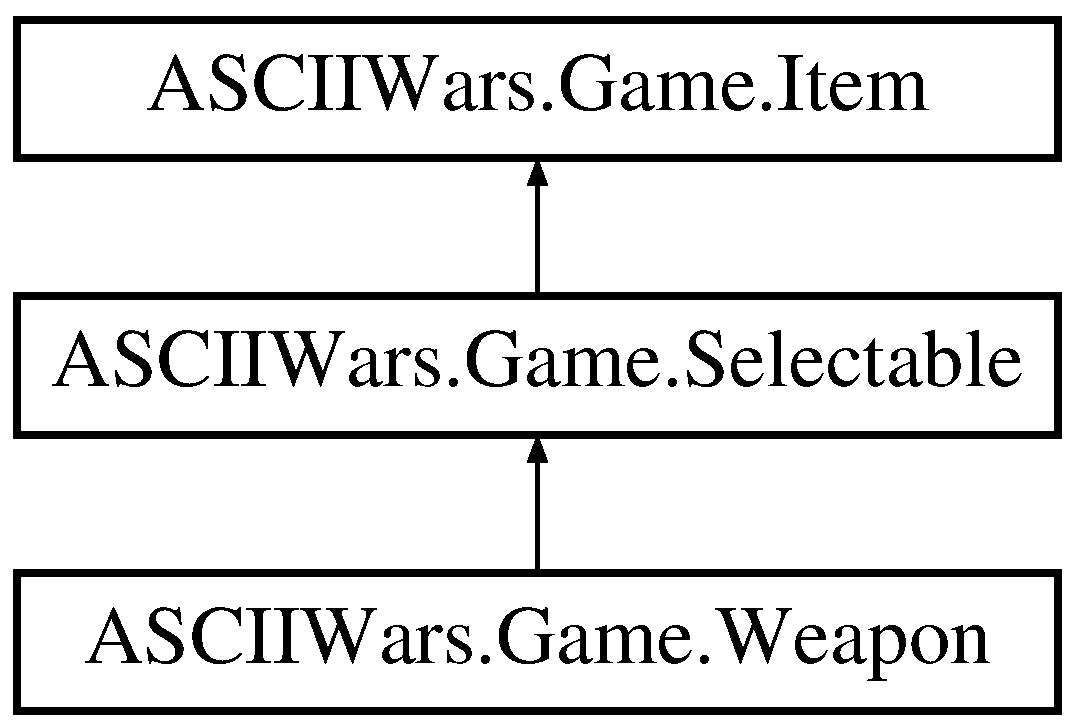
\includegraphics[height=3.000000cm]{class_a_s_c_i_i_wars_1_1_game_1_1_weapon}
\end{center}
\end{figure}
\subsection*{Открытые члены}
\begin{DoxyCompactItemize}
\item 
\hyperlink{class_a_s_c_i_i_wars_1_1_game_1_1_weapon_ab292fb175c5d6e29ec2918069f831d4c}{Weapon} (string \hyperlink{class_a_s_c_i_i_wars_1_1_game_1_1_item_a744d51f7684a4e46a1f834f8666db58e}{id}, string \hyperlink{class_a_s_c_i_i_wars_1_1_game_1_1_item_a994b9ec5f10c123e4345da159c090091}{name}, string \hyperlink{class_a_s_c_i_i_wars_1_1_game_1_1_item_a6ff41e953ccebc64a8df8f8c434535a0}{description}, int \hyperlink{class_a_s_c_i_i_wars_1_1_game_1_1_weapon_a70166ce84757794de92f0a52de55bb04}{attack})
\item 
override void \hyperlink{class_a_s_c_i_i_wars_1_1_game_1_1_weapon_ad29135a3edb4ea03f29163d788364299}{On\+Add\+To\+Player\+Inventory} (\hyperlink{class_a_s_c_i_i_wars_1_1_game_1_1_player}{Player} player)
\item 
override void \hyperlink{class_a_s_c_i_i_wars_1_1_game_1_1_weapon_a6cd549ad51fa64884a66b1083098465f}{On\+Select\+By\+Player} (\hyperlink{class_a_s_c_i_i_wars_1_1_game_1_1_player}{Player} player)
\item 
override void \hyperlink{class_a_s_c_i_i_wars_1_1_game_1_1_weapon_aa03a588bfb93fbf63d4d7bf63ce62ae1}{On\+Deselect\+By\+Player} (\hyperlink{class_a_s_c_i_i_wars_1_1_game_1_1_player}{Player} player)
\item 
override void \hyperlink{class_a_s_c_i_i_wars_1_1_game_1_1_weapon_a1fc9edec1d3881aee188a30ddc8f9e58}{On\+Remove\+From\+Player\+Inventory} (\hyperlink{class_a_s_c_i_i_wars_1_1_game_1_1_player}{Player} player)
\item 
override int \hyperlink{class_a_s_c_i_i_wars_1_1_game_1_1_weapon_af252081d5a5f047785ed545946bb5214}{Get\+Hash\+Code} ()
\item 
override bool \hyperlink{class_a_s_c_i_i_wars_1_1_game_1_1_weapon_a281a4ca4d8a376aeda8408551ee168cf}{Equals} (object obj)
\end{DoxyCompactItemize}
\subsection*{Открытые атрибуты}
\begin{DoxyCompactItemize}
\item 
readonly int \hyperlink{class_a_s_c_i_i_wars_1_1_game_1_1_weapon_a70166ce84757794de92f0a52de55bb04}{attack}
\end{DoxyCompactItemize}


\subsection{Конструктор(ы)}
\hypertarget{class_a_s_c_i_i_wars_1_1_game_1_1_weapon_ab292fb175c5d6e29ec2918069f831d4c}{}\label{class_a_s_c_i_i_wars_1_1_game_1_1_weapon_ab292fb175c5d6e29ec2918069f831d4c} 
\index{A\+S\+C\+I\+I\+Wars\+::\+Game\+::\+Weapon@{A\+S\+C\+I\+I\+Wars\+::\+Game\+::\+Weapon}!Weapon@{Weapon}}
\index{Weapon@{Weapon}!A\+S\+C\+I\+I\+Wars\+::\+Game\+::\+Weapon@{A\+S\+C\+I\+I\+Wars\+::\+Game\+::\+Weapon}}
\subsubsection{\texorpdfstring{Weapon()}{Weapon()}}
{\footnotesize\ttfamily A\+S\+C\+I\+I\+Wars.\+Game.\+Weapon.\+Weapon (\begin{DoxyParamCaption}\item[{string}]{id,  }\item[{string}]{name,  }\item[{string}]{description,  }\item[{int}]{attack }\end{DoxyParamCaption})\hspace{0.3cm}{\ttfamily [inline]}}



\subsection{Методы}
\hypertarget{class_a_s_c_i_i_wars_1_1_game_1_1_weapon_a281a4ca4d8a376aeda8408551ee168cf}{}\label{class_a_s_c_i_i_wars_1_1_game_1_1_weapon_a281a4ca4d8a376aeda8408551ee168cf} 
\index{A\+S\+C\+I\+I\+Wars\+::\+Game\+::\+Weapon@{A\+S\+C\+I\+I\+Wars\+::\+Game\+::\+Weapon}!Equals@{Equals}}
\index{Equals@{Equals}!A\+S\+C\+I\+I\+Wars\+::\+Game\+::\+Weapon@{A\+S\+C\+I\+I\+Wars\+::\+Game\+::\+Weapon}}
\subsubsection{\texorpdfstring{Equals()}{Equals()}}
{\footnotesize\ttfamily override bool A\+S\+C\+I\+I\+Wars.\+Game.\+Weapon.\+Equals (\begin{DoxyParamCaption}\item[{object}]{obj }\end{DoxyParamCaption})\hspace{0.3cm}{\ttfamily [inline]}}

\hypertarget{class_a_s_c_i_i_wars_1_1_game_1_1_weapon_af252081d5a5f047785ed545946bb5214}{}\label{class_a_s_c_i_i_wars_1_1_game_1_1_weapon_af252081d5a5f047785ed545946bb5214} 
\index{A\+S\+C\+I\+I\+Wars\+::\+Game\+::\+Weapon@{A\+S\+C\+I\+I\+Wars\+::\+Game\+::\+Weapon}!Get\+Hash\+Code@{Get\+Hash\+Code}}
\index{Get\+Hash\+Code@{Get\+Hash\+Code}!A\+S\+C\+I\+I\+Wars\+::\+Game\+::\+Weapon@{A\+S\+C\+I\+I\+Wars\+::\+Game\+::\+Weapon}}
\subsubsection{\texorpdfstring{Get\+Hash\+Code()}{GetHashCode()}}
{\footnotesize\ttfamily override int A\+S\+C\+I\+I\+Wars.\+Game.\+Weapon.\+Get\+Hash\+Code (\begin{DoxyParamCaption}{ }\end{DoxyParamCaption})\hspace{0.3cm}{\ttfamily [inline]}}

\hypertarget{class_a_s_c_i_i_wars_1_1_game_1_1_weapon_ad29135a3edb4ea03f29163d788364299}{}\label{class_a_s_c_i_i_wars_1_1_game_1_1_weapon_ad29135a3edb4ea03f29163d788364299} 
\index{A\+S\+C\+I\+I\+Wars\+::\+Game\+::\+Weapon@{A\+S\+C\+I\+I\+Wars\+::\+Game\+::\+Weapon}!On\+Add\+To\+Player\+Inventory@{On\+Add\+To\+Player\+Inventory}}
\index{On\+Add\+To\+Player\+Inventory@{On\+Add\+To\+Player\+Inventory}!A\+S\+C\+I\+I\+Wars\+::\+Game\+::\+Weapon@{A\+S\+C\+I\+I\+Wars\+::\+Game\+::\+Weapon}}
\subsubsection{\texorpdfstring{On\+Add\+To\+Player\+Inventory()}{OnAddToPlayerInventory()}}
{\footnotesize\ttfamily override void A\+S\+C\+I\+I\+Wars.\+Game.\+Weapon.\+On\+Add\+To\+Player\+Inventory (\begin{DoxyParamCaption}\item[{\hyperlink{class_a_s_c_i_i_wars_1_1_game_1_1_player}{Player}}]{player }\end{DoxyParamCaption})\hspace{0.3cm}{\ttfamily [inline]}, {\ttfamily [virtual]}}



Замещает \hyperlink{class_a_s_c_i_i_wars_1_1_game_1_1_item_aec0355b7a9f647ef24897b95563f70d1}{A\+S\+C\+I\+I\+Wars.\+Game.\+Item}.

\hypertarget{class_a_s_c_i_i_wars_1_1_game_1_1_weapon_aa03a588bfb93fbf63d4d7bf63ce62ae1}{}\label{class_a_s_c_i_i_wars_1_1_game_1_1_weapon_aa03a588bfb93fbf63d4d7bf63ce62ae1} 
\index{A\+S\+C\+I\+I\+Wars\+::\+Game\+::\+Weapon@{A\+S\+C\+I\+I\+Wars\+::\+Game\+::\+Weapon}!On\+Deselect\+By\+Player@{On\+Deselect\+By\+Player}}
\index{On\+Deselect\+By\+Player@{On\+Deselect\+By\+Player}!A\+S\+C\+I\+I\+Wars\+::\+Game\+::\+Weapon@{A\+S\+C\+I\+I\+Wars\+::\+Game\+::\+Weapon}}
\subsubsection{\texorpdfstring{On\+Deselect\+By\+Player()}{OnDeselectByPlayer()}}
{\footnotesize\ttfamily override void A\+S\+C\+I\+I\+Wars.\+Game.\+Weapon.\+On\+Deselect\+By\+Player (\begin{DoxyParamCaption}\item[{\hyperlink{class_a_s_c_i_i_wars_1_1_game_1_1_player}{Player}}]{player }\end{DoxyParamCaption})\hspace{0.3cm}{\ttfamily [inline]}, {\ttfamily [virtual]}}



Замещает \hyperlink{class_a_s_c_i_i_wars_1_1_game_1_1_selectable_a08a30c8786367bf45355e989b109c44b}{A\+S\+C\+I\+I\+Wars.\+Game.\+Selectable}.

\hypertarget{class_a_s_c_i_i_wars_1_1_game_1_1_weapon_a1fc9edec1d3881aee188a30ddc8f9e58}{}\label{class_a_s_c_i_i_wars_1_1_game_1_1_weapon_a1fc9edec1d3881aee188a30ddc8f9e58} 
\index{A\+S\+C\+I\+I\+Wars\+::\+Game\+::\+Weapon@{A\+S\+C\+I\+I\+Wars\+::\+Game\+::\+Weapon}!On\+Remove\+From\+Player\+Inventory@{On\+Remove\+From\+Player\+Inventory}}
\index{On\+Remove\+From\+Player\+Inventory@{On\+Remove\+From\+Player\+Inventory}!A\+S\+C\+I\+I\+Wars\+::\+Game\+::\+Weapon@{A\+S\+C\+I\+I\+Wars\+::\+Game\+::\+Weapon}}
\subsubsection{\texorpdfstring{On\+Remove\+From\+Player\+Inventory()}{OnRemoveFromPlayerInventory()}}
{\footnotesize\ttfamily override void A\+S\+C\+I\+I\+Wars.\+Game.\+Weapon.\+On\+Remove\+From\+Player\+Inventory (\begin{DoxyParamCaption}\item[{\hyperlink{class_a_s_c_i_i_wars_1_1_game_1_1_player}{Player}}]{player }\end{DoxyParamCaption})\hspace{0.3cm}{\ttfamily [inline]}, {\ttfamily [virtual]}}



Замещает \hyperlink{class_a_s_c_i_i_wars_1_1_game_1_1_item_a52412546f837bfc65a3aa9d728fa142f}{A\+S\+C\+I\+I\+Wars.\+Game.\+Item}.

\hypertarget{class_a_s_c_i_i_wars_1_1_game_1_1_weapon_a6cd549ad51fa64884a66b1083098465f}{}\label{class_a_s_c_i_i_wars_1_1_game_1_1_weapon_a6cd549ad51fa64884a66b1083098465f} 
\index{A\+S\+C\+I\+I\+Wars\+::\+Game\+::\+Weapon@{A\+S\+C\+I\+I\+Wars\+::\+Game\+::\+Weapon}!On\+Select\+By\+Player@{On\+Select\+By\+Player}}
\index{On\+Select\+By\+Player@{On\+Select\+By\+Player}!A\+S\+C\+I\+I\+Wars\+::\+Game\+::\+Weapon@{A\+S\+C\+I\+I\+Wars\+::\+Game\+::\+Weapon}}
\subsubsection{\texorpdfstring{On\+Select\+By\+Player()}{OnSelectByPlayer()}}
{\footnotesize\ttfamily override void A\+S\+C\+I\+I\+Wars.\+Game.\+Weapon.\+On\+Select\+By\+Player (\begin{DoxyParamCaption}\item[{\hyperlink{class_a_s_c_i_i_wars_1_1_game_1_1_player}{Player}}]{player }\end{DoxyParamCaption})\hspace{0.3cm}{\ttfamily [inline]}, {\ttfamily [virtual]}}



Замещает \hyperlink{class_a_s_c_i_i_wars_1_1_game_1_1_selectable_a95bdcf05ef9ea5f39c81ddd96294968a}{A\+S\+C\+I\+I\+Wars.\+Game.\+Selectable}.



\subsection{Данные класса}
\hypertarget{class_a_s_c_i_i_wars_1_1_game_1_1_weapon_a70166ce84757794de92f0a52de55bb04}{}\label{class_a_s_c_i_i_wars_1_1_game_1_1_weapon_a70166ce84757794de92f0a52de55bb04} 
\index{A\+S\+C\+I\+I\+Wars\+::\+Game\+::\+Weapon@{A\+S\+C\+I\+I\+Wars\+::\+Game\+::\+Weapon}!attack@{attack}}
\index{attack@{attack}!A\+S\+C\+I\+I\+Wars\+::\+Game\+::\+Weapon@{A\+S\+C\+I\+I\+Wars\+::\+Game\+::\+Weapon}}
\subsubsection{\texorpdfstring{attack}{attack}}
{\footnotesize\ttfamily readonly int A\+S\+C\+I\+I\+Wars.\+Game.\+Weapon.\+attack}



Объявления и описания членов класса находятся в файле\+:\begin{DoxyCompactItemize}
\item 
Game/\hyperlink{_player_8cs}{Player.\+cs}\end{DoxyCompactItemize}

%--- End generated contents ---

% Index
\backmatter
\newpage
\phantomsection
\clearemptydoublepage
\addcontentsline{toc}{chapter}{Алфавитный указатель}
\printindex

\end{document}
